\documentclass[dvipdfmx, uplatex]{jsarticle}
\usepackage[dvipdfmx]{graphicx}
\usepackage{amsmath}
\usepackage{amssymb}
\usepackage{amsfonts}
\usepackage{mathrsfs}
\usepackage{bm}
\usepackage{bbm}
\usepackage{physics}
\usepackage{braket}

\usepackage{silence}
\WarningFilter*{hyperref}{Token not allowed in a PDF string}

\usepackage[dvipdfmx]{hyperref}
\usepackage{pxjahyper}
\usepackage{url}
\pdfstringdefDisableCommands{\renewcommand*{\bm}[1]{#1}}
\pdfstringdefDisableCommands{\renewcommand*{\dot}[1]{#1}}
\pdfstringdefDisableCommands{\renewcommand*{\ddot}[1]{#1}}
\pdfstringdefDisableCommands{\renewcommand*{\hat}[1]{#1}}

\usepackage[english]{babel}

\usepackage{here}
\usepackage{comment}
\usepackage{tcolorbox}
\tcbuselibrary{raster}
\usepackage{longtable}
\usepackage{cancel}
\allowdisplaybreaks[4]

\usepackage{tikz}
\usetikzlibrary{patterns}
\usepackage{wrapfig}
\usepackage{simpler-wick}
\usepackage[all,cmtip]{xy}

%\begin{comment}
  \usetikzlibrary{positioning}
  \makeatletter
  \renewcommand{\theequation}{\arabic{section}.\arabic{subsection}.\arabic{equation}}
  \@addtoreset{equation}{section}
  \@addtoreset{equation}{subsection}
%\end{comment}
\setcounter{tocdepth}{3}
  \makeatother
  \usepackage[left=25truemm,top=20truemm,bottom=20truemm,right=25truemm]{geometry}

\title{Lie代数から学ぶ量子力学と場の量子論}
\author{東京大学大学院 Kavli IPMU 立川研究室 \hspace{15pt}Shin TOITA(戸板 真太郎)
\thanks{e-mail: shintaro.toita\_at\_ipmu.jp}}

\newgeometry{left=25truemm,top=25truemm,bottom=20truemm,right=25truemm}
\begin{document}
\maketitle
\vspace{-4zh}

\tableofcontents
\newpage

以下の定義や記述は部分的に数学的厳密性を欠くが、
大抵の場合厳密化には本書の範囲を超える大道具が必要であるし、
厳密化が我々の目的ではない。
現代物理学(少なくとも古典力学や有限自由度の量子論)の
数学的基礎のほとんどが数学者ではなく
Newton、Diracを始めとする物理学者によって与えられて来たことを思い出そう。
我々は誇り高き物理学者であり、
我々が学ぼうとするのも数学ではなく物理である。

ToDo:
\\scalarの変換性とvectorの変換性
\\磁場のaxial変換性
\\波動関数、微分形式
\\無限に深い井戸型ポテンシャル、波動関数の境界条件
\\電磁場のgauge対称性と波動関数の位相、特異系のLagrangian、$m\ddot{\bm{x}} = a\dot{\bm{x}}\times\bm{x}$を導くLagrangianは存在するか?、Dirac括弧、第1種と第2種拘束系、scleronomic(scleronomous)またはrheonomic(rhoonomous)拘束系、non-holonomic system
\\Planckの光量子仮説 
\\symplectic幾何、正準変換
\\Hamiltonian調和振動子の行列解法と生成消滅変数の軌跡
\\電磁場中の古典荷電粒子、電磁場中の一般化運動量、Galilean transformation 
\\Poisson括弧と正準括弧
\\観測とコペンハーゲン解釈
\\同種多粒子系(同一の内部状態を持つ多粒子の不可弁別性)、相関がない場合(Slater determinant、Boson permanent)
\\超選択則、表現の既約分解、SOの二重被覆とspin
\\root系、Casimir、同時固有状態
\\spin自由度
\\束縛状態の基礎(連続性、境界条件、compact性、規格化可能性、tunneling効果、
\\Ehrenfestの定理)
\\Noetherの定理の逆と無限小変換の生成子、離散的対称性
\\非エルミートな演算子の固有状態(Whittaker state)、位相演算子
\\Squeeze operator
\\簡単な散乱問題、ポテンシャル共鳴
\\経路積分量子化、Weyl順序、演算子順序の問題
\\量子力学における簡単な摂動論の例と有限繰り込み
\\energy-momentum improvement

\newpage
\section{質点の解析力学の基礎}

\subsection{Newton力学}

皆さんが良く知っているNewtonの運動方程式
\begin{align}
  \bm{F} = m\ddot{\bm{x}}
\end{align}
は解析力学に比べて最も一般的な運動方程式の形で、
例えば摩擦力が働くなどenergy散逸のある系や
外部から力を受けている系などを何の困難もなく表すことが出来る。

例えば1次元調和振動子の場合を考えると
\begin{align}
  F = -k x
\end{align}
であるので、Newton運動方程式は
\begin{align}
  m\ddot{x} = - k x
\end{align}
となる。

ただし、この方程式はvectorで記述されているため、
例えば極座標のような直交座標系以外の座標を用いると
形が著しく複雑になるという欠点も持っている。
これに対し、例えばenergyのようなscalar量は
座標変換の下でより自然に変換するため、
様々な力学法則をscalarを用いて表したいというのは自然な要求だろう。
以下で議論するLagrange力学やHamilton力学はそのような
記述を与える枠組みの例である。

\subsection{Lagrange力学}

多くの力学系において、
位置$\bm{x}$にある粒子に働く力は
位置の関数$\bm{F}(\bm{x})$と書ける。
この関数$\bm{F}$のように空間の各点$\bm{x}$に対し
あるvector $\bm{F}(\bm{x})$を与えるものを
vector値関数、あるいはvector場という。

物体に働く力$\bm{F}$が保存力である
\begin{align}
  \mathrm{rot} \bm{F}
  :=
  \nabla \times \bm{F}
  = 0
\end{align}
場合にはscalar potential $\phi(\bm{x})$
が存在して
\begin{align}
  \bm{F} = -\nabla \phi
\end{align}
と書けることは、力学で最初に習う事の一つだろう。

我々の主たる興味は空間が3次元である場合にあるが、
この場合にはより一般的な結果が知られている:
Helmholtzの分解定理は任意の
3次元vector場$\bm{F}(\bm{x})$に対し
vector potential $\bm{A}(\bm{x})$と
scalar potential $\phi(\bm{x})$の組であって
\begin{align}
  \bm{F}(\bm{x}) = \nabla \times \bm{A} - \nabla \phi
\end{align}
なるものが存在する事を主張する。
つまり、物体に働く力が場である
(顕わに時間依存したりすることなく、位置のみの関数として書けている)
限りにおいて、
必ずvector potential及びscalar potentialを用いて書けるのである。

これを踏まえ、
まずは物体に働く力がscalar potentialを用いて書ける場合に
話を限ろう。
3次元空間に記述したい質点が$n$個あるとすれば、
これらの質点の状態は
一般化座標$q_i$$(i=1,2,\dots,3n)$を用いて記述できる。
これらをまとめて$\{q\} := \{q_i| i=1,2,\dots,3n\}$と書き、
これらのparameterで張られる$3n$次元空間を
配位空間(configuration space)という。
ここで我々の世界がNewtonの運動方程式のように
決定論的な力学法則に支配されていると信じると、
これらの力学変数$q_i$は各時刻で完全に決定されているはず
(この時間parameter $t$をGalilean timeと呼ぶ。
わざわざ名前を付けるということは区別すべき概念が他にも存在するということで、
実際にNewton力学のような観測者に依らない
universalな時刻$t$は電磁気学と矛盾するため
特殊相対論が必要になる)なので、
時間をparameterとする配位空間上の軌跡$q_i(t)$として与えられている。
よって時間微分が定義でき、
$\dot{q}(t) := \dfrac{dq(t)}{dt}$
と書く。

Newton以来の経験的事実として、
我々の世界の力学法則はこれらの座標の2階までの時間微分で記述できるため、
kinetic energy $T$と
potential energy $V$
が
$\{q\}, \{\dot{q}\}$の関数として表される事は事実として受け入れよう。
このとき、Lagrangian $L(\{q\}, \{\dot{q}\})$を
$6n$変数関数として
\begin{align}
  L := T - V
\end{align}
で定義する。
個々の力学変数$q_i(t)$は時間の関数であるので、
$6n$変数関数
$L(\{q\}, \{\dot{q}\})$との合成関数
$L(t) := L(\{q(t)\}, \{\dot{q}(t)\})$は時間の$1$変数関数であり、
時刻$t_i$から時刻$t_f$までの定積分が定義できる:
\begin{align}
  S[q] := \int_{t_i}^{t_f}dt\ L(\{q(t)\}, \{\dot{q}(t)\})
\end{align}
この$S$をaction(作用)と言い、$I$と書くこともある。
また、作用$S$は時間による定積分で与えられるので
それ自身は時間の関数ではないが、
時間の関数$q(t)$を与えると決まる量である、
という意味で$S[q]$と書いた。
このように関数$f(x)$を引数に取って
実数$F[f]$を与えるような写像$F$を
汎関数(functional)と呼ぶ。

最小作用の原理は、個々の力学変数の時間依存性は
このactionが停留するような関数形で与えられる事を主張する。
つまり、$q_i(t)$を時間の関数と見做したときの関数形を
\begin{align}
  q_i(t) &\mapsto (q_i+\delta q_i)(t) := q_i(t) + \delta q_i(t)
  \\
  | q_i(t) | & \gg | \delta q_i(t) |
  \qquad (\forall t)
\end{align}
のように微小に変化させたとき、
どんな関数$\delta q_i(t)$に対しても
actionの変分が微小量の$1$次まで
\begin{align}
  \delta S &:= \int dt\ L(\{ q_i(t) + \delta q_i(t) \},
  \{ \dot{q}_i(t) + \delta \dot{q_i}(t) \} )
  - S
\notag\\&\simeq
  \int dt\ \sum_i
  \bigg\{
    \delta q_i(t)
    \dfrac{\partial}{\partial q_i}
    L(\{ q(t) \},
    \{ \dot{q}(t) \} )
%  \notag\\&\qquad
+
    \delta \dot{q_i}(t)
    \dfrac{\partial}{\partial \dot{q_i}}
    L(\{ q(t) \},
    \{ \dot{q}(t) \} )
  \bigg\}
\notag\\&=
  \sum_i
  \bigg[
    \delta q_i(t)
    \dfrac{\partial}{\partial \dot{q_i}}
    L(\{ q(t) \},
    \{ \dot{q}(t) \} )
  \bigg]_{t=t_i}^{t_f}
\notag\\&\qquad
  +
\int dt\ \sum_i
\delta q_i(t)
\bigg\{
  \dfrac{\partial}{\partial q_i}
  L(\{ q(t) \},
  \{ \dot{q}(t) \} )
-
  \dfrac{d}{dt}
  \dfrac{\partial}{\partial \dot{q_i}}
  L(\{ q(t) \},
  \{ \dot{q}(t) \} )
\bigg\}
%  \qquad (\ \forall\ \delta q_i(t), i\ )
\label{variation of action}
\end{align}
で消える
(同時に、部分積分による表面項
$[\cdots]_{t=t_i}^{t_f}$
も適当な境界条件を課すことにより消える)
こと
\begin{align}
  \delta S &= 0
  \qquad (\forall\ \delta q_i(t), i)
\\\Leftrightarrow\qquad
  0 &=
  \dfrac{d}{dt}\dfrac{\partial L}{\partial \dot{q_i} }
  - \dfrac{\partial L}{\partial q_i }
  \qquad (\ \forall i\ )
\label{Euler-Lagrange for point masses}
\end{align}
を要求すると、得られた微分方程式の解が
物理的に実現される物体の軌跡${q(t)}$
を与えるというのである。
(\ref{Euler-Lagrange for point masses})
をEuler-Lagrange方程式と言い、
scalar量$L$によって力学法則を与えたという点で
確かに目標を達成している。
実際、$\{q\}$から新しい変数$\{ q'\}$への座標変換
(一般座標変換、または点変換という)
$q_i = q_i(\{q'\})$
のもとで
\begin{align}
  L'(\{q'\}, \{\dot{q}'\}) &:= L(\{q(\{q'\})\}, \{\dot{q}(\{q'\})\})
\end{align}
と定めると、
Euler-Lagrange方程式が形を変えないこと
\begin{align}
  0 &=
  \dfrac{d}{dt}\dfrac{\partial L}{\partial \dot{q_i} }
  - \dfrac{\partial L}{\partial q_i }
\notag\\\Rightarrow
0 &=
\dfrac{d}{dt}\dfrac{\partial L'}{\partial \dot{q}'_i }
- \dfrac{\partial L'}{\partial q_i' }
\label{point transformation}
\end{align}
が示される。

\subsubsection{調和振動子の例}

$n$次元調和振動子の場合Lagrangianは
\begin{align}
  L = \sum_{j=1}^n
  \bigg(
    \dfrac{m}{2}\dot{q_j}^2
  -
    \dfrac{m\omega^2}{2} q_j
  \bigg)
\end{align}
であるので、Euler-Lagrange方程式は
\begin{align}
  0 &=
  \dfrac{d}{dt}\dfrac{\partial L}{\partial \dot{q_i} }
  - \dfrac{\partial L}{\partial q_i }
\notag\\&=
  \dfrac{d}{dt}
  \bigg(
    m\dot{q_i}
  \bigg)
  -
  \bigg(
  -
    m\omega^2 q_i
  \bigg)
\notag\\&=
    m\ddot{q_i}
  +
    m\omega^2 q_i
\end{align}
となり、確かにNewtonの運動方程式を再現する。

\subsection{対称性}

Euler-Lagrange方程式を導く際、
我々は任意の変分$\delta q(t)$のもとで
作用の変分$\delta S$が消えることを要求し、
作用を停留する特別な$q(t)$を得た。
逆に、力学変数の任意の関数形$\forall q(t)$に対し、
変分に限らないある特別な変数変換(transformation)
$q \mapsto q + \delta^{\mathrm{sym}} q$のもとで
作用が変化しない場合、
この特別な変数変換$\delta^{\mathrm{sym}} q$は系の対称性(symmetry)である、という。
多くの系に現れる対称性変換の代表的な例を見てみよう。
\begin{itemize}
  \item{Time Reversal Symmetry(時間反転)}
  \begin{align}
    \begin{cases}
      q_0 = t \mapsto -t
      \\
      \delta^{\mathrm{sym}} q
      =
      \delta^{\mathrm{t.r.}} q [q](t)
      := -q(t) + q(-t)
      \\
      \dot{q} \mapsto -\dot{q}
    \end{cases}
  \end{align}
  \item {Time-Translational Symmetry(時間並進対称性)}
  \begin{align}
    \begin{cases}
      q_0 = t \mapsto t - t_0
      \\
      \delta^{\mathrm{sym}} q
      =
      \delta^{\mathrm{t.t.}} q[q](t; t_0)
      := -q(t) + q(t-t_0)
    \end{cases}
  \label{time translation}
  \end{align}
  \item {座標$q_i$についてのReflection Symmetry(鏡像対称性)}
  \begin{align}
    \delta^{\mathrm{sym}} q_j
    =
    \delta^{\mathrm{ref.}} q_j
    :=
    \begin{cases}
    - 2 q_i
    \qquad &(i = j)
    \\
    0
    \qquad &(i\neq j)
    \end{cases}
  \end{align}
  \item {Parity Symmetry(空間反転対称性)}
  \begin{align}
      \delta^{\mathrm{sym}} q_i
      =
      \delta^{\mathrm{parity}} q_i
      := - 2 q_i
  \qquad
  (\forall\ i)
  \end{align}
  \item {Translational Symmetry(空間並進対称性)}
  \begin{align}
    \delta^{\mathrm{sym}} q_i
    &=
    \delta^{\mathrm{trans}}q_i (\{a\} )
    := a_i
    ,\qquad\text{$a_i$: constant for $\forall\ i$}
  \end{align}
  \item {Rotational Symmetry(空間回転対称性)}
  \begin{align}
    &\quad\delta^{\mathrm{sym}} q_i
    =
    \delta^{\mathrm{rot}}q_i ( O )
    := -q_i + O_i{}^j q_j
    ,\\
    &\text{$O$: orthogonal matrix
    (i.e.
      $O^T O = I$, or
      $O_k{}^i O_k{}^j
      =:
      (O^T)^i{}_k O_k{}^j
      =
      \delta^{ij}$)}
  \end{align}
\end{itemize}
ただし表記の簡単化のために
$q_0 := t$も正準変数のように見做し、
Einsteinの和の規約
($1$つの項に同じ添え字が$2$度出てきたときには
その添え字について和を取る)を採用した。
このように、変換を記述するのに必要な
parameterの個数は変換ごとに異なり、
変換によっては$q(t)$の関数形を知らなければ
記述できないもの
(すなわち変換が汎関数であるもの。$[q]$と示した)も存在する。

より一般に、一定の規則に従って変数変換や
parameterの置き換えなど何らかの操作を行い、
考えている力学系から新たな力学系を得ることを変換といい、
ある変換$T$の下で元と同じ系が得られる
(系が変換前と全く同じ力学法則によって記述される)とき
$T$は系の対称性(symmetry)、
あるいは不変性(invariance)であるという。
時に、
\ref{representation of Lorentz group}節で扱うLorentz対称性のように
見た目は異なるが全く同じ内容の方程式を与えるときはinvariance、
方程式が全く変わらない場合をsymmetryと区別することもある。
特に、potentialや作用の形が異なる物理系の間で
全ての観測量について予言が一致するような
非自明な例はdualityとして知られており、
時折symmetryとほぼ区別しない用法で用いられる。

弦理論でnear-horizon極限のような特定の極限を取るとT-dualityやD-braneを駆使して
同じ理論を異なる複数の仕方で記述することが出来、
複数の異なる理論の間に非自明なdualityを与えられる場合がある。
例えばAdS/CFT correspondence
(よりmodernにはgauge/gravity対応とも呼ばれる)
の代表的な例では
GKP-Witten relationなどの関係式により
5次元$\rm{AdS}_5(\times S^5)$時空上の
古典type-IIB超重力理論の物理量と
4次元CFTの例である$\mathcal{N}=4$ Super Yang-Mills理論の
(Large-$N$極限での)物理量とを関係付けることが出来る。
他にも$2$次元CFTと$4$次元gauge理論との間に対応を与えるAGT correspondenceや、
異なるgauge群を持つgauge理論が低energy極限で同じ予言をするSeiberg dualityなど、
様々な形のdualityが具体的に調べられている。
これらのdualityによると、
普通の摂動展開では調べることの難しい
場の理論の強結合領域などを調べることが出来る場合があるため、
現在でも(十分数学的に)理解されていない
quarkのconfinement(閉じ込め)の理解、
black holeの量子論的な性質を介した
量子重力の理論の解明などに向け
精力的に研究されている。

\subsubsection{連続な対称性とNoetherの定理、保存電荷}

Noetherの定理は
系に連続的な対称性が存在するとき、
必ず対応する保存量(時間に依らず一定であるような量)が
存在する事を主張する。
この保存量をelectric chargeが保存することのanalogyにより
Noether chargeと呼び、
電荷と訳す(が、一般にはelectric chargeとは全く関係ない)。
以下では具体的にNoether chargeを構成しよう。
ただし、対称性変換がGalilean time $t$
についてlocal
(この用語は場の理論からの流用、\ref{locality}を見よ)
であること、
すなわち変換後のLagrangianが
ある時刻$t$の情報$q(t), \dot{q}(t)$のみを用いて書ける事を仮定する。
例えばtime-translation(\ref{time translation})変換後の
Lagrangianは同一時刻$t - t_0$の力学変数のみを使って書けるので許されるが、
変換後のLagrangianに
$q(t)q(t-t_0)$のような項が現れることは許さない。

連続でlocalな変換を、$m$個の実数parameter
$\theta_a (a=1,\dots,m)$を用いて
\begin{align}
  q_i(t) \mapsto q_i(t) +
  \delta^{\mathrm{sym}} q_i[\{ q \}] (t, \{\theta\})
\end{align}
のように書こう。
ただし今回は$\delta^{\mathrm{sym}} q_i$は変分ではないため、
微小と仮定する必要はない。
また、変換前の運動方程式に無かった2階以上の時間微分
$\ddot{q}, \dddot{q},\dots$が運動方程式に現れるとき
変換は明らかに対称性ではないので、
対称性変換の右辺には$q, \dot{q}$しか現れないとして一般性を失わない。
結局parameter $\theta_a = \theta_a^0$を固定しておく限り、
対称性変換はlocalityの仮定から
一般座標変換(\ref{point transformation})と
time-translation(\ref{time translation})の組み合わせを
与えるだけだと分かり、
これらをまとめて
\begin{align}
  q'_i( \{ q(t') \}, \{ \dot{q}(t') \} )
    \Big|_{t' = t - t_0}
  := q_i(t) +
  \delta^{\mathrm{sym}} q_i[\{ q \}] (t, \{\theta^0\})
\end{align}
と書くことにする。

無限小(infinitesimal)量$\epsilon$を、$\epsilon^2 = 0$かつ
任意の関数$f(x)$について
$f(x+\epsilon)=f(x) + \epsilon \dfrac{df(x)}{dx}$
が厳密に成り立つような量と定義する
(このような量は数学的には
超準解析(nonstandard analysis)により正当化されるが、
ここではこれ以上触れない)。
対称性変換が連続であることを仮定したので、
$q'$を与えるparameter $\theta_a^0$に対して
$\theta_a^0 + \epsilon_a$も対称性変換を与える。
この新たな変換
\begin{align}
  q_i(t) +
  \delta^{\mathrm{sym}} q_i[\{ q \}] (t, \{\theta^0 + \epsilon\})
  =:
  q'_i( \{ q(t') \}, \{ \dot{q}(t') \} )
    \Big|_{t' = t - t_0}
  + \epsilon_a \delta^a q'_i
\end{align}
によって$\delta^a$を定義しよう。
次の節で詳しく議論するが、
右辺の量は全て時刻$t' = t - t_0$で評価している。
同じことだが、
\begin{align}
  \delta^a q'_i :=
  \dfrac{\partial
    (\delta^{\mathrm{sym}} q_i)
  }{
    \partial \theta_a
  }
  \Bigg|_{\{\theta\} = \{\theta^0\}}
\end{align}
と定義したと思っても良い。
$\delta^a = \partial^a \delta^{\mathrm{sym}}$
(ただし$\partial^a := \dfrac{\partial}{\partial \theta_a}$)
の定義が
$\epsilon_a$と独立であることに注意せよ。

さて、ここまで$q(t)$は運動方程式の解に限らない
任意の時間の関数であった。
ここで初めて
$q'$についての運動方程式(\ref{point transformation})を解き、
その解を改めて$q'(t)$と呼ぶ事にする。
解$q'(t)$に対し
$m$個のNoether charge $Q^a(t)$を
\begin{align}
  Q^a(t):=
  \sum_i
    \delta^a q'_i (t)
  \dfrac{\partial L}{\partial \dot{q}'_i} (t)
\end{align}
で定義すると、
その時間微分は
\begin{align}
  \dfrac{d Q^a(t)}{dt}
&=
  \sum_i
  \bigg\{
    \delta^a q'_i
  \dfrac{d}{dt}\dfrac{\partial L}{\partial \dot{q}'_i }
+
    \delta^a \dot{q}'_i
    \dfrac{\partial L}{\partial \dot{q}'_i}
  \bigg\}
\notag\\&=
  \sum_i
  \bigg\{
      \delta^a q'_i
    \dfrac{\partial L}{\partial q'_i}
  +
      \delta^a \dot{q}'_i
    \dfrac{\partial L}{\partial \dot{q}'_i}
  \bigg\}
\\&\qquad
    \text{
      $\because$ Euler-Lagrange equation
      (\ref{Euler-Lagrange for point masses})
    }
\notag\\&=
  \partial^a L(q'(t),\dot{q}'(t),t)
  \notag\\&= 0
\end{align}
と計算できる。
ただし$\delta^{\mathrm{sym}}$が対称性であること、
すなわち作用の不変性からLagrangianが
変換parameterに依らないこと
$\partial^a L = 0$
を使った(この点も次節で議論する)。
以上で$Q$が保存量であると示せたことになる。

\subsubsection{一般化されたNoetherの定理の証明}

上の議論では無限小の変換$\epsilon_a \delta^a$に伴って
Galilean time parameter $t$が変化する場合を無視した。
以下では
\begin{align}
  t
  \mapsto t + \delta t
  =: t + \epsilon_a \delta^a t
\end{align}
のような変化がある
場合にもNoether chargeに対応する量
\begin{align}
  F^a(t):=
    \delta^a q'_i (t)
  \dfrac{\partial L}{\partial \dot{q}'_i} (t)
-
  \delta^a t
  \ 
  L
\end{align}
が保存する事を確かめる。
対称性が連続であったので、
constant parameter $\theta_a^0$と$\theta_a^0 + \epsilon_a$
による変換は任意の時間の関数$q(t)$に対し
同一の作用を与えるはずである:
\begin{align}
  0 &=
  \delta_{\epsilon} S
\notag\\&:=
  S\left[ q + \delta^{\mathrm{sym}} q\Big|_{\theta^0 + \epsilon} \right]
  -
  S\left[ q + \delta^{\mathrm{sym}} q\Big|_{\theta^0} \right]
\notag\\&=
  S\left[ q' + \epsilon_a \delta^a q' \right]
  -
  S\left[ q' \right]
\notag\\&=
  \int_{t_i + \delta t}^{t_f + \delta t} dt\ 
    L( q' + \epsilon_a \delta^a q' )
  -
  \int_{t_i}^{t_f} dt\ 
    L( q' )
\notag\\&=
  \int_{t_i}^{t_f} dt\ 
  \bigg[
    L( q' + \epsilon_a \delta^a q' )
    - \delta t
    \dfrac{d}{dt}
    L( q' + \epsilon_a \delta^a q' )
  -
    L( q' )
  \bigg]
\notag\\&=
  \int_{t_i}^{t_f} dt
  \bigg[
    \epsilon_a
    \delta^a q'_i
    \dfrac{\partial L}{\partial q'_i}
  +
  \dfrac{d}{dt}
    (\epsilon_a
    \delta^a q'_i)
    \dfrac{\partial L}{\partial \dot{q}'_i}
  -
    \epsilon_a 
    \delta^a t
    \ 
    \dfrac{d}{dt}
    L
  \bigg]
\notag\\&=
    \epsilon_a
  \bigg(
  \int_{t_i}^{t_f} dt
  \bigg[
    \delta^a q'_i
    \dfrac{\partial L}{\partial q'_i}
  +
    \dfrac{d}{dt}
    (\delta^a q'_i)
    \dfrac{\partial L}{\partial \dot{q}'_i}
  -
    \delta^a t
    \ 
    \dfrac{d}{dt}
    L
  \bigg]
  \bigg)
\label{action difference under symmetry transformation}
\end{align}
繰り返し強調しているように、
対称性変換は変分
(粒子の位置自体を時間の関数として変化させる)
ではなく、
粒子の同じ時間発展を異なる変数によって記述する変数変換である。
いま議論しているのは
この変数変換に時間parameter $t$自体の変化も含める場合で、
それに伴って現れた$\delta t$に比例する項は
数学的にはLie微分
(変数変換の前後で、同じ座標『値』における関数の値を比較する)
を取っていることに相当する。
変換前の$t$と変換後の$t + \delta t$とは
物理的には同じ時刻を表すが、
変換前の$t$と変換後の$t$は物理的に異なる時刻を表すことに注意しよう。
Lie微分で比較するのは後者である。

さて、$\epsilon_a$の値は
無限小であるという他は全く任意であるので、
右辺は$\epsilon_a$の多項式として
恒等的に消えなければならない。
また、ここまで$q'(t)$が
運動方程式の解であることを仮定していなかったが、
ここで初めてEuler-Lagrange方程式
(\ref{Euler-Lagrange for point masses})
を用いると
\begin{align}
  0 &=
  \int_{t_i}^{t_f} dt
  \bigg[
    \delta^a q'_i
    \dfrac{d}{dt}
    \dfrac{\partial L}{\partial \dot{q}'_i}
  +
    \dfrac{d}{dt}
    (\delta^a q'_i)
    \dfrac{\partial L}{\partial \dot{q}'_i}
  -
    \delta^a t
    \ 
    \dfrac{d}{dt}
    L
  \bigg]
\notag\\&=
  \int_{t_i}^{t_f} dt
  \dfrac{dF^a(t)}{dt}
\end{align}
が得られる。
対称性の定義は任意の時間の関数
$q'(t)$に対して上の量が消えることであるので、
当然$q'(t)$が運動方程式の解である場合にも上の量は消えていなければならない。
また、対称性の定義は
$t_i, t_f$を特定の値に選んだ時のみならず、
任意の$t_i, t_f$に対して上の量が消えることを要求する。
以上から保存則
\begin{align}
  \dfrac{dF^a(t)}{dt} = 0
\end{align}
が無事導かれたことになる。
既に見たように、$\delta t = 0$の場合には
これはLagrangianが変換parameterによらないという条件と同じであることが分かるだろう。

最後に$\delta t$を含めた対称性変換に対応する保存量の例を挙げておこう:以下で定義するHamiltonian
(\ref{hamiltonian definition})は
$m=1, \theta_1 = t_0$を変換parameterとする
時間並進対称性
$\delta q' = \dot{q}', \delta t \neq 0$ (const.)
のもとでの保存量と見做すことが出来る。

\subsubsection{対称性のgauge化}

無限小量に値を取る$m$個の時間の関数$\epsilon_a (t)$
を用意しよう。
$\delta^a q_i$の定義は
$\epsilon_a$に依っていなかったので、
$\epsilon_a(t) \delta^a q_i$は変数変換ではなく無限小の変分と見做せる。
このようにconstantであった対称性変換のparameterを
時空に依存する関数(つまり場)に置き換える操作を
対称性のgauge化(gauging)と言う。

さて、対称性変換のgauge化によって定義される変分のもとで、
作用がどう変化するか見てみよう。
基本的には(\ref{action difference under symmetry transformation})
と同様の計算をすれば良いが、
今度は$\epsilon_a$の微分は$0$ではないし、
$\epsilon_a$を積分の外には出せないし、
作用の変化分が$0$になるとも限らない:
\begin{align}
  \delta_{\epsilon(t)} S
  &:=
  \int_{t_i}^{t_f} dt
  \ 
  \epsilon_a(t)
  \delta^a q_i
  \bigg[
    \dfrac{\partial L}{\partial q_i}
  -
  \dfrac{d}{dt}
    \dfrac{\partial L}{\partial \dot{q}_i}
  \bigg]
  +
  \int_{t_i}^{t_f} dt
  \ 
  \dfrac{d}{dt}
  \bigg[
    \epsilon_a(t)
    \delta^a q_i
    \dfrac{\partial L}{\partial \dot{q}_i}
  -
    \epsilon_a(t)
    \delta^a t
    \ 
    L
  \bigg]
\notag\\&=
  \int_{t_i}^{t_f} dt
  \ 
  \epsilon_a(t)
  \delta^a q_i
  \bigg[
    \dfrac{\partial L}{\partial q_i}
  -
  \dfrac{d}{dt}
    \dfrac{\partial L}{\partial \dot{q}_i}
  \bigg]
  +
  \int_{t_i}^{t_f} dt
  \ 
  \dfrac{d}{dt}
  \bigg[
    \epsilon_a(t)
    F^a(t)
  \bigg]
\end{align}
単に特別な類の変分を取っただけだから
第1,2項がEuler-Lagrange方程式に現れる形であるのは当然だが、
全微分で書かれる
新たな項が現れているのは興味深い。
Euler-Lagrange方程式が成り立つ場合であっても、
これまで無視していた表面項が
作用の変化に非自明な寄与をし得ることが分かる。
対称性がgauge化された後も対称性であり続ける場合、
これをgauge対称性と言う。
素粒子理論においては全ての相互作用が
ある種のgauge対称性により記述されることが知られており、
逆に作用がgauge対称性を持つことを要求すると
作用に入り得る項の形も強く制限される。
この要求をgauge原理と呼ぶことがある。

\subsection{Hamilton力学}

一般にEuler-Lagrange方程式は各変数$q_i$の
高階の微分を含む、複雑な方程式系となる。
変数を増やす代わりに、
低次の微分で書ける方程式系を見付けたいと思うのも自然な発想である。
Lagrangian $L(\{q\},\{\dot{q}\})$に
新しい変数$\{p\}$を導入する代わりに
$\dot{q}_i$を消去し、
Euler-Lagrange方程式と等価な微分方程式系を得ることを考えよう。

一般化運動量を
\begin{align}
  p_i := \dfrac{\partial L}{\partial \dot{q_i}}
\label{generalized momentum}
\end{align}
で定義する。
一般に$\det \dfrac{\partial^2 L}{\partial \dot{q_i} \partial \dot{q_j} } \neq 0 $
であれば
$p$の定義式を$\dot{q_i}$について
\begin{align}
  \dot{q_i} = \dot{q_i}(\{q\},\{p\},t)
\end{align}
のように解く事が出来、
\footnote{
  このような逆解きが出来ない力学系を
  特異Lagrange系と呼ぶ。
  gauge理論などは場の量子論における特異系の例である。
}
従って$\dot{q_i}$を方程式系から消去できる。
Euler-Lagrange方程式は
\begin{align}
  \begin{cases}
    \dot{p_i} = \dfrac{\partial L}{\partial q_i}
\\    \\
      p_i = \dfrac{\partial L}{\partial \dot{q_i}}
  \end{cases}
%\quad
%&\Leftrightarrow
%\quad
\label{Euler-Lagrange with p}
\end{align}
となるが、
Lagrangianそのものから$\{\dot{q}\}$を消去し
$\{q\},\{p\}$の$6n$変数関数として書き直すと
(\ref{generalized momentum})の右辺を表現する方法がなくなってしまう。
そこで別のアプローチを考えよう。

我々が欲しいのは新しい変数で表されたLagrangianそのものではなく、
Lagrangianを古い変数で微分して得られる方程式系である。
そこで、新しい変数$\{q\},\{p\}$で微分すると
Lagrangianを古い変数$\{q\}, \{\dot{q}\}$
で微分したときと等価の式を与えるような、
新しい関数$H(\{q\},\{p\})$を構成することを考える。

Legendre変換
\begin{align}
  H(\{q\},\{p\})
  :=
  \bigg[
    \sum_i
      \dot{q_i} p_i
  - L(\{q\}, \{\dot{q}\})
  \bigg]_{\dot{q} = \dot{q}(\{q\},\{p\},t)}
\label{hamiltonian definition}
\end{align}
はそのような構成の例である。
右辺には$9n$個の変数$\{q\},\{\dot{q}\},\{p\}$が表れているが、
$\dot{q}$が消去され
$\{q\},\{p\}$の$6n$変数関数として表されていることに注意しよう。
これらparameterで張られる$6n$次元空間を
相空間(phase space、
位相空間と訳す場合もあるが
topological spaceという幾何学の用語との混乱を招くので
推奨しない)といい、
以下で構成する新たな運動方程式の解は
相空間上の軌跡$\{q(t)\},\{p(t)\}$を与える。

関数$H$をHamiltonianというが、
その著しい性質は$\dot{q}$を消去する直前の表式が
$\dot{q}$に依っていないこと
\begin{align}
  \dfrac{\partial}{\partial \dot{q_i}}
  \bigg[
    \sum_j
      \dot{q_j} p_j
  - L(\{q\}, \{\dot{q}\})
  \bigg]
  &=
  \bigg[
    \sum_j\bigg(
      \delta_{ij} p_j
    \bigg)
  - \dfrac{\partial L}{\partial \dot{q_i}}
  \bigg]
\notag\\&=
    p_i
    - \dfrac{\partial L}{\partial \dot{q_i}}
\notag\\
  &\simeq 0
\end{align}
である。
ただし、偏微分を$\{q\},\{\dot{q}\},\{p\}$の全てを独立な変数と見做して
行ったことに注意せよ。
最後の等号$\simeq$は、
独立変数として導入した$p_i$を
($\{q\},\{\dot{q}\}$の関数である)
一般化運動量$p_i(\{q\},\{\dot{q}\})$と同一視すると等号が成り立つ、
という意味である。

Hamiltonianの$\{q\},\{p\}$による微分は、
$q(t)$がEuler-Lagrange方程式の解であるとすると
\begin{align}
  \dfrac{\partial H}{\partial q_i}
  &=
  \dfrac{\partial}{\partial q_i}
  \bigg[
    \sum_j p_j
     \dot{q_j}
     - L(\{q\}, \{\dot{q}\})
  \bigg]_{\dot{q} = \dot{q}(\{q\},\{p\},t)}
\notag\\  &=
  \sum_j    p_j
   \dfrac{\partial \dot{q_j} (\{q\},\{p\},t) }{\partial q_i }
   - \dfrac{\partial L(\{q\}, \{\dot{q}(\{q\},\{p\},t)\} ) }{
     \partial q_i
   }
\notag\\  &=
   \sum_j    p_j
    \dfrac{\partial \dot{q_j} }{\partial q_i}
    - \Bigg[
      \dfrac{\partial L(\{q\}, \{\dot{q}\} ) }{
        \partial q_i
      }\bigg|_{\dot{q} = \dot{q}(\{q\},\{p\},t)}
      +
      \sum_j
      \dfrac{\partial \dot{q_j}}{\partial q_i}
      \dfrac{\partial L(\{q\}, \{\dot{q}\} ) }{
        \partial \dot{q_j}
      }\bigg|_{\dot{q} = \dot{q}(\{q\},\{p\},t)}
    \Bigg]
\notag\\  &=
    \sum_j    p_j
     \dfrac{\partial \dot{q_j} }{\partial q_i}
     - \Bigg[
       \dfrac{\partial L(\{q\}, \{\dot{q}\} ) }{
         \partial q_i
       }\bigg|_{\dot{q} = \dot{q}(\{q\},\{p\},t)}
       +
       \sum_j
       \dfrac{\partial \dot{q_j}}{\partial q_i}
       p_j
     \Bigg]
\notag\\  &=
      -
        \dfrac{\partial L(\{q\}, \{\dot{q}\} ) }{
          \partial q_i
        }\bigg|_{\dot{q} = \dot{q}(\{q\},\{p\},t)}
\notag\\  &=
      -
      \dfrac{ d }{ dt }
      \dfrac{\partial L}{
        \partial \dot{q_i}
      }
    \qquad\because\text{Euler-Lagrange方程式}
\notag\\  &=
    -
    \dot{p_i}
\label{Hamilton's eom1}
\\
  \dfrac{\partial H}{\partial p_i}
  &=
  \dfrac{\partial }{\partial p_i}
  \bigg[
    \sum_j
      \dot{q_j} p_j
  - L(\{q\}, \{\dot{q}\})
  \bigg]_{\dot{q} = \dot{q}(\{q\},\{p\},t)}
\notag\\  &=
  \sum_j
  \bigg[
    \dfrac{\partial \dot{q_j}(\{q\},\{p\},t)}{
      \partial p_i
    } p_j
  +
  \dot{q_j}(\{q\},\{p\},t) \delta_{ij}
  \bigg]
- \dfrac{\partial L(\{q\}, \{\dot{q}(\{q\},\{p\},t)\}) }{
  \partial p_i
}
\notag\\  &=
  \sum_j
    \dfrac{\partial \dot{q_j}}{
      \partial p_i
    } p_j
  +
  \dot{q_i}
  - \sum_j
  \dfrac{\partial \dot{q_j} }{
    \partial p_i
  }
  \dfrac{\partial L(\{q\}, \{\dot{q}\}) }{
    \partial \dot{q_j}
  }
  \bigg|_{\dot{q} = \dot{q}(\{q\},\{p\},t)}
\notag\\  &=
  \sum_j
    \dfrac{\partial \dot{q_j}}{
      \partial p_i
    } p_j
  +
  \dot{q_i}
  - \sum_j
  \dfrac{\partial \dot{q_j} }{
    \partial p_i
  }
    p_j
\notag\\  &=
    \dot{q_i}
\label{Hamilton's eom2}
\end{align}
のようにLagrangianを一切使わずに表せ、
逆にHamiltonianを再びLegendre変換したものに
(\ref{Hamilton's eom1}),(\ref{Hamilton's eom2})
の解$\{q(t)\},\{p(t)\}$を代入すると
$\{q\},\{p\}$で書いたEuler-Lagrange方程式
(\ref{Euler-Lagrange with p})
を再現する。
すなわち両者は微分方程式系として等価であり、
(\ref{Hamilton's eom1}),
(\ref{Hamilton's eom2})を
Hamiltonの正準方程式という。

Hamiltonの方程式はscalar関数$H$から得られるため
(\ref{point transformation})
のような点変換の下でも不変である上、
より一般に
正準運動量$\{p\}$をも座標と等価に扱った座標変換
(正準変換、または接触変換という)
$q = q(\{q'\}, \{p'\}, t ) ,
p = p(\{q'\}, \{p'\}, t )
$
のもとでも不変である。
また1階の時間微分のみを含むので、
望む方程式系が得られたことになる。

\subsubsection{調和振動子の例}

$n$次元調和振動子の一般化運動量は
\begin{align}
  p_i &= \dfrac{\partial L}{\partial \dot{q_i}}
=
  m \dot{q_i}
\end{align}
と通常の運動量の定義に一致するので、
Hamiltonianは
\begin{align}
  H &= \bigg[
    \sum_i p_i \dot{q_i}
    - L
    \bigg]_{ \dot{q_i} = \frac{p_i}{m} }
\notag\\&=
    \sum_i p_i \frac{p_i}{m}
    -
      \sum_i \bigg(
      \dfrac{p_i^2}{2m}
    -
      \dfrac{ m \omega^2 }{2}
      q_i^2
    \bigg)
\notag\\&=
    \sum_i \bigg(
      \dfrac{p_i^2}{2m}
    +
      \dfrac{ m \omega^2 }{2}
      q_i^2
    \bigg)
\end{align}
となる。
正準方程式は
\begin{align}
  \begin{cases}
    \dot{q_i} &= \dfrac{\partial H}{\partial p_i}
    = \dfrac{p_i}{m}
  \\
  \\
    \dot{p_i} &= - \dfrac{\partial H}{\partial q_i}
    = - m \omega^2 q_i
  \end{cases}
\quad
\Leftrightarrow
\quad
  \ddot{q_i} &= \dfrac{\dot{p_i}}{m}
  = \dfrac{- m \omega^2 q_i}{m}
  = - \omega^2 q_i
\label{hamiltonian e.o.m for harmonic oscillator}
\end{align}
となって、やはりNewtonの方程式を再現する。

\subsubsection{Poisson括弧}

Hamiltonの正準方程式
\begin{align}
   \begin{cases}
      \dot{q_i} &= \dfrac{\partial H}{\partial p_i}
    \\
    \\
      \dot{p_i} &= - \dfrac{\partial H}{\partial q_i}
    \end{cases}
\label{Hamilton's eom}
\end{align}
は$\{q\},\{p\}$のいずれについても
時間の1階微分しか含まない点で美しいが、
$\{q\},\{p\}$に対して右辺の符号が異なるという非対称性がある。
より抽象的な演算を導入することで、この非対称性を取り除こう。

2つの量$A,B$のPoisson括弧を
\begin{align}
    \{A, B\}_{ \mathrm{P} }
    := \sum_i \bigg(
        \dfrac{ \partial A }{ \partial q_i }
        \dfrac{ \partial B }{ \partial p_i }
    -
        \dfrac{ \partial B }{ \partial q_i }
        \dfrac{ \partial A }{ \partial q_i }
    \bigg)
\end{align}
で定義すると、
正準変数同士のPoisson括弧は
\begin{align}
   \{q_i, p_j\}_{ \mathrm{P} }
   = \delta_{ij}
,\qquad
   \{p_i, q_j\}_{ \mathrm{P} }
   = - \delta_{ij}
\end{align}
のようになり、
正準方程式(\ref{Hamilton's eom})は
\begin{align}
    \begin{cases}
        \dot{q_i}
        = \dfrac{\partial H}{\partial p_i}
        = \{q_i, H\}_{ \mathrm{P} }
      \\
      \\
        \dot{p_i}
        = - \dfrac{\partial H}{\partial q_i}
        = \{p_i, H\}_{ \mathrm{P} }
      \end{cases}
\quad
\therefore
\quad
    \dot{r} &= \{r, H\}_{ \mathrm{P} }
\qquad
    ( r = q_i, p_j \quad\forall i, j )
\label{Hamilton e.o.m. in Poisson bracket}
\end{align}
と$\{q\},\{p\}$の間で対称な形になる。
より一般に、任意の関数
$F( \{q\},\{p\} , t )$
の時間発展が
\begin{align}
    \dfrac{ d F }{ dt } &= \dfrac{ \partial F }{ \partial t } + \{F, H\}_{ \mathrm{P} }
\label{time evolution in Poisson bracket}
\end{align}
と一つの式にまとまってしまう。
あらゆる量の時間発展を求める過程が、
Poisson括弧の計算という一つの操作に統一されたのである。


\newpage
\section{量子力学の基礎}

量子力学に特徴的な事は、
物理量が単なる数ではなくHilbert空間に作用する
非可換なoperator(演算子、作用素)となる事である。
観測可能な量はHermitian operatorとなるので、
我々はoperatorとして専らlinearな
Hermitianないしunitary operatorを扱う。

\subsection{正準量子化}

\subsubsection{Hilbert空間とOperator}

量子力学に現れるoperator $O$とは、
写像$O: \mathcal{H} \to \mathcal{H}$
すなわち
ある複素vector space $\mathcal{H}$の
元$\ket{\psi}$に作用して
再びvector space の元
$O\ket{\psi} \in \mathcal{H}$
を与えるものである。
例えばidentity operator(恒等演算子、単位演算子)$1$は
任意のvector $\ket{\psi}$に対し
\begin{align}
    1 \ket{\psi} = \ket{\psi}
\end{align}
を与える。

あるoperator $O$が$\mathcal{H}$にlinearに作用している、
あるいはlinearである、とは
\begin{align}
    \text{ For }
        \forall \ket{\psi_1}, \ket{\psi_2}
        \in \mathcal{H}
    \text{ and }
        \forall a,b\in \mathbb{C}
    ,\qquad
        O\Big(
            a \ket{\psi_1}
            +
            b \ket{\psi_2}
        \Big)
    =
        a O \ket{\psi_1}
        +
        b O \ket{\psi_2}
\end{align}
であることを言い、
代数学の言葉では
$\hat{ \mathcal{O} } \in \mathrm{End}(\mathcal{H})
= \mathrm{Hom}(\mathcal{H}, \mathcal{H}) $
あるいは
$\xymatrix{
    \mathcal{H}\ar@(ul,dl)[]_{ \hat{\mathcal{O}} }
}$
などと書く($\mathrm{End}, \mathrm{Hom}$はそれぞれ
endomorphism(自己準同型)とhomomorphism(準同型)の意)。
例えば時間反転操作に対応するoperator $T$は
anti-unitary (anti-linearかつunitary)
\begin{align}
    \text{ For }
        \forall \ket{\psi_1}, \ket{\psi_2}
        \in \mathcal{H}
    \text{ and }
        \forall a,b\in \mathbb{C}
    ,\qquad
        T\Big(
            a \ket{\psi_1}
            +
            b \ket{\psi_2}
        \Big)
    =
        a^* T \ket{\psi_1}
        +
        b^* T \ket{\psi_2}
\end{align}
なoperatorの重要な例であるが、
以下では専らlinearなものに話を限る。

量子力学では物理量はoperatorで表され、
解析力学で基本的な力学自由度であった
$\{q\},\{p\}$
さえもoperatorとなっている。
我々は任意の観測量の時間発展が決定論的な
物理法則によって記述されることを仮定するが、
一方で直接観測される量はもちろん実数であるので、
まずはこれらの観測量を
$\{\hat{q}\},\{\hat{p}\}$
のようなoperatorと関係付ける方法を考えなければならない。
以下ではこの方法を
Hilbert空間と呼ばれるvector spaceを用いて与えよう。

vector space $\mathcal{H}$が
内積$\eta$を持つとは、
$
\forall \ket{\psi_1}, \ket{\psi_2}
\in \mathcal{H}
$
に対し複素数
$ \braket{ \psi_1 | \psi_2 }
:= \eta(\ket{\psi_1}, \ket{\psi_2})
\in \mathbb{C} $
を与える写像
$\eta:
\mathcal{H}\times \mathcal{H}
\to \mathbb{C}$
であって、
\begin{subequations}
\begin{align}
    \braket{ \psi | \phi } &= \braket{ \phi | \psi }^*
&\text{(共役対称性)}
\\
            \bra{\phi}\Big(
            a \ket{\psi_1}
        +
            b \ket{\psi_2}
        \Big)
    &=
        a \braket{\phi|\psi_1}
    +
        b \braket{\phi|\psi_2}
    \qquad
    \text{ for } \forall
    a,b\in \mathbb{C}
&\text{(線形性)}
\\
    \braket{ \psi | \psi } \ge 0
    ,\quad&\text{and}\quad
    \braket{ \phi | \phi } = 0
    \Leftrightarrow
    \ket{\phi}=0
&\text{(正定値性)}
\end{align}
\end{subequations}
を満たすものがあることを言う。
$\Big|\Big| \ket{\psi} \Big|\Big|^2
:= \braket{ \psi | \psi }$
を$\ket{\psi}$のnormという。
$2$つのvector $\ket{\psi},\ket{\phi}$の間の
内積が消える
$\braket{\psi | \phi} = 0$
とき、$\ket{\psi}$と$\ket{\phi}$は直交する(normalである)といい、
$\ket{\psi} \perp \ket{\phi}$などと書く。
例えば$0$は任意のvectorと直交する。
Hilbert空間とは内積空間であって完備な
(直感的には、極限が十分に存在する)
ものを言う。
物理学において時間発展は微分方程式で与えられるので、
微分を定義するために
極限が存在する必要があるのである。

量子力学において決定論的な時間発展方程式に従う力学自由度は
Hilbert空間の元である。
このHilbert空間を状態空間と言い、
その元を状態vectorと呼ぶ。
個々の状態vectorの
時間発展はSchr\"odinger方程式
\begin{align}
    i\hbar \dfrac{d}{dt}
        \ket{\psi(t)}
    &=
    \hat{H} \ket{\psi(t)}
\label{Schrodinger eq}
\end{align}
によって与えられる。
ここで$\hbar$は換算Planck定数またはDirac定数と呼ばれ、
Planck定数$h$により
\begin{align}
    \hbar := \dfrac{h}{2\pi}
\end{align}
と定義されるが、
$\hbar$も$h$も共にPlanck定数と呼ぶことも多い。
また、
$\hat{H}$は以下で定義する
Hamiltonian operatorである。

Hamiltonian $\hat{H}$が
時刻$t$に顕わに依存(explicitly dependent)
しないとき、
初期条件$\ket{ \psi(t_0) }$のもとでの
Schr\"odinger方程式(\ref{Schrodinger eq})
の一般解は
時間発展(time evolution)operator
\begin{align}
    \hat{U}(t;t')
    :=
    \exp\left(
        \dfrac{1}{i \hbar}
        \int_{t'}^{t}dt
        \hat{H}
    \right)
    =
    \exp\left(
        \dfrac{t - t'}{i \hbar}
        \hat{H}
    \right)
\label{time evolution operator}
\end{align}
を使って
\begin{align}
    \ket{ \psi(t) }
    =
    \hat{U} (t;t_0)
    \ket{ \psi(t_0) }
\label{time dependent solution for Schrodinger eq}
\end{align}
と書ける。

\subsubsection{正準交換関係(CCR: Canonical Commutation Relation)}
\label{subsubsec: CCR}

二つのoperator $\hat{A}, \hat{B}$の間の交換関係を
\begin{align}
    [\hat{A}, \hat{B}] := \hat{A} \hat{B} - \hat{B} \hat{A}
\end{align}
で定義し、$[\hat{A}, \hat{B}] = 0$であるとき
$\hat{A}, \hat{B}$は交換する、または可換であるという。
全く同様に反交換を
\begin{align}
    \{\hat{A}, \hat{B}\} := \hat{A} \hat{B} + \hat{B} \hat{A}
\end{align}
で定義しておく。
量子力学を考えるまで、
あらゆる量は可換であった。
このように全ての量が可換である力学系を
古典力学系と言い、そこに現れる可換な数を$c$-数という。

任意の関数$F(a)$について、
演算子$\hat{x}$の関数$F(\hat{x})$を
($a=0$周りの)Taylor展開により
\begin{align}
    F(\hat{x}) := \sum_{n=0}^\infty
        \dfrac{1}{n!}
        \dfrac{d^nF(a)}{da^n}\bigg|_{a=0}
        \hat{x}^n
\label{function of operator}
\end{align}
と定義する。
ある古典力学系のHamiltonian $H(\{q\},\{p\})$
が知られているとき、
その正準力学変数$\{q\},\{p\}$を
正準交換関係:
\begin{align}
    [ \hat{q}_i , \hat{p}_j ] = i\hbar \delta_{ij}
\end{align}
を満たすoperatorの組
$ \{\hat{q}\} , \{\hat{p}\} $
で置き換える手続きを正準量子化と呼び、
\begin{align}
    \hat{H}
    &:=
    H(\{\hat{q}\} , \{\hat{p}\})
\end{align}
を得られた量子力学系の
Hamiltonian operator
という。

厳密にはこれだけでは古典的Hamiltonian $H$が
例えば$qp$のような項を持っていたとき、それを
$\hat{p}\hat{q}$で置き換えるのか
$\hat{q}\hat{p} = \hat{p}\hat{q} + i\hbar$で置き換えるのか
といった問題は残る。
これを演算子順序の問題といい、
Hamiltonian operatorのHermiticityや
量子系の持つべき大域的対称性などから
一定の解答を与えることは出来るものの、
異なる演算子順序は物理的に異なる量子系を与えるため
一般に与えられた古典系に対して量子系を一意に定めることは出来ない。
ただし特定の文脈で自然な演算子順序は存在し、
このことは経路積分を扱う際により詳しく議論する。

\subsubsection{ObservablesとHermitian conjugate、Unitary operator}

任意のvector $\ket{\psi} \in \mathcal{H}$の
Hermitian conjugate(エルミート共役) $\ket{\psi}^\dagger$を
内積を使って
\begin{align}
    \ket{\psi}^\dagger
    :=
    \eta(\ket{\psi},\ )
\label{bra vector}
\end{align}
により定め、$\bra{\psi}$とも書く。
元の空間の任意の元
$\ket{\phi} \in \mathcal{H}$
との内積が
\begin{align}
    \ket{\psi}^\dagger \ket{\phi}
    :=
    \braket{\psi|\phi}
    = \eta(\ket{\psi}, \ket{\phi})
    \in \mathbb{C}
\end{align}
のように複素数を与えるため、
内積の線形性から
$\bra{\psi}$は$\mathcal{H}$上の
線形汎関数と見做すことが出来、
Riesz representation theoremから
$\bra{\psi}$のなす集合
$\mathcal{H}^* = \mathrm{Hom} (\mathcal{H}, \mathbb{C})$
は
$\mathcal{H}$の(位相的あるいは線形)双対空間となる。
Hilbert空間の元$\ket{\psi}$をket vector、
その双対空間の元$\bra{\psi}$をbra vectorという。

この定義の下でoperator $\hat{O}$の
Hermitian conjugate $\hat{O}^\dagger$も、
任意のvector $\ket{\psi}, \ket{\phi}$に対して
\begin{align}
    \bra{\psi}
    \hat{O}^\dagger
    \ket{\phi}
    =
    \ket{\psi}^\dagger
    \hat{O}^\dagger
    \ket{\phi}
    &:=
    \Big( \hat{O} \ket{\psi} \Big)^\dagger
    \ket{\phi}
    =
    \Big[
        \bra{\phi} \Big( \hat{O} \ket{\psi} \Big)
    \Big]^*
\end{align}
となるoperatorと定めることが出来る。
このようなoperatorが一意的に存在することも
Riesz representation theoremから保証される。

あるoperator $\hat{O}$が
Hermitian(自己共役、自己随伴)であるとは、
$\hat{O}$が
\begin{align}
    \hat{O} = \hat{O}^\dagger
\end{align}
を満たすことを言う。
量子力学におけるobservable(可換測量)は、
Hermitian operator で表される。

あるoperator $\hat{O}$の
inverse operator(逆演算子、逆作用素)
$\hat{O}^{-1}$
を
\begin{align}
    \hat{O}^{-1} \hat{O} \ket{\psi} &= \ket{\psi}
    \quad\text{for $\forall \ket{\psi}$}
\end{align}
で定義する。
あるoperator $\hat{U}$がunitaryであるとは、
$ \hat{U}^\dagger = \hat{U}^{-1} $
すなわち
\begin{align}
    \hat{U}^\dagger \hat{U} \ket{\psi} &= \ket{\psi}
    \quad\text{for $\forall \ket{\psi}$}
\label{unitary operator}
\end{align}
が成り立つことを言う。
一般にHermitian operator $\hat{O} = \hat{O}^\dagger$に対し
$\exp( i a \hat{O})$(ただし$a \in \mathbb{R}$)はunitaryであり、
例えば、時間発展operator
(\ref{time evolution operator})
はunitary operatorの代表的な例である。

\subsubsection{離散spectrumの固有状態とHermitian operator}

Operatorはvectorに作用して
再びvectorを与えるので、
ある$\hat{O}$に対し
$\ket{\psi} \neq 0$が存在して
\begin{align}
    \hat{O}\ket{\psi} \propto \ket{\psi}
,\quad\text{
    i.e.
    $\exists \lambda\in\mathbb{C}$
    s.t.
}\quad
    \hat{O}\ket{\psi} = \lambda \ket{\psi}
\end{align}
となる特別な状況を考えることが出来る。
このとき、定数$\lambda$を$\ket{\psi}$の固有値(eigenvalue)、
その集合を点spectrumと呼び、
状態vector $\ket{\psi}$は
$\hat{O}$の固有値$\lambda$に属する
固有vectorまたは
固有状態(eigenstate)であると言う。
また、上の等式を固有方程式(特性方程式、永年方程式とも)という。
例えば、Hamiltonianの固有値$E_n$に属する
固有vector $\ket{n}$の時間発展
(\ref{time dependent solution for Schrodinger eq})
は
\begin{align}
    \hat{U}(t_i + t, t_i) \ket{n}
    =
    \exp\left(
        \dfrac{t}{i\hbar} E_n
    \right)
    \ket{n}
\end{align}
と与えられ、
自分自身の位相倍となることが分かる。
特に、あとで
(\ref{complete set of operator eigen vectors})
で議論するように
\begin{align}
    1 = \sum_n \ket{n} \bra{n}
\end{align}
が成り立つので、
任意のvector $\ket{\psi}$を初期条件とする時間発展は
\begin{align}
    \ket{\psi(t)}
    :=
    \hat{U}(t_i + t, t_i)
    \ket{\psi}
    =
    \sum_n \ket{n}
    \exp\left(
        \dfrac{t}{i\hbar} E_n
    \right)
    \braket{ n | \psi }
\label{eigen decomposition of time independent solution}
\end{align}
で与えられることが分かる。
ただしもちろん、この公式を使うためには
全てのenergy固有vectorを求める必要がある。

ある固有値$\lambda$に属する線形独立な
固有vectorが$n$個あるとき
$n$を$\lambda$の縮退度と呼び、
$n = 1$ならば縮退がない、
$n \ge 2$ならば$n$重縮退があるという。
固有値$\lambda$に属する固有vectorの集合は
vector spaceを為し、これを固有値$\lambda$に対する
固有空間という。

我々が特に興味があるのはobservableを表す
Hermitian operatorであるが、
$\hat{O} = \hat{O}^\dagger$のとき
$\lambda$が実数となること
\begin{align}
    \lambda \braket{\psi | \psi}
    =
    \bra{\psi} \hat{O} \ket{\psi}
    &= \bra{\psi} \hat{O}^\dagger \ket{\psi}
    = \left[ \bra{\psi} \hat{O} \ket{\psi}\right]^*
    = \lambda^* \braket{\psi | \psi}
\notag\\
    \lambda &= \lambda^*
    \quad
    (\ 
        \because
        \ket{\psi} \neq 0
    \ 
    )
\end{align}
および異なる固有値
$\lambda \neq \theta$
に属する固有vector
\begin{align}
    \hat{O} \ket{\psi} = \lambda \ket{\psi}
&,\quad
    \hat{O} \ket{\phi} = \theta \ket{\phi}
\end{align}
が直交すること
\begin{align}
    \lambda
    \braket{\psi|\phi}
    =
    \lambda^*
    \braket{\phi|\psi}^*
    =
    \left[
        \bra{\phi} \hat{O} \ket{\psi}
    \right]^*
    &= \bra{\psi} \hat{O}^\dagger \ket{\phi}
    = \bra{\psi} \hat{O} \ket{\phi}
    = \theta \braket{\psi|\phi}
\\\therefore
    \braket{\psi|\phi}
    &=\braket{\psi|\phi}
    =0
\label{physically distinct states}
\end{align}
が示される。
例えば
$\hat{H}$の固有状態をenergy固有状態、
energy固有状態が持つ固有値をenergyというが、
任意のenergyは実数である。
また、特に最低energyに対応する固有vector
$\ket{0} \neq 0$は
真空(vacuum)または基底状態、
それ以外のenergy固有状態は励起状態(excited state)というが、
真空と励起状態とは直交する。

\subsubsection{連続spectrumの「固有状態」}

与えられたoperatorが連続spectrum(連続固有値)を持つ場合、
数学的には上の意味での固有vectorを定義できない。
Gelfand triple(Gelfandの$3$つ組)
とか呼ばれるものを用いれば
形式的に「連続固有値に対応する固有vector」を正当化することも可能だが、
この場合にはHilbert空間とその双対空間に対応が付かなくなり、
与えられたket vectorに対して
(\ref{bra vector})のようにbra vectorを与えることも一般には出来なくなる。
以下ではGelfand tripleなど使わずにあたかも
連続spectrumの「固有状態」が存在するかのように扱うが、
数学的にはspectral decomposition
(\ref{projection operator for continuous spectrum})
の意味で解釈する。

\subsubsection{同時固有状態}

互いに可換な$n$個のoperator
$\hat{A}_1, \hat{A}_2, \dots, \hat{A}_n$
と、固有値$\lambda_i$に属する
$\hat{A}_i$の固有vector $\ket{\psi} \neq 0$
があるとしよう。
可換性$[\hat{A}_i, \hat{A}_j] = 0$から
\begin{align}
    \lambda_i \hat{A}_j \ket{\psi}
    &=
    \hat{A}_j \lambda_i \ket{\psi}
    =
    \hat{A}_j \hat{A}_i \ket{\psi}
    =
    \hat{A}_i \hat{A}_j \ket{\psi}
\end{align}
となるが、この式は
$\hat{A}_j \ket{\psi}$
が再び$\hat{A}_i$の固有値$\lambda_i$に対する
固有空間の元である事を意味する。
特に、縮退がない場合は
ある固有値
$\lambda_i$に属するvectorが定数倍を除いて一意に定まるため、
$\hat{A}_j \ket{\psi}$も
$\ket{\psi}$に比例しているはずである。
すなわち、$\ket{\psi}$は$\hat{A}_i$だけでなく
$\hat{A}_j$の固有vectorにもなっている。
$\lambda_i$に$m$重縮退がある場合でも、
固有空間の基底
$\ket{\psi_1}, \ket{\psi_2}, \dots, \ket{\psi_m}$
を適切に取ることにより
やはり全ての$\ket{\psi_k}$が
$\hat{A}_j$の固有vectorにもなるよう出来る事が示される
(ただし、$k$ごとに$\hat{A}_j$の固有値は
異なってよい)。

このように互いに可換なoperatorのうち一方の固有vectorが
同時に他方の固有vectorとなるように出来、
そのようなvectorを同時(simultaneous)固有vectorという。

\subsubsection{観測値とOperatorの関係、状態vectorの命名規則、物理的状態空間}

ここまで抽象的な状態vectorと
実際に観測される物理量との関係については
一切説明していない。
ここで初めてそれらの関係を与えよう。
量子力学的な物理系の状態が
vector $\ket{\psi}$
で表されているとき、
物理量$\hat{A}$の期待値は
\begin{align}
    \braket{A} :=
    \dfrac{
        \bra{\psi} \hat{A} \ket{\psi}
    }{
        \braket{\psi|\psi}
    }
\end{align}
と表される。
$\hat{A}$のspectral decompositionを
連続spectrum と点spectrum に分け、
対応するspectrumの固有空間への
projection operator $\hat{P}$を用いて
\begin{align}
    \hat{A} &=
    \sum_n { \hat{P}_n a_n }
    +
    \int d \hat{P} (a) a
\end{align}
のように書くと、
identity operatorとの関係
(これを完全性関係という)
\begin{align}
    1 =
    \sum_n \hat{P}_n
    +
    \int d \hat{P} (a)
\label{spectral decomposition of identity}
\end{align}
を用いて
\begin{align}
    \ket{\psi} =
    \sum_n \hat{P}_n \ket{\psi}
    +
    \int d \hat{P} (a) \ket{\psi}
\end{align}
が成り立つ。
実際に観測される結果は演算子$\hat{A}$の
固有値のいずれかであり、
全く同一の状態 vector $\ket{\psi}$で表される物理系を
十分多く用意したときの観測値は
\begin{enumerate}
    \item{点spectrum $a_n$が確率
    $
    \dfrac{
        \bra{\psi} \hat{P}_n \ket{\psi}
    }{
     \braket{\psi|\psi}
    }
    $}
    \item{連続spectrum $a$が確率密度
    $
    \dfrac{
        \bra{\psi} d \hat{P}(a) \ket{\psi}
    }{
     \braket{\psi|\psi}
    }
    $}
\end{enumerate}
で与えられるのである。

これらの規則を見ると、状態vector $\ket{\psi}$を
定数(たとえば$a \in \mathbb{C}$)倍だけ
再定義
$\ket{\psi} \mapsto a \ket{\psi}$
してもnormが伴って
$\braket{\psi|\psi} \mapsto |a|^2 \braket{\psi|\psi}$
と変化するため、
物理法則が予言する個々の観測量の期待値や確率は
一切変化しない事に気付くであろう。
実際vectorのnormは物理的情報を持っておらず、
従ってvector $\ket{\psi}$と$a \ket{\psi}$は
物理的に区別されるべき異なる状態ではない。
よって常に
$a = \dfrac{1}{\sqrt{ \braket{\psi|\psi} }}$
による再定義で$\braket{\psi|\psi} = 1$
としておくのが便利である。
このようなvectorの再定義を規格化(normalization)と言い、
以下では状態vectorは規格化されているものとする。
状態vectorを規格化してもなお、
$a=e^{i\theta}, \theta\in \mathbb{R}$
のような場合は$\ket{\psi}$と
$e^{i\theta}\ket{\psi}$は
独立な状態を表さない。
このようなoverallの位相も物理的情報を持たない
(もちろん複数のvectorの相対的な位相は意味を持つが)ため、
物理的状態は単にHilbert空間の元ではなく、
それらを規格化し、更に位相だけの違いは同一視した
射線(ray)と呼ばれるobjectにより表される。

物理的に区別できないvectorについて上のように述べたが、
更に我々は任意のoperatorについて同じ固有値を持つvectorは
どのような物理量ないし実験によっても区別できないため同じ状態と見做す。
量子力学の黎明期には
「実は我々が気付いていないだけで、
これらの状態は物理的に異なりうるのだ」
とするhidden variable theoryに基づき
Einstein-Podolsky-Rosen(EPR) paradoxなどが提案された事もあるが、
Aspect(アラン・アスペ)の実験などで
Bell inequalityの破れが実証されたことにより
hidden variable theoryは今では明確に否定されている。

物理的に明確に区別できる
(つまりあるHermitian operatorについて
異なる固有値を持つ)
状態を表す状態vector
は互いに直交する事を
(\ref{physically distinct states})
で示した。
一般にある量子系において、
線形独立なHermitian operatorのうち
可換に取れるもののmaximalな個数が$n$であるとき、
そのようなoperator
$\hat{O}_1,\hat{O}_2,\dots,\hat{O}_n$
の同時固有vectorは
(どのoperatorについて議論しているのか明らかな場合には)対応する固有値
$\lambda_1, \lambda_2, \dots , \lambda_n$を用いて
$\ket{\lambda_1, \lambda_2, \dots , \lambda_n}$
と名付けるのが普通であり、
このvectorに対応するrayが
(互いに独立な)物理的状態を表すのである。
連続spectrumに対しては前述の通り固有vectorは存在しないが、
後述のように
(\ref{projection operator for continuous spectrum})
にて類似の記法の正当化を与える。

改めてrayの集合を物理的状態空間あるいは単に状態空間(state space)
と呼ぶことにしよう。
ある物理的状態とそれを表すrayまたは状態vectorも区別せず、
これら全てを単に状態と呼ぶことにする。
以下で規格化などによる同一視を行わないHilbert空間を直接扱うことはなく、
そのため議論にvectorのnormが関わることもないので、
以前の用語との混乱は生じない。

\subsubsection{DiracのBracket記法と連続固有状態の規格化}

これまでは$\ket{\psi}$のような記号を
単に状態vectorを表すものと扱っていたが、
Diracはこれを更に便利にする記法を導入した。
$\hat{A}$の固有値$a_n$に対する
固有vectorを$\ket{a_n}$と略記し、
固有空間に$m$重縮退がある場合には
適当な正規直交基底$\ket{a_n,i}(i=1,\dots,m)$を取る。
ここで、対応する固有空間へのprojection operatorを
\begin{align}
    \hat{P}_n &=: \sum_{i=1}^m \ket{a_n,i}\bra{a_n,i}
\\
    d \hat{P}(a) &=: da \ket{a}\bra{a}
\label{projection operator for continuous spectrum}
\end{align}
のように書くというのである。
前述の通り数学的には連続spectrumに対して固有vectorは存在しないが、
上は単にspectral decompositionの略記法だと思えばよい。
点spetrumと連続spectrumとを形式的に区別せずに書けるため、
物理学者には非常に重宝がられている記法である。

この記法を用いると、ある
点spectrum $a_n$
または
連続spectrum $a$
が観測される確率または確率密度は
\begin{subequations}
\begin{align}
    \bra{ \psi }
        \hat{P}_n
    \ket{ \psi }
    &=
    \sum_i
    \braket{ \psi | a_n, i }
    \braket{ a_n, i | \psi }
    =
    \sum_i
    \bigg|
        \braket{ a_n, i | \psi }
    \bigg|^2
\\
    \bra{ \psi }
        d \hat{P}
    \ket{ \psi }
    &=
    d a
    \braket{ \psi | a }
    \braket{ a | \psi }
    =
    d a
    \Big|
        \braket{ a | \psi }
    \Big|^2
\label{probability density for continuous spectrum}
\end{align}
\end{subequations}
と書ける。
連続に分布する実数の中から
ある一つの値を選び出す確率は
常に$0$であることに注意しよう。
従って連続spectrumの中から
ちょうど実数$a$だけが観測される確率も$0$であり、
(\ref{probability density for continuous spectrum})
における$da$は区間$(a, a + da)$に含まれる
いずれかの実数が観測される確率、
の意で解釈するべきである。

$\braket{ a_n | \psi },
\braket{ a | \psi }$の様な量を
確率振幅(probability amplitude)と呼ぶ。
一般にあるoperator $\hat{A}$の
固有状態$\ket{a}$は
対応する固有値$a$を確率$1$で与えるが、
例えば$\hat{A}$が
Hamiltionian operator $\hat{H}$と
交換しない場合や、
交換するHamiltonianに対してであっても
摂動が加わった場合などは、
対応する固有値$a$が得られる確率は時間発展と共に
$1$から変化していく。
これは$\ket{a}$を初期条件とする
Schr\"odinger方程式(\ref{Schrodinger eq})の解
$\ket{\psi_a(t)}$が
再び$\hat{A}$の固有値$a$に属する固有状態になるとは限らないからで、
この場合は時刻$t$に固有値$a'$が観測される確率は
$\Big| \braket{ a' | \psi_a(t) } \Big|^2$
で与えられる。
これは物理的には$a$に属する固有状態$\ket{a}$が
時間発展によって別の固有値$a'$に属する
固有状態$\ket{a'}$に遷移する確率
(遷移確率、transition probability)と
解釈することが出来、
従ってこの文脈では
$\braket{ a' | \psi_a(t) }$を
遷移振幅(transition amplitude)と呼ぶ。

なお、連続spectrumに属する固有状態は一般にnormが有限でないが、
この場合は異なる固有値$x, y$に属する
固有状態$\ket{x}, \ket{y}$の内積が
\begin{align}
    \braket{x|y} = \delta(x-y)
\label{continuous spectrum normalization}
\end{align}
である事を指して規格化されていると言うことにする。
ただし、ここに現れたDirac delta関数はもちろん
(\ref{projection operator for continuous spectrum})に現れる
spectral measureのもとで積分して$1$を与えるようなものである。

\subsubsection{Hermitian operatorと完全性}

内積空間において、規格化されたvector
$\ket{e_1},\ket{e_2},\dots$
が互いに直交する
\begin{align}
    \braket{e_i | e_j} &= \delta_{ij}
\end{align}
場合、その集合を正規直交系(orthonormal system)という。
vectorが必ずしも規格化されていない場合は単に直交系(normal system)という。
あるHilbert空間$\mathcal{H}$の
互いに線形独立な元による正規直交系
$\ket{e_1},\ket{e_2},\dots$を取る。
任意のvector
$\ket{\psi} \in \mathcal{H}$が
\begin{align}
    \ket{\psi}
    &=\sum_n c_n \ket{e_n}
\end{align}
のように一意的に展開できる場合、
$\ket{e_n}$の集合を$\mathcal{H}$の
正規直交完全系(CONS、orthonormal complete set)
または正規直交基底という。
正規直交性から
\begin{align}
    c_n &=
    \sum_m c_m \delta_{nm}
    =\sum_m c_m \braket{e_n|e_m}
    = \bra{e_n} \sum_m c_m \ket{e_m}
    = \braket{e_n | \psi}
\end{align}
が従うため、上の式は
\begin{align}
    \ket{\psi}
    &=\sum_n \ket{e_n} \braket{e_n | \psi}
    \quad\text{for $\forall \ket{\psi}$}
\notag\\
\therefore
    1
    &=
    \sum _n \ket{e_n}\bra{e_n}
\end{align}
と書いても同じことである。
ここで$1$はidentity operatorを意味する。
等式はnormに関する収束
\begin{subequations}
\begin{align}
    &\lim_{N\to\infty}\bigg|\bigg|
        \ket{\psi} - \ket{\psi_N}
    \bigg|\bigg|^2
    = 0
\label{convergence of norm}
\\
    &\ket{\psi_N}
    :=
    \sum_{n=1}^N \ket{e_n} \braket{e_n | \psi}
\end{align}
\end{subequations}
を意味している。
完全系はvector spaceの基底の概念によく似ているが、
基底には必要ない内積という付加的な構造を定義に用いており、
特にvector spaceの基底は$n$について有限和しか許さないのに対し、
完全系は$n$についての無限和も許している点で相違している。

あるoperator $\hat{O}$のtraceは、
正規直交完全系$\ket{e_n}$を用い
\begin{align}
    \tr\ \hat{O}
    &:=
    \sum_n\bra{e_n} \hat{O} \ket{e_n}
\end{align}
で定義される。
適当な条件の下で、
この量は正規直交完全系の選び方によらない。
また、同様の条件の下で
traceの巡回性(cyclicality)
\begin{align}
    \tr\left(
        \hat{A}\hat{B}
    \right)
    =
    \tr\left(
        \hat{B}\hat{A}
    \right)
\end{align}
が成り立つ。

適当なHermitian operator
$\hat{O} = \hat{O}^\dagger$
が与えられたとき、
その全ての固有vector
$\ket{\lambda_n}$の集合が完全系をなす事を仮定する。
これは、適当な状態$\ket{\psi}$のもとで
物理量$\hat{O}$を観測した際には、
必ず固有値$\lambda_n$のいずれかが
観測される必要があるためである。
ただしここで言う完全系は$\hat{O}$の連続固有状態まで含めて
\begin{align}
    1&=
    \sum_{\forall n,i=1}^m \ket{a_n,i}\bra{a_n,i}
    +
    \int da \ket{a}\bra{a}
\label{complete set of operator eigen vectors}
\end{align}
と書き、上で述べたidentityのspectral decomposition
(\ref{spectral decomposition of identity})
の意味で解釈する。

このような記法のもとでは、状態$\ket{\psi}$
のもとである固有値$a_n$または$a$が観測される確率は
\begin{enumerate}
    \item{点spectrum $a_n$対し確率
    \begin{align}
        \bra{\psi} \hat{P}_n \ket{\psi}
        &=
            \sum_{1\le i \le m}
        \braket{\psi | a_n,i}
        \braket{a_n,i | \psi}
% \notag\\&=
        =
            \sum_{1\le i \le m}
            \Big|
                \braket{a_n,i | \psi}
            \Big|^2
    \end{align}
    }
    \item{連続spectrum $a$に関しては確率密度
    \begin{align}
        \bra{\psi} d \hat{P}(a) \ket{\psi}
        &=
        da \braket{\psi | a}\braket{a | \psi}
    =
        da
            \Big|
                \braket{a | \psi}
            \Big|^2
    \end{align}
    }
\end{enumerate}
のように内積を使って自然に与えられることになる。

\subsubsection{生成消滅演算子、Hilbert空間の無次元性}

さて、ここまでoperatorがどのようなHilbert空間$\mathcal{H}$に
作用しているか意図的に考えてこなかった。
$n$自由度系で正準交換関係
\begin{align}
    [ \hat{q}_i , \hat{p}_j ] &= i\hbar \delta_{ij}
\end{align}
が$\mathcal{H}$上に実現されているとし、
生成消滅演算子(creation and annihilation operator、
頼むからannihilationはアニヒレーションではなく
アナイレーションと発音して欲しい。
昇降演算子(raising and lowering operator)、
はしご演算子(ladder operator)などとも言う)を
\begin{subequations}
\begin{align}
    \hat{a}_i :=\ &
    \dfrac{1}{\sqrt{2\hbar}}
    \left(
        \sqrt{
            m\omega
        }\ \hat{q}_i
        +
        \dfrac{i}{\sqrt{m\omega}}
        \ \hat{p}_i
    \right)
\label{annihilation operator definition}
\\
    \hat{a}^\dagger_i =\ &
    \dfrac{1}{\sqrt{2\hbar}}
    \left(
        \sqrt{
            m\omega
        }\ \hat{q}_i
        -
        \dfrac{i}{\sqrt{m\omega}}
        \ \hat{p}_i
    \right)
\end{align}
\end{subequations}
で定義しよう。
これは単に$\{\hat{q}\}, \{\hat{p}\}$から
$\{\hat{a}\}, \{\hat{a}^\dagger\}$への
線形変換を与え、
逆変換は
\begin{subequations}
\begin{align}
    \hat{q}_i &=
    \dfrac{1}{2}\sqrt{
        \dfrac{2\hbar}{m\omega}
    }
    \left(
        \hat{a}_i + \hat{a}^\dagger_i
    \right)
\\
    \hat{p}_i &=
    \dfrac{1}{2i}\sqrt{
        2\hbar m\omega
    }
    \left(
        \hat{a}_i - \hat{a}^\dagger_i
    \right)
\end{align}
\end{subequations}
で与えられる。
正準交換関係ももちろん
$\{\hat{a}\}, \{\hat{a}^\dagger\}$
で書き直すことが出来、
\begin{align}
    [\hat{a}_i, \hat{a}^\dagger_j]
    &=\delta_{ij}
\label{creation annihilation operator}
\end{align}
が得られる。
$ \mathcal{H} $が有限次元だとすると、
(\ref{creation annihilation operator})の両辺の
traceを取ることで
\begin{align}
    \delta_{ij}
    \dim \mathcal{H}
    &=
    \delta_{ij}
    \tr (1)
    =
    \tr \left(
        [\hat{a}_i, \hat{a}^\dagger_j]
    \right)
    =
    \tr \left(
        \hat{a}_i \hat{a}^\dagger_j
    \right)
    -
    \tr \left(
        \hat{a}^\dagger_j \hat{a}_i
    \right)
    =
    \tr \left(
        \hat{a}_i \hat{a}^\dagger_j
    \right)
    -
    \tr \left(
        \hat{a}_i \hat{a}^\dagger_j
    \right)
    = 0
\end{align}
と矛盾が導かれるため、
正準交換関係が成り立つ限り
$\mathcal{H}$は無限次元でなければならない。
実は複素数列$a_n (n=0,1,\dots)$であって
$\sum_{n=0}^\infty |a_n|^2$
が収束するようなものの集合を
$l^2$と書くと、
可分な(つまり加算個の正規直交基底で張れる)
無限次元Hilbert空間は「$1$つしかない」こと、
すなわちそれらは全て$l^2$に同型であることが知られている。

この他に、同種粒子を$2$つ以上含む多粒子系では統計性と呼ばれるものを気にする必要があるが、
当面の間は同種粒子を含まない系のみを扱うことにする。
例えば次節で扱う$n$次元調和振動子も、
$d$次元空間に$n/d$個の(互いに種類の異なる)粒子が存在する系、
あるいは$n$次元空間内に粒子が$1$つだけ存在する系と解釈されたい。
また、考えている粒子が持つspin自由度を考える必要もあるが、
これを理解するためには先に
\ref{subsubsec: angular momentum}節で角運動量の代数を学ぶ必要があるだろう。

\subsubsection{調和振動子の例、Fock space}

$n$次元調和振動子を正準量子化してみよう。
$\{\hat{q}\}, \{\hat{p}\}$は可換測な物理量なのでHermitianであることを仮定しており、
\begin{align}
    \hat{H} &= \sum_{k=1}^n \bigg(
        \dfrac{ \hat{p}_k^2 }{2m}
    +
        \dfrac{ m\omega^2 }{2} \hat{q}_k^2
    \bigg)
\\
    [ \hat{q}_i , \hat{p}_j ] &= i\hbar \delta_{ij}
\end{align}
から
$\hat{H}$のHermiticityも自然に従う。
公式(\ref{A,BC to B(A,C) + (A,B)C})を使って
\begin{subequations}
\begin{align}
    [\hat{q}_i, \hat{H}] &= i\hbar \dfrac{ \hat{p}_i }{m}
\\
    [\hat{p}_j, \hat{H}] &= - i \hbar\ m\omega^2 \hat{q}_j
\end{align}
\end{subequations}
が得られる。
これらが調和振動子の正準方程式
(\ref{hamiltonian e.o.m for harmonic oscillator})
に非常によく類似している事に注意しよう
(より詳しくは
(\ref{Heisenberg e.o.m})
を参照)。

このままでは議論を進めるのが難しいが、
必ずしもHermitianではない無次元量
$\{\hat{a}\}, \{\hat{a}^\dagger\}$
への変数変換を考えることで見通しが良くなる。
元の変数$\{q\},\{p\}$は容易に消去出来て
\begin{subequations}
\begin{align}
    \hat{H}
    %    &
        &=
        \dfrac{ \hbar\omega }{ 2 }
        \sum_k
        \left(
            \hat{a}^\dagger_k\hat{a}_k
            +
            \hat{a}_k\hat{a}_k^\dagger
        \right)
    %\\
        =
        \hbar\omega
        \sum_k
        \left(
            \hat{N}_k
            +
            \dfrac{ 1 }{ 2 }
        \right)
\\
    \hat{N}_k &:= \hat{a}^\dagger_k\hat{a}_k
\end{align}
\end{subequations}
が得られる。
ただし、
$k$番目の自由度のnumber operator
$\hat{N}_k$を定義した
(\ref{sec: QFT}章で扱う場の量子論の用語を流用して
単に数演算子と呼ばれる事も多いが、
今の場合は粒子数ではなくenergy励起数を表す事に注意。
空間$3$次元の$n$粒子系を記述するためには
正準変数が$6n$個必要だったので、
粒子数が増減するためには
正準変数の個数が変化する必要があるが、
この生成消滅演算子でそれは起こらない)。

生成消滅演算子の交換関係
(\ref{creation annihilation operator})
に気を付けると、
変数変換後のoperatorが
\begin{subequations}
\begin{align}
    [\hat{N}_k,\hat{a}_i]
    &= - \hat{a}_i\delta_{ik}
\label{annihilation operator}
\\
    [\hat{N}_k,\hat{a}^\dagger_j]
    &= + \hat{a}^\dagger_j\delta_{jk}
\label{creation operator}
\end{align}
\label{raising and lowering number operator}
\end{subequations}
なる交換関係を為すことが分かる。
適当なenergy固有状態$ \ket{\psi} \neq 0 $
\begin{align}
    \hat{H} \ket{\psi}
    &=
    E \ket{\psi}
\end{align}
が存在するとき、
状態$\hat{a}_i \ket{\psi}$に$ \hat{H} $
を作用させると
\begin{align}
    \hat{H} \bigg(
        \hat{a}_i \ket{\psi}
    \bigg)
&=
    \left(
        \hat{a}_i \hat{H}
    +
        \left[ \hat{H}, \hat{a}_i \right]
    \right) \ket{\psi}
\notag\\&=
    \left(
        \hat{a}_i E
    - \hbar \omega \hat{a}_i
    \right) \ket{\psi}
\notag\\&=
    \left(
        E - \hbar \omega
    \right)
    \hat{a}_i \ket{\psi}
\end{align}
が得られ、状態$\hat{a}_i \ket{\psi}$は
(もし$0$でないならば)
energy $E - \hbar \omega$に属する
energy固有vector
(ただし規格化されているとは限らない)
であることが分かる。
全く同様に
\begin{align}
    \hat{H} \bigg(
        \hat{a}^\dagger_i \ket{\psi}
    \bigg)
&=
    \left(
        E + \hbar \omega
    \right)
    \hat{a}^\dagger_i \ket{\psi}
\end{align}
であり、
$\hat{a}^\dagger_i, \hat{a}_i$は
$i$番目の自由度のenergy levelを
enrgy量子$\hbar\omega$分だけ上下することが分かる。
これが生成消滅の名の所以である。

興味深いのは、$ \hat{H} $が
正定値なHilbert空間に作用しているという仮定のみから、
Hilbert空間にどのようなenergy固有状態が存在する(あるいはし得る)かの
情報が得られるということである。
$\hat{N}_i$同士は互いに可換なので、
その同時固有状態$\ket{N_1, N_2,\dots, N_n}$
を用意できる。
これは明らかに
$ \hat{H} = \hbar\omega
\sum_k
\left(
    \hat{N}_k
    +
    \dfrac{ 1 }{ 2 }
\right) $
の固有状態でもあり、
$\hat{a}^\dagger_i, \hat{a}_i$が
$\hat{N}_i$のみの固有値を$1$だけ上下する事も
上の議論から明らかであろう。
この状態$\ket{N_1, N_2,\dots, N_n}$によって
$\hat{N}_i$の期待値を取ると
\begin{align}
    N_i &=
    \bra{N_1, N_2,\dots, N_n} N_i \ket{N_1, N_2,\dots, N_n}
\notag\\&=
    \bra{N_1, N_2,\dots, N_n} \hat{N}_i \ket{N_1, N_2,\dots, N_n}
\notag\\&=
    \bra{N_1, N_2,\dots, N_n}
    \hat{a}^\dagger_i\hat{a}_i
    \ket{N_1, N_2,\dots, N_n}
\notag\\&=
    \Big|\Big|
        \hat{a}_i \ket{N_1, N_2,\dots, N_n}
    \Big|\Big|^2 \ge 0
\label{positive definiteness of number operator}
\end{align}
が導かれる。
最後の不等式は単に内積の正定値性から要求されるのだが、
もちろん$N_i < 0$の固有値は不等式に矛盾するため
存在できない。
$N_i = 0$のときには内積の正定値性から
真空条件:
\begin{align}
    \hat{a}_i \ket{N_1, N_2,\dots, N_i = 0,\dots, N_n} = 0
\label{vacuum of number operator}
\end{align}
が成り立つことにもすぐに気付けるであろう。
それ以外の固有値$N_i > 0$に属する状態に$\hat{a}_i$を掛けて得られるvectorはnormが非$0$となるため、
正定値性はこのvectorが$0$ vectorにはなり得ない事
$\hat{a}_i \ket{N_1, N_2,\dots, N_i > 0,\dots, N_n} \neq 0$
も保証する。
また、$0<N_i<1$が存在するとすると
$\hat{a}_i$によって$\hat{N}_i$の固有値を下げたとき
\begin{align}
    \bra{N_1, N_2,\dots, N_n}
        \hat{a}_i^\dagger \hat{N}_i \hat{a}_i
    \ket{N_1, N_2,\dots, N_n}
    &\propto
    N_i - 1 < 0
\end{align}
となり、(比例係数は単にvector
$\hat{a}_i \ket{N_1, N_2,\dots, N_n}$
の規格化から出る正の定数であるため)
正定値性から導かれる不等式に矛盾してしまう。
同様に適当な$p\in\mathbb{N}_+$に対し
$p<N_i<p+1$が存在するときも$\hat{a}_i$を$p+1$回以上作用させれば
正定値性の不等式に矛盾する結果が得られるので、
$\hat{N}_i$の任意の固有値は(存在するならば)非負整数であること、
$N_i = 0$の状態に対しては真空条件から
それ以下の固有値と固有状態を作れないことが分かる。
すなわち$\forall\ i$について$N_i \in \mathbb{N}_{\ge 0}$であり、
energy固有値はこれらを用い
\begin{align}
    E = \hbar\omega
    \left(
    \sum_{k=1}^n
        N_k
    +
        \dfrac{ n }{ 2 }
    \right)
\label{energy spectrum of harmonic oscillator}
\end{align}
と表されることが内積の正定値性のみから導かれたのである。
なお$N = \sum_k N_k$とおくと
真空は$N=0$に対応し、
下から$N+1$番目のenergy準位
$E = \hbar \omega \left(N + \dfrac{n}{2} \right) $
の縮退度$\mathrm{deg}(N)$は
上式を満たす非負整数$(N_1, N_2,\dots, N_n)$の組の数、つまり
\begin{align}
    \mathrm{deg}(N)
    &=
    {}_{N + n-1}C_{N}
    =
    \dfrac{(N+n-1)!}{N!\ (n-1)!}
\end{align}
である。
\footnote{
    高校数学で習うように、
    非負整数$N$を$n$個の非負整数の組$\{N_i\}$に分割する方法の数は、
    $N$個の区別できないもの(例えば石)を$n-1$個の区別できない仕切り(例えば棒)
    で区切る場合にありうる並べ方の数と同じである。
}

さて、$\hat{N}_i$の固有値は(存在するならば)非負整数であり、
これらの同時固有状態がHamiltonian $\hat{H}$の
固有状態を与える事は分かった。
上の議論から得られるもう一つの非自明な条件である
真空条件
(\ref{vacuum of number operator})
を用いて、
今度はその固有状態を具体的に構成してみよう。
既に説明したように物理的状態は
線形独立で可換なHermitian operatorをmaximalな個数だけ取ってきたとき、
それらの同時固有状態として区別される。
$n$次元調和振動子の例では
$n$個のnumber operator $\hat{N}_i$がその可換な組を与えるから、
適当な同時固有状態
$\ket{N_1, N_2,\dots, N_n}$
が少なくとも$1$つ存在することは仮定する。
これが存在すれば、
昇降演算子によって任意の非負整数固有値
$N_i\pm n_i$に属する固有状態
\begin{subequations}
\begin{align}
    \ket{N_1, N_2,\dots,N_i+n_i,\dots, N_n}
    &\propto
    \left(
        \hat{a}_i^\dagger
    \right)^{n_i}
    \ket{N_1, N_2,\dots, N_n}
\\
    \ket{N_1, N_2,\dots,N_i-n_i,\dots, N_n}
    &\propto
    \Big(
        \hat{a}_i
    \Big)^{n_i}
    \ket{N_1, N_2,\dots, N_n}
\end{align}
\end{subequations}
が構成できる事は明らかであろう
($N_i - n_i > 0$である限りこれらのvectorが
zero-vector $0$とならないことは既に説明した)。
この規格化定数を、
最低固有値$N_i = 0$に属する状態について
\begin{align}
    \hat{a}_i \ket{N_1, N_2,\dots, N_i = 0,\dots, N_n} = 0
\\
    \braket{N_1, N_2,\dots, N_i = 0,\dots, N_n
    |
    N_1, N_2,\dots, N_i = 0,\dots, N_n}
    &=1
\end{align}
が成り立つという条件から計算してみよう。

一般の状態を
規格化定数$A_{n_i}$を用いて
\begin{align}
    \ket{N_1, N_2,\dots,N_i=n_i,\dots, N_n}
    &=
    A_{n_i}
    \left(
        \hat{a}_i^\dagger
    \right)^{n_i}
    \ket{N_1, N_2,\dots,
    N_i = 0,
    \dots, N_n}
\end{align}
と書くと、$n_i = 1$の場合には規格化条件
\begin{align}
    1 &=
    \braket{
        N_1, N_2,\dots,N_i = 1,\dots, N_n
        |
        N_1, N_2,\dots,N_i = 1,\dots, N_n
    }
\notag\\&=
    |A_1|^2
    \bra{N_1, N_2,\dots, N_i = 0,\dots, N_n}
    \hat{a}_i
    \hat{a}_i^\dagger
    \ket{N_1, N_2,\dots, N_i = 0,\dots, N_n}
\notag\\&=
    |A_1|^2
    \bra{N_1, N_2,\dots, N_i = 0,\dots, N_n}
    \bigg(
        \hat{a}_i^\dagger
        \hat{a}_i
        +
        [
        \hat{a}_i
        ,
        \hat{a}_i^\dagger
        ]
    \bigg)
    \ket{N_1, N_2,\dots, N_i = 0,\dots, N_n}
\notag\\&=
    |A_1|^2
    \bra{N_1, N_2,\dots, N_i = 0,\dots, N_n}
    \bigg(
        \hat{N}_i
        +
        1
    \bigg)
    \ket{N_1, N_2,\dots, N_i = 0,\dots, N_n}
\notag\\&=
    |A_1|^2
    \bigg(
        N_i
            \Big|_{N_i=0}
        +
        1
    \bigg)
\end{align}
を課すことで
$|A_1|^2 = 1$が求まる。
一般の$n_i$の場合も
全く同じ議論を繰り返すことで
\begin{align}
    1 &=
    \braket{
        N_1, N_2,\dots,N_i = n_i + 1 ,\dots, N_n
        |
        N_1, N_2,\dots,N_i = n_i + 1 ,\dots, N_n
    }
\notag\\&=
    \dfrac{
        |A_{n_i + 1}|^2
    }{
        |A_{n_i}|^2
    }
    \bra{N_1, N_2,\dots, N_i = n_i ,\dots, N_n}
    \hat{a}_i
    \hat{a}_i^\dagger
    \ket{N_1, N_2,\dots, N_i = n_i ,\dots, N_n}
\notag\\&=
    \dfrac{
        |A_{n_i + 1}|^2
    }{
        |A_{n_i}|^2
    }
    \bigg(
        N_i
            \Big|_{N_i=n_i}
        +
        1
    \bigg)
\notag\\\therefore\qquad
    |A_{n_i + 1}|^2 &=
    \dfrac{1}{
        n_i + 1
    }
    |A_{n_i}|^2
\end{align}
なる漸化式が得られ、
その解は
$|A_{n_i}|^2 = \dfrac{1}{n_i!}$
と求まる。
状態vectorのoverallの位相は情報を持たないのであったから
$A_{n_i} \in \mathbb{R}_{>0}$と取っても一般性を失わず、
一般の規格化された状態vectorが
ただ一つの真空vector
\begin{align}
    \ket{0}:=
    \ket{N_1 = 0, N_2 = 0 ,\dots,
    N_i = 0,
    \dots, N_n = 0}
\end{align}
を用いて
\begin{align}
    \ket{N_1, N_2,\dots,N_i=n_i,\dots, N_n}
    &=
    \dfrac{
        \left(
            \hat{a}_i^\dagger
        \right)^{n_i}
    }{\sqrt{n_i!}}
    \ket{N_1, N_2,\dots,
    N_i = 0,
    \dots, N_n}
\notag\\\therefore
    \ket{N_1, N_2,\dots,N_i,\dots, N_n}
    &=
    \prod_{i=1}^n
    \left(
        \dfrac{
            \left(
                \hat{a}_i^\dagger
            \right)^{N_i}
        }{\sqrt{N_i!}}
    \right)
    \ket{0}
\label{fock basis of harmonic oscillator}
\end{align}
と求まるのである。
なお、このような真空とそこからの励起で書かれるvectorを
Fock基底と言い、Fock基底が張る
vector spaceをFock spaceと呼ぶ。
また、任意のHermitian operatorの固有状態は
完全系を為すのであったから、
$n$次元量子調和振動子を実現する
無限次元複素Hilbert空間は
確かに加算個の基底を持ち、
可分であることが確かめられた。

なお、公式(\ref{creation n-th power commutation})
を使うと
生成消滅演算子のFock基底に対する作用が
規格化も含め
\begin{subequations}
\begin{align}
    \hat{a}_i^\dagger
    \ket{N_1, N_2,\dots,N_i=n_i,\dots, N_n}
    &=
    \sqrt{n_i+1}
    \ket{N_1, N_2,\dots,N_i=n_i+1,\dots, N_n}
\\
    \hat{a}_i
    \ket{N_1, N_2,\dots,N_i=n_i,\dots, N_n}
    &=
    \sqrt{n_i}
    \ket{N_1, N_2,\dots,N_i=n_i-1,\dots, N_n}
\end{align}
\label{Fock basis recurrence relation}
\end{subequations}
のような漸化式を与えると分かる。

\subsubsection{Coherent state}

量子力学では全てのobservableは
Hermitian operatorであったので、
基本的にはその固有状態に興味があった。
時にはnon-Hermitian operatorの固有状態も
興味深い性質を持つので、
$1$自由度の調和振動子系で
$\hat{a}^\dagger, \hat{a}$の固有状態を例に取り
その性質を調べてみよう。
$n$自由度系への拡張は上の議論から容易である。

調和振動子のcoherent状態を
\begin{align}
    \ket{\alpha}
    &:=
    \dfrac{1}{A}
    \exp(\alpha \hat{a}^\dagger)
    \ket{0}
\end{align}
で定義する。$A$は規格化定数で、後で定める。
$\hat{a}^\dagger, \hat{a}$の交換関係
(\ref{creation annihilation operator})から
(\ref{differential by commutator})
を導くのと全く同じ議論を繰り返せて
\begin{align}
    [\hat{a},\hat{a}^\dagger]
    &= 1
\notag\\
    C_{n+1}
    &:=
    [\hat{a},\left(\hat{a}^\dagger\right)^{n+1}]
\notag\\
    &=
    \hat{a}^\dagger
    [\hat{a},\left(\hat{a}^\dagger\right)^{n}]
    +
    [\hat{a},\hat{a}^\dagger]
    \left(\hat{a}^\dagger\right)^{n}
\notag\\
    &= \hat{a}^\dagger C_n
     + \left(\hat{a}^\dagger\right)^{n}
\notag\\
    \therefore\quad
    [\hat{a},\left(\hat{a}^\dagger\right)^{n+1}]
    &=
    C_{n+1} =
    (n+1) \left(\hat{a}^\dagger\right)^{n}
\label{creation n-th power commutation}
\end{align}
が成り立つので、
$\displaystyle
\exp(\alpha \hat{a}^\dagger)
=
\sum_{n=0}^\infty
\dfrac{
    \left(\alpha \hat{a}^\dagger\right)^n
}{n!}
$
との間には
\begin{align}
    [ \hat{a}, \exp(\alpha \hat{a}^\dagger) ]
&=
    \sum_{n=1}^\infty
    \dfrac{
        \alpha^n
    }{n!}
    n \left(\hat{a}^\dagger\right)^{n-1}
%\notag\\&
=
    \sum_{n=1}^\infty
    \dfrac{
        \alpha^n
    }{(n-1)!}
    \left(\hat{a}^\dagger\right)^{n-1}
\notag\\&=
    \alpha
    \sum_{n=0}^\infty
    \dfrac{
        \alpha^n
    }{n!}
    \left(\hat{a}^\dagger\right)^{n}
%\notag\\&=
=
    \alpha
    \exp(\alpha \hat{a}^\dagger)
\label{coherent commutator}
\end{align}
なる交換関係が成り立つ。
真空条件を用いるとcoherent stateは
\begin{align}
    \hat{a}
    \ket{\alpha}
    &=
    \dfrac{1}{A}
    \bigg(
        \exp(\alpha \hat{a}^\dagger)
        \cancel{ \hat{a} }
        +
        [ \hat{a} , \exp(\alpha \hat{a}^\dagger) ]
    \bigg)
    \ket{0}
\notag\\ &=
    \dfrac{1}{A}
    \alpha\exp(\alpha \hat{a}^\dagger)
    \ket{0}
\notag\\ &=
    \alpha
    \ket{\alpha}
\end{align}
を満たし、
$\hat{a}$の固有値$\alpha$に属する固有状態であることが分かる。
$\hat{a}$がnon-Hermitianであることに対応して、
$\alpha$は実数ではなく任意の複素数でよい事に注意しよう。

規格化定数は
\begin{align}
    1
    &=
    \braket{ \alpha | \alpha }
    =
    \dfrac{1}{A^*}
    \bra{0}
    \exp(\alpha^* \hat{a})
    \ket{\alpha}
    =
    \dfrac{1}{A^*}
    \bra{0}
    \exp(\alpha^* \alpha)
    \ket{\alpha}
\notag\\&=
    \dfrac{
        \exp( |\alpha|^2 )
    }{|A|^2}
    \bra{0}
    \exp(\alpha \hat{a}^\dagger)
    \ket{0}
\notag\\&=
    \dfrac{
        \exp( |\alpha|^2 )
    }{|A|^2}
\end{align}
最後の等式では、真空条件
$\bra{0}\hat{a}^\dagger = 0$
および真空が規格化されていること
$\braket{0|0}=1$
を用いた。
規格化定数が正の実数
$A = \exp\left( \dfrac{1}{2} |\alpha|^2 \right)$
になるよう位相を選んで一般性を失わないので、
規格化されたcoherent stateは
\begin{align}
    \ket{\alpha}
    &=
    \exp\left( -\dfrac{1}{2} |\alpha|^2 \right)
    \exp(\alpha \hat{a}^\dagger)
    \ket{0}
\notag\\&=
    \exp\left( -\dfrac{1}{2} |\alpha|^2 \right)
    \sum_{n\ge0}
    \dfrac{
        \left(\alpha \hat{a}^\dagger\right)^n
    }{n!}
    \ket{0}
\notag\\&=
    \exp\left( -\dfrac{1}{2} |\alpha|^2 \right)
    \sum_{n\ge0}
    \dfrac{\alpha^n}{\sqrt{n!}}
    \ket{n}
\end{align}
と書けることが分かる。

\subsubsection{Displacement operator}

上で定義したcoherent stateは、
displacement operator $D(\alpha)$を
\begin{align}
    D(\alpha) &:=
   \exp(
        \alpha\hat{a}^\dagger
        - \alpha^* \hat{a}
    )
\end{align}
で定義するとより系統的に扱うことが出来る。
$[\hat{a}, \hat{a}]=0$であるので、
交換関係
(\ref{coherent commutator})
を証明したのと全く同じ方法で
\begin{align}
    [\hat{a},\left(
        \alpha\hat{a}^\dagger
        - \alpha^* \hat{a}
    \right)^{n+1}]
    &=
    \alpha
    (n+1) \left(
        \alpha\hat{a}^\dagger
        - \alpha^* \hat{a}
    \right)^{n}
\notag\\\therefore\quad
    [\hat{a}, D(\alpha) ]
    &=
    \alpha D(\alpha)
\end{align}
が証明でき、
状態$D(\alpha)\ket{0}$もまた
$\hat{a}$の固有値$\alpha$に属する固有状態
\begin{align}
    \hat{a} D(\alpha)\ket{0}
    &=
    \alpha D(\alpha)\ket{0}
\end{align}
であることが分かる。

このdisplacement operatorはunitaryである
\begin{align}
    D(\alpha)^\dagger D(\alpha) &=
    \exp(
        \alpha^* \hat{a}
        - \alpha \hat{a}^\dagger
    )
    \exp(
        \alpha\hat{a}^\dagger
        - \alpha^* \hat{a}
    )
\notag\\&=
    \exp\Big(
        - (
        \alpha \hat{a}^\dagger
        -
        \alpha^* \hat{a}
        )
    \Big)
    \exp(
        \alpha\hat{a}^\dagger
        - \alpha^* \hat{a}
    )
\notag\\&=
    1
\end{align}
ため状態$D(\alpha)\ket{0}$は規格化されており、
実際に
$[
    \alpha \hat{a}^\dagger,
     - \alpha^* \hat{a}
]
= |\alpha|^2$から
BCH formulaの特別な場合
(\ref{simpler BCH formula})
が使えて
\begin{align}
    D(\alpha) &= \exp\left(
        - \dfrac{1}{2}|\alpha|^2
    \right)
    \exp(\alpha \hat{a}^\dagger)
    \exp( - \alpha^* \hat{a})
\notag\\
    \ket{\alpha} &= D(\alpha) \ket{0}
\end{align}
であることが証明できる。
ただし最後の等式は真空条件$\hat{a}\ket{0}=0$から従う。

\subsection{経路積分量子化}

\subsubsection{波動関数とoperatorの$\bm{x}$-表示}

ここまで状態vectorとoperatorだけで一切の議論を展開してきた。
しかし、古典論で最も基本的な量であった
粒子の位置$\bm{x}$を中心的に扱って
量子力学を展開したいという向きもあるだろう。
そこで、ある状態$\ket{ \psi }$が与えられたとき
波動関数(wave function)と呼ばれる量を
\begin{align}
    \psi(\bm{x}) := \braket{ \bm{x} | \psi }
\end{align}
で定義する。
ここでもちろん$\ket{ \bm{x} }$は
位置operator $\hat{ q_i }$
($D$を空間次元として、$i = 1,\dots,D$)の
固有値$x_i$に属する同時固有状態である。
$n$粒子系を考える場合も、
異なる粒子の位置operatorは交換するため
これらの同時固有状態を取ることが出来、
上の定義は
\begin{align}
    \psi(\bm{x}_1, \dots, \bm{x}_n)
    &:=
    \braket{ \bm{x}_1, \dots, \bm{x}_n | \psi }
\end{align}
と容易に拡張される。
任意の$\bm{x}_i$について波動関数を求めることが出来れば、
完全性関係
(\ref{spectral decomposition of identity})
を使うことにより
\begin{align}
    \ket{ \psi }
    =
    \int \prod_{i = 1}^n
    \left(
        d^D x_i
    \right)
    \ket{ \bm{x}_1, \dots, \bm{x}_n }
    \braket{ \bm{x}_1, \dots, \bm{x}_n | \psi }
    =
    \int \prod_{i = 1}^n
    \left(
        d^D x_i
    \right)
    \ket{ \bm{x}_1, \dots, \bm{x}_n }
    \psi( \bm{x}_1, \dots, \bm{x}_n )
\end{align}
と元の状態vectorが復元できるため、
波動関数を位置$\bm{x}_i$の関数として求めることは
状態vectorを求めることと同じである。
以下では状態vectorと対応する状態の波動関数を特に区別しない。

波動関数の物理的意味は、
連続固有値を持つoperator $\bm{q}$の
固有値$\bm{x}$が観測される確率密度が
(\ref{probability density for continuous spectrum})
で与えられていた事から明らかだろう。
すなわち、粒子が位置$\bm{x}$まわりの
微小体積$d^D x$で観測される確率密度は
\begin{align}
    d^D x\ 
    \psi^*(\bm{x}) \psi(\bm{x})
\end{align}
で与えられ、
波動関数$\psi(\bm{x})$はその確率振幅である。

波動関数へのoperatorの作用を考えよう。
vector $\hat{q}_i \ket{\psi}$の波動関数は、
$\hat{q}_i$のHermiticityに気を付けると
\begin{align}
    \bra{ \bm{x} } \hat{q}_i \ket{\psi}
    =
    \bra{ \bm{x} } x_i \ket{\psi}
    =
    x_i \psi( \bm{x} )
\end{align}
と求まる。
$\hat{p}_i \ket{\psi}$の波動関数を求めるには、
連続spectrumに対応する状態が
(\ref{continuous spectrum normalization})
と規格化されていた事を思い出して
\begin{align}
    ( x_i - y_i )
        \bra{ \bm{x} }
        \hat{p}_i
        \ket{ \bm{y} }
&=
    \bra{ \bm{x} }
        x_i
        \hat{p}_i
    \ket{ \bm{y} }
    -
    \bra{ \bm{x} }
        \hat{p}_i
        y_i
    \ket{ \bm{y} }
    \quad
    \text{($i$について和は取らない)}
\notag\\&=
    \bra{ \bm{x} }
    [ \hat{q}_i, \hat{p}_i ]
    \ket{ \bm{y} }
=
    i \hbar
    \braket{ \bm{x} | \bm{y} }
=
    i \hbar
    \delta( \bm{x} - \bm{y} )
\notag\\&=
        i \hbar
    \int
    \dfrac{
        d^{D} k\ 
    }{
        (2 \pi \hbar)^{D}
    }
        e^{
            \frac{1}{i\hbar}
            \bm{k} \cdot ( \bm{x} - \bm{y} )
        }
    \quad
    \text{
        (
            $\because$
            Dirac deltaのFourier表示
            (\ref{dirac delta fourier})
        )
    }
\notag\\&=
    -
        i \hbar
    \int
    \dfrac{
        d^{D} k\ 
    }{
        (2 \pi \hbar)^{D}
    }
    \dfrac{ x_i - y_i }{ i\hbar }
        e^{
            \frac{1}{i\hbar}
            \bm{k} \cdot ( \bm{x} - \bm{y} )
        }
    k_i
    \quad(\because \text{
        部分積分、
        $i$について和は取らない
    } )
\notag\\&=
    -
    ( x_i - y_i )
    \int
    \dfrac{
        d^{D} k
    }{
        (2 \pi \hbar)^{D}
    }
        e^{
            \frac{1}{i\hbar}
            \bm{k} \cdot ( \bm{x} - \bm{y} )
        }
    k_i
\end{align}
に気付けばよい。
従って
\begin{align}
    \bra{ \bm{x} }
        \hat{p}_i
    \ket{ \bm{y} }
    =
    -
    \int
    \dfrac{
        d^{D} k
    }{
        (2 \pi \hbar)^{D}
    }
        e^{
            \frac{1}{i\hbar}
            \bm{k} \cdot ( \bm{x} - \bm{y} )
        }
    k_i
\end{align}
である。
\footnote{
    $ x_i - y_i $による除算が定義されているのは
    最初と最後の表式だけで、
    途中の式変形についてはこれは定義されていない事に注意しよう。
    例えば、Dirac deltaの性質
    $f(x) \delta(x-a) = f(a) \delta(x-a)$
    を使うと
    $\dfrac{ \delta( \bm{x} - \bm{y} ) }{ x_i - y_i } = \infty$
    となって等式が意味を持たなくなってしまう。

    また、
    左辺で$\hat{p}_i$を$\hat{p}_j$に置き換えると
    \begin{align}
        ( x_i - y_i )
        \bra{ \bm{x} }
        \hat{p}_j
        \ket{ \bm{y} }
    &=
        -
        ( x_i - y_i )
        \delta_{ij}
        \int
        \dfrac{
            d^{D} k
        }{
            (2 \pi \hbar)^{D}
        }
        e^{
            \frac{1}{i\hbar}
            \bm{k} \cdot ( \bm{x} - \bm{y} )
        }
        k_j
    \end{align}
    が得られ(Kronecker deltaが掛かっているので
    右辺の$i$と$j$は勝手に入れ替えてよい)、
    両辺を$ x_i - y_i $で割ると
    右辺は$\delta_{ij}$に比例するが
    左辺は$i$に依存しないという矛盾が生じる。
    これも上と本質的に同じ理由で、
    本文の式変形では
    そもそも$i$によらずDirac deltaであった右辺を
    部分積分する際に$k_i$の$i$を恣意的に選ぶことにより
    この矛盾を誤魔化している。
}
従って
一般の状態への$\hat{p}_j$の作用は
\begin{align}
    \bra{ \bm{x} }
    \hat{p}_j
    \ket{ \psi }
&=
    \int d^D y
    \bra{ \bm{x} }
    \hat{p}_j
    \ket{ \bm{y} }
    \braket{ \bm{y} | \psi }
\notag\\&=
    -
    \int d^D y
    \int
    \dfrac{
        d^{D} k
    }{
        (2 \pi \hbar)^{D}
    }
        e^{
            \frac{1}{i\hbar}
            \bm{k} \cdot ( \bm{x} - \bm{y} )
        }
    k_j
    \psi( \bm{y} )
\notag\\&=
    +
    \int d^D y
    \int
    \dfrac{
        d^{D} k
    }{
        (2 \pi \hbar)^{D}
    }
        i \hbar
        \dfrac{ \partial }{ \partial y_i }
        e^{
            \frac{1}{i\hbar}
            \bm{k} \cdot ( \bm{x} - \bm{y} )
        }
        \psi( \bm{y} )
\notag\\&=
    -
    i \hbar
    \int d^D y
        \dfrac{ \partial }{ \partial y_j }
        \psi( \bm{y} )
    \int
    \dfrac{
        d^{D} k
    }{
        (2 \pi \hbar)^{D}
    }
        e^{
            \frac{1}{i\hbar}
            \bm{k} \cdot ( \bm{x} - \bm{y} )
        }
    \quad(\because \text{部分積分} )
\notag\\&=
    -
        i \hbar
    \int d^D y
        \dfrac{ \partial }{ \partial y_j }
        \psi( \bm{y} )
    \delta( \bm{x} - \bm{y} )
\notag\\&=
    -
        i \hbar
        \dfrac{ \partial }{ \partial x_j }
        \psi( \bm{x} )
\end{align}
と与えられる。
上の証明は任意のvector
$\ket{\psi}$について成り立つので、
例えば$\ket{\psi} = \hat{q} \ket{\phi}$に
$\hat{p}$を作用させた結果なども全く同じ式で与えられる。
結局一般のoperatorも
\begin{subequations}
\begin{align}
    \hat{q}_i
    &\mapsto
    x_i
\\
    \hat{p}_j
    &\mapsto
    - i \hbar
    \dfrac{\partial}{\partial x_j}
\\
    f( \hat{\bm{q}}, \hat{\bm{p}} )
    &\mapsto
    f
    \left( \bm{x}, 
        - i \hbar
        \nabla
    \right)
\end{align}
\end{subequations}
のように置き換えればよいことが分かり、
このような表式をoperatorの位置表示、
または$\bm{x}$-表示という。

例として運動量の固有状態を
$\bm{x}$-表示で求めると
\begin{align}
    - i \hbar
    \dfrac{\partial}{\partial x_i}
    \braket{ \bm{x} | \bm{p} }
    &=
    \bra{ \bm{x} }
    \hat{p}_i
    \ket{ \bm{p} }
    =
    p_i
    \braket{ \bm{x} | \bm{p} }
\notag\\\therefore
    \braket{ \bm{x} | \bm{p} }
    &=
    \dfrac{
        \exp\left(
            -
            \dfrac{1}{i\hbar}
            \bm{p} \cdot \bm{x}
        \right)
    }{ (2 \pi \hbar)^{D/2} }
\label{plain wave in qm}
\end{align}
すなわち平面波となる。
ただし規格化定数は規格化条件
\begin{align}
    \delta( \bm{p} - \bm{p}' )
    =
    \braket{ \bm{p} | \bm{p}' }
    =
    \int d^D x
    \braket{ \bm{p} | \bm{x} }
    \braket{ \bm{x} | \bm{p}' }
\end{align}
を満たすよう与えた。
至る所に現れる$\hbar$を隠すため
波数(wave number)vector
$\bm{k} := \dfrac{ \bm{p} }{\hbar}$
を定義すると便利なことが多く、
波数積分$\int d^D k$のもとで規格化された
固有関数は
\begin{align}
    \braket{\bm{x} | \bm{k}}
    =
    \dfrac{
        e^{
            + i
            \bm{k} \cdot \bm{x}
        }
    }{ (2 \pi)^{D/2} }
\end{align}
で与えられる。

また、適当なoperatorの固有状態
$\ket{n}$に関する
完全性関係
(\ref{spectral decomposition of identity})
の$\bm{x}$-表示は、
$\ket{n}$の波動関数を$\psi_n( \bm{x} )$として
\begin{align}
    \delta(\bm{x} - \bm{y})
    =
    \braket{ \bm{x} | \bm{y} }
    =
    \bra{ \bm{x} }
        \sum_n
        \ket{n}
        \braket{ n | \bm{y} }
    =
    \sum_n
    \psi_n( \bm{x} )
    \psi_n^*( \bm{y} )
\label{complete set of wave function}
\end{align}
となる。

\subsubsection{調和振動子の例}

$1$次元調和振動子のHamiltonianの固有関数を求めてみよう。
真空条件(\ref{vacuum of number operator})を
annihilation operatorの定義
(\ref{annihilation operator definition})を
使って
$\bm{x}$-表示で書き下してみると、
\begin{subequations}
\begin{align}
    0
    &=
    a \psi_0(x)
\\
    a
    &=
    \dfrac{1}{\sqrt{2\hbar}}
    \left[
        \sqrt{
            m\omega
        }\ x
        +
        \dfrac{i}{\sqrt{m\omega}}
        \left(
            - i \hbar \dfrac{d}{dx}
        \right)
    \right]
\end{align}
\end{subequations}
という一階線形微分方程式が得られる。
もちろんこれは簡単に解けて、
規格化された解は
\begin{subequations}
\begin{align}
    \psi_0 (x)
    &=
    \left(
        \dfrac{m \omega}{\pi \hbar}        
    \right)^{1/4}
    \exp(- \dfrac{m \omega}{2 \hbar} x^2)
\label{vacuum solution of harmonic oscillator}
\\
    1
    &=
    \int dx\ 
        \psi_0 ^* (x)
        \psi_0    (x)
\end{align}
\end{subequations}
と与えられる。
$n$番目の励起状態の
(規格化された)波動関数も、
Fock基底の定義
(\ref{fock basis of harmonic oscillator})
から
\begin{subequations}
\begin{align}
    \psi_n (x)
    &=
    \dfrac{ (a^\dagger)^n }{ \sqrt{n!} }
    \psi_0 (x)
\\
    a^\dagger
    &=
    \dfrac{1}{\sqrt{2\hbar}}
    \left[
        \sqrt{
            m\omega
        }\ x
        -
        \dfrac{i}{\sqrt{m\omega}}
        \left(
            - i \hbar \dfrac{d}{dx}
        \right)
    \right]
\end{align}
\end{subequations}
と容易に求まる。
\ref{hermite polynomial}で扱う
Hermite多項式との関係を具体的に求めることもでき、
直交性(\ref{normality of hermite polynomial})から
\begin{align}
    h_n(y)
    :=
    \dfrac{1}{ \sqrt{n!} (2\pi)^{1/4}}
    H_n(y) \exp(- y^2 / 4)
\end{align}
が正規直交関数系となっている事に気付けば
ただちに
\begin{align}
    \phi_n(x)
    =
    \left(
            \dfrac{2 m \omega}{\hbar}
    \right)^{1/4}
    h_n
    \left(
        y =
        \left(
            \dfrac{2 m \omega}{\hbar}
        \right)^{1/2} x
    \right)
    =
    \dfrac{1}{ \sqrt{n!} }
    \left(
            \dfrac{m \omega}{\pi \hbar}
    \right)^{1/4}
    H_n(y) \exp(- y^2 / 4)
    \bigg|_{
        y =
        \left(
            \dfrac{2 m \omega}{\hbar}
        \right)^{1/2}
        x
    }
\end{align}
が得られる。
ただし先頭の係数は置換積分から出る
$dx = dy \dfrac{dx}{dy}$
を打ち消して正規直交性が保たれるように導入した。
特に、生成消滅演算子
\begin{subequations}
\begin{align}
    a
    &=
    \dfrac{1}{2}
    y
    +
    \dfrac{d}{dy}
\\
    a^\dagger
    &=
    \dfrac{1}{2}
    y
    -
    \dfrac{d}{dy}
\end{align}
\end{subequations}
の作用は漸化式
(\ref{hermite polynomial recurrence relation})
を使うと
\begin{align}
    a h_n &= \sqrt{n}\ h_{n-1}
\\
    a^\dagger h_n
    &= \sqrt{n + 1}\ h_{n+1}
\end{align}
すなわち
(\ref{Fock basis recurrence relation})
に帰着することが分かる。

調和振動子のenergy spectrumは
(\ref{energy spectrum of harmonic oscillator})
で、
Schr\"odinger方程式の一般解は
(\ref{time dependent solution for Schrodinger eq})
で与えられていたので、
調和振動子の時間依存するenergy固有状態は
\begin{align}
    \exp( \dfrac{t E_n}{i\hbar} )
    \psi_n (x)
    =
    \exp\left[
        \dfrac{t}{i\hbar}
        \hbar \omega
        \left( n + \dfrac{1}{2} \right)
    \right]
    \psi_n (x)
    =
    \exp\left[
        - i t \omega
        \left( n + \dfrac{1}{2} \right)
    \right]
    \psi_n (x)
\end{align}
と与えられる。
特に、任意の初期条件の下での
調和振動子の時間依存解はその線形結合
(\ref{eigen decomposition of time independent solution})
で与えられる。

\subsubsection{Feynman Kernel}

時刻$t_i$に位置$\bm{x}_i$で観測され
$ \ket{ \psi(t_i) } = \ket{ \bm{x}_i }$
すなわち
\begin{align}
    \psi(t_i, \bm{x})
    =
    \braket{ \bm{x} | \psi(t_i) }
    =
    \delta( \bm{x} - \bm{x}_i )
\end{align}
を満たす量子力学的粒子が、
時刻$t_f$に位置$\bm{x}_f$で観測され
$\phi_f(\bm{x}) := \delta(\bm{x} - \bm{x}_f)$
となる遷移振幅をFeynman kernel
(ファインマン核)といい、
時間発展operator
(\ref{time evolution operator})を使って
\begin{align}
    K( t_f, \bm{x}_f ; t_i, \bm{x}_i )
&:=
    \braket{ \phi_f | \psi(t_f) }
=
    \bra{ \bm{x}_f }
    \hat{U}(t_f, t_i)
    \ket{ \bm{x}_i }
\end{align}
と書ける。
一般の始状態(initial state)
$\psi_I( \bm{x} ) = \braket{ \bm{x} | \psi_I }$と
終状態(final state)
$\psi_F( \bm{x} ) = \braket{ \bm{x} | \psi_F }$
についても、
遷移振幅は
\begin{align}
    A_{FI}(t)
    &=
    \bra{\psi_F}
        \hat{U} ( t_i + t ; t_i )
    \ket{\psi_I}
\notag\\&=
    \bra{\psi_F}
        \int d^D y
        \ket{ \bm{y} }
        \bra{ \bm{y} }
    \hat{U} ( t_i + t ; t_i )
        \int d^D z
        \ket{ \bm{z} }
    \braket{ \bm{z} | \psi_I}
\notag\\&=
    \int d^D y\ 
        d^D z\ 
    \psi_F^*( \bm{y} )
        K( t_i + t, \bm{y} ; t_i, \bm{z} )
    \psi_I  ( \bm{z} )
\label{transition amplitude with feynman kernel}
\end{align}
と書ける。
この意味で、Feynman kernelは
積分変換のkernelになっている。

さて、Feynman kernelを具体的に求めれば
任意の遷移振幅が積分変換で分かるとなれば、
当然これを計算したくなるだろう。
定義式から
\begin{align}
    K( t, \bm{x} ; t_i, \bm{x}_i )
&=
    \bra{ \bm{x} }
        \hat{U}(t, t_i)
    \ket{ \bm{x}_i }
\notag\\&=
    \bra{ \bm{x} }
        \exp\left(
            \dfrac{ t - t_i }{ i\hbar }
            \hat{H}(\hat{q}, \hat{p})
        \right)
    \ket{ \bm{x}_i }
\notag\\&=
    \exp\left(
        \dfrac{ t - t_i }{ i\hbar }
        H
        \left(
            x,
            -i \hbar
            \dfrac{\partial}{\partial x}
        \right)
    \right)
    \braket{ \bm{x} | \bm{x}_i }
\notag\\&=
    \exp\left(
        \dfrac{ t - t_i }{ i\hbar }
        H
        \left(
            x,
            -i \hbar
            \dfrac{\partial}{\partial x}
        \right)
    \right)
    \delta( \bm{x} - \bm{x}_i )
\label{feynman kernel w.r.t. wave function complete set}
\end{align}
が分かるが、
指数関数から出る
$\dfrac{\partial}{\partial x}$の無限乗が
Dirac deltaに掛かるような計算は極力したくない。
例えば、もしHamiltonianの全ての
固有値と固有状態が分かっているなら、
Hamiltonianの固有状態に関して
完全性関係
(\ref{complete set of wave function})を使って
\begin{align}
    K( t, \bm{x} ; t_i, \bm{x}_i )
    &=
    \exp\left(
        \dfrac{ t - t_i }{ i\hbar }
        H
        \left(
            x,
            -i \hbar
            \dfrac{\partial}{\partial x}
        \right)
    \right)
    \sum_n
    \psi_n( \bm{x} )
    \psi_n^*( \bm{x}_i )
\notag\\&=
    \sum_n
    \psi_n^*( \bm{x}_i )
    \exp\left(
        \dfrac{ t - t_i }{ i\hbar }
        E_n
    \right)
    \psi_n( \bm{x} )
\end{align}
などと計算する事も出来る
\footnote{
    自由粒子$H = \dfrac{p^2}{2m}$の場合であれば
    平面波
    (\ref{plain wave in qm})がそのまま
    Hamiltonianの固有状態にもなっているので、
    単にFresnel積分(\ref{fresnel integral})
    を実行すればよくて
    \begin{align}
        K( t, \bm{x} ; t_i, \bm{x}_i )
    &=
        \int d^D p\ 
        \psi_p^*( \bm{x}_i )
        \exp\left(
            \dfrac{ t - t_i }{ i\hbar }
            E_p
        \right)
        \psi_p( \bm{x} )
    =
        \int d^D p\ 
        \dfrac{
            \exp\left(
                +
                \dfrac{1}{i\hbar}
                \bm{p} \cdot \bm{x}_i
            \right)
        }{ (2 \pi \hbar)^{D/2} }
            \exp\left(
            \dfrac{ t - t_i }{ i\hbar }
            \dfrac{ \bm{p}^2 }{ 2m }
        \right)
        \dfrac{
            \exp\left(
                -
                \dfrac{1}{i\hbar}
                \bm{p} \cdot \bm{x}
            \right)
        }{ (2 \pi \hbar)^{D/2} }
    \notag\\&=
        \int 
        \dfrac{
            d^D p
        }{ (2 \pi \hbar)^{D} }
            \exp\left(
                -
                \dfrac{ i ( t - t_i ) }{ 2 m \hbar }
                \bm{p}^2
            -
                \dfrac{1}{i\hbar}
                \bm{p} \cdot (\bm{x} - \bm{x}_i)
            \right)
    \notag\\&=
        \int 
        \dfrac{
            d^D p
        }{ (2 \pi \hbar)^{D} }
            \exp\left(
                -
                \dfrac{ i ( t - t_i ) }{ 2 m \hbar }
                \left[
                    \bm{p}
                -
                    \dfrac{ m }{ ( t - t_i ) }
                    (\bm{x} - \bm{x}_i)
                \right]^2
                -
                \dfrac{ m }{ 2 i \hbar (t - t_i) }
                (\bm{x} - \bm{x}_i)^2
            \right)
    \notag\\&=
        \dfrac{ 1 }{ (2 \pi \hbar)^{D} }
        \left(
            \dfrac{ 2 \pi \hbar m }{ i ( t - t_i ) }
        \right)^{\frac{D}{2}}
        \exp\left(
            -
            \dfrac{ m }{ 2 i \hbar (t - t_i) }
            (\bm{x} - \bm{x}_i)^2
        \right)
    \notag\\&=
        \left(
            \dfrac{ m }{ 2 \pi i \hbar ( t - t_i ) }
        \right)^{\frac{D}{2}}
        \exp\left(
            -
            \dfrac{ m }{ 2 i \hbar (t - t_i) }
            (\bm{x} - \bm{x}_i)^2
        \right)
    \label{feynman kernel for free particle}
    \end{align}
    と求まる。
    Schr\"odinger方程式の形を考えると当然だが、
    これは拡散方程式のGreen関数と同じ形をしている。
}
であろうが、
以下では別の方法を考える。

\subsubsection{Hamiltonian Path Integral}

粒子の位置観測の間隔を$T := t_f - t_i$として、
時間$\delta t := \dfrac{ T }{ N }$ごとに
完全系$
    1 = \int d^D {x_i}
        \ket{ \bm{x}_i }
        \bra{ \bm{x}_i }
$を挟むこと
\begin{align}
    K( t_f, \bm{x}_f ; t_i, \bm{x}_i )
&=
    \bra{ \bm{x}_f }
        \exp\left(
            \dfrac{ 1 }{ i\hbar }
            \int_{t_i}^{t_f}dt
            \hat{H}
        \right)
    \ket{ \bm{x}_i }
\notag\\&=
    \bra{ \bm{x}_f }
    \exp\left(
        \dfrac{1}{i\hbar}
        \int_{t_i + (N-1) \delta t}
            ^{t_f = t_i + N \delta t}
        dt \hat{H}
    \right)
    \int d^D x_{N-1}
        \ket{ \bm{x}_{N-1} }
        \bra{ \bm{x}_{N-1} }
\notag\\&\qquad\qquad
    \exp\left(
        \dfrac{1}{i\hbar}
        \int_{t_i + (N-2) \delta t}
            ^{t_i + (N-1) \delta t}
        dt \hat{H}
    \right)
    \int d^D x_{N-2}
        \ket{ \bm{x}_{N-2} }
        \bra{ \bm{x}_{N-2} }
\notag\\&\dots
    \int d^D x_{n+1}
        \ket{ \bm{x}_{n+1} }
        \bra{ \bm{x}_{n+1} }
    \exp\left(
        \dfrac{1}{i\hbar}
        \int_{t_i + n \delta t}
            ^{t_i + (n+1) \delta t}
        dt \hat{H}
    \right)
    \int d^D x_n
        \ket{ \bm{x}_n }
        \bra{ \bm{x}_n }
\notag\\&\qquad\dots
    \int d^D x_2
        \ket{ \bm{x}_2 }
        \bra{ \bm{x}_2 }
    \exp\left(
        \dfrac{1}{i\hbar}
        \int_{t_i + \delta t}
        ^{t_i + 2 \delta t}
        dt \hat{H}
    \right)
    \int d^D x_1
        \ket{ \bm{x}_1 }
\notag\\&\qquad
        \bra{ \bm{x}_1 }
    \exp\left(
        \dfrac{1}{i\hbar}
        \int_{t_i}
        ^{t_i + \delta t}
        dt \hat{H}
    \right)
    \ket{ \bm{x}_i }
\notag\\&=
    \left[
        \prod_{n=1}^{N-1}
        \int d^D x_n
    \right]
    \left[
        \prod_{m=0}^{N-1}
        \bra{ \bm{x}_{m+1} }
        \exp\left(
            \dfrac{1}{i\hbar}
            \int_{t_i + m \delta t}
            ^{t_i + (m+1) \delta t}
            dt \hat{H}
        \right)
        \ket{ \bm{x}_m }
    \right]
\end{align}
を考える。
ただし$x_0 := x_i,\ x_N := x_f$とした。
ここで、被積分関数に現れる因子
$\bra{ \bm{x}_{m+1} }
    \exp\left(
        \dfrac{1}{i\hbar}
        \int_{t_i + m \delta t}
        ^{t_i + (m+1) \delta t}
        dt \hat{H}
    \right)
\ket{ \bm{x}_m }$
はbra-ketで挟まれており、
単なる複素数であるから、
積の順番を気にする必要はない。

また、$\hat{H}$が$t$に顕わに依存しない場合は
\begin{align}
    \exp\left(
        \dfrac{1}{i\hbar}
        \int_{t_i + m \delta t}
        ^{t_i + (m+1) \delta t}
        dt \hat{H}
    \right)
&=
    \exp\left(
        \dfrac{
            \delta t
        }{i\hbar}
        \hat{H}
    \right)
\end{align}
が成り立つが、
$t$に顕わに依存する場合でも
$N \to \infty$の極限では
$\delta t$は非常に小さいので、
上式が成り立つとして問題ないだろう。
このとき
\begin{align}
    K( t_f, \bm{x}_f ; t_i, \bm{x}_i )
    &=
    \lim_{ N \to \infty }
    \left[
        \prod_{n=1}^{N-1}
        \int d^D x_n
    \right]
    \left[
        \prod_{m=0}^{N-1}
        \bra{ \bm{x}_{m+1} }
        \exp\left(
            \dfrac{
                \delta t
            }{i\hbar}
            \hat{H}
        \right)
        \ket{ \bm{x}_m }
    \right]
\end{align}
を得る。
さて、運動量についても同様に完全系を挟んで
\begin{align}
    K( t_f, \bm{x}_f ; t_i, \bm{x}_i )
    &=
    \lim_{ N \to \infty }
    \left[
        \prod_{n=1}^{N-1}
        \int
            d^D x_n
    \right]
    \left[
        \prod_{m=0}^{N-1}
        \int d^D p_m
        \bra{ \bm{x}_{m+1} }
        \exp\left(
            \dfrac{
                \delta t
            }{i\hbar}
            \hat{H}
        \right)
        \ket{ \bm{p}_m }
        \braket{ \bm{p}_m | \bm{x}_m }
    \right]
\end{align}
となるが、
(非相対論的で、電磁場と相互作用のない粒子の)
Hamiltonianが
$H =
    \dfrac{ \bm{p}^2 }{ 2m }
    +
    V( \bm{x} )$
の形に書けていたことを思い出すと、
固有vectorに掛かるoperatorを
固有値で置き換えることが出来て
\begin{align}
    &
    \int d^D p_m
    \bra{ \bm{x}_{m+1} }
        \exp\left(
            \dfrac{
                \delta t
            }{i\hbar}
            \hat{H}
        \right)
    \ket{ \bm{p}_m }
    \braket{ \bm{p}_m | \bm{x}_m }
\notag\\&=
    \int d^D p_m
    \braket{ \bm{x}_{m+1} | \bm{p}_m }
    \exp\left[
        \dfrac{
            \delta t
        }{i\hbar}
        \left(
            \dfrac{ \bm{p}^2_m }{ 2m }
            +
            V( \bm{x}_{m+1} )        
        \right)
    \right]
    \braket{ \bm{p}_m | \bm{x}_m }
\notag\\&=
    \int
    \dfrac{ d^D p_m }{ (2 \pi \hbar)^{D} }
    \exp\left[
        \dfrac{ 1 }{i\hbar}
        \left\{
            \delta t
            \left(
                \dfrac{ \bm{p}^2_m }{ 2m }
            +
                V( \bm{x}_{m+1} )        
            \right)
            +
            \bm{p}_m \cdot
            \left(
                \bm{x}_{m}
                -
                \bm{x}_{m+1}
            \right)
        \right\}
    \right]
\end{align}
と分かる。
ここで
$\hat{\bm{p}}$の固有状態の$\bm{x}$-表示
(\ref{plain wave in qm})
を使った。
以上をまとめると
\begin{align}
    K( t_f, \bm{x}_f ; t_i, \bm{x}_i )
    =
    \lim_{ N \to \infty }
        \int
        \dfrac{ d^D p_0 }{ (2 \pi \hbar)^{D} }
    &
    \exp\left[
        \dfrac{ 1 }{i\hbar}
        \left\{
            \delta t
            \left(
                \dfrac{ \bm{p}^2_0 }{ 2m }
            +
                V( \bm{x}_{1} )
            \right)
            +
            \bm{p}_0 \cdot
            \left(
                \bm{x}_{0}
                -
                \bm{x}_{1}
            \right)
        \right\}
    \right]
\notag\\\times
    \prod_{n=1}^{N-1}
    \int
    \dfrac{ d^D x_n d^D p_n }{ (2 \pi \hbar)^{D} }
    &
    \exp\left[
        \dfrac{ 1 }{i\hbar}
        \left\{
            \delta t
            \left(
                \dfrac{ \bm{p}^2_n }{ 2m }
            +
                V( \bm{x}_{n+1} )
            \right)
            +
            \bm{p}_n \cdot
            \left(
                \bm{x}_{n}
                -
                \bm{x}_{n+1}
            \right)
        \right\}
    \right]
\end{align}
を得る。

この方法で
正準量子化で鬱陶しかった変数の非可換性は完全に除かれ、
$c$-数のみによる遷移振幅の表式を得たことになる。
この$p$と$x$の積分を含む表式の経路積分を
Hamiltonian経路積分という。

\subsubsection{Feynman Path Integral}

さて、Fresnel積分(\ref{fresnel integral})により
この$p$積分を実行することも出来て、
\begin{align}
    &\int
    \dfrac{ d^D p_n }{ (2 \pi \hbar)^{D} }
    \exp\left[
        \dfrac{ 1 }{i\hbar}
        \left\{
            \delta t
            \left(
                \dfrac{ \bm{p}^2_n }{ 2m }
            +
                V( \bm{x}_{n+1} )
            \right)
            +
            \bm{p}_n \cdot
            \left(
                \bm{x}_{n}
                -
                \bm{x}_{n+1}
            \right)
        \right\}
    \right]
\notag\\=
    &\int
    \dfrac{ d^D p_n }{ (2 \pi \hbar)^{D} }
    \exp\left[
        \dfrac{ \delta t }{i\hbar}
        \left(
            \dfrac{ \bm{p}^2_n }{ 2m }
        +
            V( \bm{x}_{n+1} )
        +
            \bm{p}_n \cdot
            \dfrac{ 1 }{\delta t}
            \left(
                \bm{x}_{n}
            -
                \bm{x}_{n+1}
            \right)
        \right)
    \right]
\notag\\=
    &\int
    \dfrac{ d^D p_n }{ (2 \pi \hbar)^{D} }
    \exp\left[
        - i
        \dfrac{ \delta t }{\hbar}
        \left(
            \dfrac{ 1 }{ 2m }
            \left\{
                \bm{p}_n
            +
                \dfrac{ m }{\delta t}
                \left(
                    \bm{x}_{n}
                -
                    \bm{x}_{n+1}
                \right)
            \right\}^2
        +
            V( \bm{x}_{n+1} )
        -
            \dfrac{ m }{2 \delta t^2}
            \left(
                \bm{x}_{n+1}
            -
                \bm{x}_{n}
            \right)^2
        \right)
    \right]
\notag\\=
    &
    \dfrac{ 1 }{ (2 \pi \hbar)^{D} }
    \left(
        \dfrac{2 \pi \hbar m}{ i \delta t }
    \right)^{\frac{D}{2}}
    \exp\left[
        \dfrac{ \delta t }{i\hbar}
        \left(
            V( \bm{x}_{n+1} )
            -
            \dfrac{ m }{2 \delta t^2}
            \left(
                \bm{x}_{n+1}
            -
                \bm{x}_{n}
            \right)^2                
        \right)
    \right]
\notag\\=
    &
    \left(
        \dfrac{m}{ 2 \pi i \hbar \delta t }
    \right)^{\frac{D}{2}}
    \exp\left[
        \dfrac{ i \delta t }{\hbar}
        \left(
            \dfrac{m}{2}
            \left[
                \dfrac{
                    \bm{x}_{n+1}
                -
                    \bm{x}_{n}    
                }{\delta t}
            \right]^2
        -
            V( \bm{x}_{n+1} )
        \right)
    \right]
\end{align}
からFeynman kernelの$x$積分のみの表式
\begin{align}
    K( t_f, \bm{x}_f ; t_i, \bm{x}_i )
    &=
    \lim_{ N \to \infty }
    \left[
        \prod_{n=1}^{N-1}
        \int d^D x_n
    \right]
\notag\\&\qquad
    \prod_{n=0}^{N-1}
    \left(
        \dfrac{m}{ 2 \pi i \hbar \delta t }
    \right)^{\frac{D}{2}}
    \exp\left[
        \dfrac{ i \delta t }{\hbar}
        \left(
            \dfrac{m}{2}
            \left[
                \dfrac{
                    \bm{x}_{n+1}
                -
                    \bm{x}_{n}    
                }{\delta t}
            \right]^2
        -
            V( \bm{x}_{n+1} )
        \right)
    \right]
\notag\\&=
    \lim_{ N \to \infty }
    \left(
        \dfrac{m}{ 2 \pi i \hbar \delta t }
    \right)^{\frac{D}{2}}
    \left[
        \prod_{n=1}^{N-1}
        \int
        d^D x_n
        \sqrt{
            \dfrac{m}{2 \pi i \hbar \delta t}
        }
    \right]
\notag\\&\qquad
    \prod_{n=0}^{N-1}
    \exp\left[
        \dfrac{ i \delta t }{\hbar}
        \left(
            \dfrac{m}{2}
            \left[
                \dfrac{
                    \bm{x}_{n+1}
                -
                    \bm{x}_{n}    
                }{\delta t}
            \right]^2
        -
            V( \bm{x}_{n+1} )
        \right)
    \right]
\end{align}
が得られる。
測度
$d^D x_n
\sqrt{
    \dfrac{m}{2 \pi i \hbar \delta t}
}
$
は無次元であり、
位置についての確率密度を与える
Feynman kernelは、全体としては
$(\text{長さ})^{-D}$の次元を持っている。
$p$についての積分を済ませてしまった場合の
この表示をLagrangian経路積分や
Feynman経路積分と呼ぶ。

\subsubsection{Path Integralの実行}

さて、さらに計算を進める上で、
もし$x_{m+1} - x_{m}$が有限の大きさを
持っていたらどうなるだろうか。
$N$を無限大に飛ばす極限で
$\delta t$は$0$になるから、
$
    \dfrac{m}{2}
    \left[
        \dfrac{
            \bm{x}_{m+1} - \bm{x}_{m}
        }{\delta t}
    \right]^2
$
という項は非常に大きくなってしまう。
これに係数$i$が掛かって
指数関数の肩に乗っているのだから、
被積分関数は$N \to \infty$の極限で
非常に激しく振動してしまい、
積分値は$0$となるだろう
(Riemann-Lebesgue lemmaを想像して欲しい)。

よって$\bm{x}_{m+1} - \bm{x}_{m}$
が有限の大きさを持つような場合は
積分値に寄与せず、
$\bm{x}_{m+1} - \bm{x}_{m}$が無限小、
$
    \dfrac{m}{2}
    \left[
        \dfrac{
            \bm{x}_{m+1} - \bm{x}_{m}
        }{\delta t}
    \right]^2
$
が有限の場合のみを考えなければいけないことが分かる。
$\bm{x}_{m}$はただの完全系展開のparameterであったので、
本来は時間変数$t$とは全く関係がない筈なのだが、
この観点に加えて
$\bm{x}_{m}$の完全系が時刻
$t = t_i + m \delta t$
の位置に挿入されていたことを思い出すと、
$\bm{x}_{m}$を
時間$t = t_i + m \delta t$の連続関数
$\bm{x}(t)$と見做し、
$\dfrac{
    \bm{x}_{m+1} - \bm{x}_{m}
}{\delta t}
$を
$\bm{x}(t)$の時間微分$\dot{\bm{x}}$
と見做すこともやぶさかではない筈だ。
古典的に作用を無限大にする
(kinetic energyが無限大となる)ような経路は、
量子論的にも禁じられるのである。

同様に、$V(\bm{x}_{m})$も
時間変数$t$の滑らかな関数である$\bm{x}(t)$
に対して定義された関数$V(\bm{x}(t))$
であると思うことが出来る。
$V$が$\bm{x}_{m}$と$\bm{x}_{m+1}$に対して
非対称に定義されていることが気になる場合は、
$\bm{p}$の完全系を挟むより前に
potentialを
$V = \dfrac{1}{2} V + \dfrac{1}{2} V $
のように半分に分け、
一方の項だけ
中の演算子を
$\dfrac{1}{2}V(\bm{x}_{m})$
と固有値に置き換えてしまえばよい。

あるいは、
正準交換関係をうまく使って
演算子の積の順番を変えることができる。
特に、Weyl順序と呼ばれる演算子順序を取ることで
$V(\bm{x}) := V
\left(
    \dfrac{ \bm{x}_m + \bm{x}_{m+1} }{2}
\right)$
となるように$V$を定義することが出来る。
これを中点処方と言い、
$N \to \infty$
の連続極限を考える上では最も自然な定義だと言える。
fermionの場合には
正規順序や反正規順序を取っても良い。

$\bm{x}$が$t$の連続関数だと思うと
\begin{align}
    &
    \prod_{n=0}^{N-1}
    \exp\left[
        \dfrac{ i \delta t }{\hbar}
        \left(
            \dfrac{m}{2}
            \left[
                \dfrac{
                    \bm{x}_{n+1}
                -
                    \bm{x}_{n}    
                }{\delta t}
            \right]^2
        -
            V( \bm{x}_{n+1} )
        \right)
    \right]
\notag\\&=
    \exp\left[
        \sum_{n=0}^{N-1}
        \dfrac{ i \delta t }{\hbar}
        \left(
            \dfrac{m}{2}
            \dot{ \bm{x} }^2
        -
            V( \bm{x} )
        \right)
    \right]
\notag\\&=
    \exp\left[
        \dfrac{ i }{\hbar}
        \int_{t_i}^{t_f} dt
        L
    \right]
\notag\\&=
    \exp\left(\dfrac{i}{\hbar}S \right)
\end{align}
のように変形が出来るから、
Feynman kernelは
\begin{align}
    K( t_f, \bm{x}_f ; t_i, \bm{x}_i )
    &=
    \lim_{ N \to \infty }
    \left(
        \dfrac{m}{ 2 \pi i \hbar \delta t }
    \right)^{\frac{D}{2}}
    \left[
        \prod_{n=1}^{N-1}
        \int
        d^D x_n
        \sqrt{
            \dfrac{m}{2 \pi i \hbar \delta t}
        }
    \right]
    \exp\left(\dfrac{i}{\hbar}S \right)
\notag\\&
    =:
    \int_{x(t_i) = x_i}^{x(t_f) = x_f}
        Dx(t)
    \exp\left(\dfrac{i}{\hbar}S \right)
\end{align}
のように書ける。
ここでもちろん、$L, S$はそれぞれ
古典的Lagrangianと作用である。

結局、経路積分では時間の連続関数
$\bm{x}(t)$のうち、
境界条件$t = t_i, t_f$で
$\bm{x} = \bm{x}_f, \bm{x}_f$
を満たす全てに渡って
因子$\exp\left(\dfrac{i}{\hbar}S \right)$
を足し上げればよいということが分かる。

\subsubsection{調和振動子の例}

source項$qJ$を持つ$1$次元調和振動子のLagrangian
\begin{align}
    L_{cl}
    &:=
    \frac{1}{2}m\dot{q}^2
    -
    \frac{1}{2}m\omega^2q^2
    +
    qJ(t)
\end{align}
を考える
(source項を導入する御利益については
\ref{with source term}で説明する。
普通の調和振動子に戻るには単に
$J(t) = 0$の場合を考えればよい)。
対応する古典運動方程式は
\begin{align}
    0
    &=
    \frac{d}{dt}
    \frac{\partial L_{cl}}{\partial \dot{q}}
    -
    \frac{\partial L_{cl}}{\partial q}
\notag\\&=
    \frac{d}{dt}
    \left(
        m\dot{q}
    \right)
    -
    \left(
        -
        m\omega^2q
        +
        J(t)
    \right)
\notag\\&=
    m\ddot{q}
    +
    m\omega^2q
    -
    J(t)
\end{align}
なので、
斉次方程式$0 = m \ddot{q} + m \omega^2 q$
の一般解
$q(t) = A \sin \omega (t - \alpha)$
に
特別解$
    q(t) = \int_{t_i}^t
    d\tau
    \dfrac{ \sin \omega (t-\tau) }{
        m \omega
    }
    J(\tau)
$
\footnote{
    これは
    \begin{align}
        \dot{q}
    &=
        \dfrac{ \sin \omega (t-t) }{ m \omega }
        J(t)
        +
        \int_{t_i}^t d\tau
            \dfrac{ \cos \omega (t-\tau) }{ m }
            J(\tau)
    =
        \int_{t_i}^t d\tau
            \dfrac{ \cos \omega (t-\tau) }{ m }
            J(\tau)
    \end{align}
    より
    \begin{align}
        \ddot{q}
        &=
        \dfrac{ \cos \omega (t-t) }{ m }
        J(t)
        +
        \int_{t_i}^t d\tau
        \dfrac{ - \omega \sin \omega (t-\tau) }{m}
        J(\tau)
    \notag\\&=
        \dfrac{J(t)}{m}
        -
        \omega^2\int_{t_i}^t d\tau
        \dfrac{ \sin \omega (t-\tau) }{m \omega}
        J(\tau)
    \notag\\&=
        \dfrac{ J(t) }{m}
        -
        \omega^2 q
    \end{align}
    を確かに満たす。
}
を足して、一般解は
\begin{align}
    q_{cl}(t)
    &=
    A \sin \omega (t-\alpha)
    +
    \int_{t_i}^t d\tau
    \dfrac{ \sin \omega (t-\tau) }{m\omega}
    J(\tau)
\end{align}
と与えられる。

振動子が$t=t_i$で位置$q=q_i$、
$t=t_f$で位置$q=q_f$にあったならば、
定数$A, \alpha$を求めて
\begin{align}
    q_{cl}(t)
    &=
    \frac{
        q_f \sin \omega (t - t_i)
        +
        q_i \sin \omega (t_f - t)
    }{ \sin \omega (t_f - t_i) }
    -
    \frac{ \sin \omega (t - t_i) }{
        \sin \omega(t_f - t_i)
    }
    \int_{t_i}^{t_f} d\tau
    \frac{ \sin \omega (t_f-\tau) }{m\omega}
    J(\tau)
\notag\\&\qquad
    +
    \int_{t_i}^t d\tau
    \frac{ \sin \omega (t-\tau)}{m\omega}
    J(\tau)
\label{classical solution to harmonic oscillator with source}
\end{align}
と書けることが分かる。
右辺の$\sin\omega(t_f - t)$は
角の合成の逆を使って
$a \sin \omega(t - t_i) + b \cos \omega(t - t_i)$
の形に分解できるので、
第$1, 2$項の和は角の合成により$A\sin\omega (t-\alpha)$の形で書けるためである。

さて、この系を経路積分で量子化し、
Feynman kernelを求めることを考える。
新しい変数として古典解からのずれ
$x := q - q_{cl}$
を導入すると話が簡単になる。
$x$は$t=t_i, t_f$でそれぞれ$x=0$を満たし、
$x$で書き直したLagrangianは
\begin{align}
    L
    &:=
    \frac{1}{2}m
    \left[
        \frac{d(q_{cl}+x)}{dt}
    \right]^2
    -
    \frac{1}{2}m\omega^2(
        q_{cl} + x
    )^2
    +
    (
        q_{cl} + x
    )
    J(t)
\notag\\&=
    \frac{1}{2}m
    \dot{q}_{cl}^2
    -
    \frac{1}{2}m\omega^2
        q_{cl}^2
    +
        q_{cl}
        J(t)
    +
    \frac{1}{2}m(
        2 \dot{q}_{cl} \dot{x}
        +
        \dot{x}^2
    )
    -
    \frac{1}{2}m\omega^2(
        2q_{cl}x + x^2
    )
    +
    xJ(t)
\notag\\&=
    L_{cl}
    +
    \left(
        \frac{1}{2}m
        \dot{x}^2
        -
        \frac{1}{2}m
        \omega^2x^2
    \right)
    +
    \left(
        m\dot{q}_{cl} \dot{x}
        -
        m\omega^2 q_{cl}
        x + x J(t)
    \right)
\end{align}
のようになる。
ここで、作用
\begin{align}
    S
    &:=
    \int_{t_i}^{t_f}dt\ L
\notag\\&=
    S_{cl} [J]
    +
    \int_{t_i}^{t_f} dt
    \left(
        \frac{1}{2} m \dot{x}^2
        -
        \frac{1}{2} m \omega^2 x^2
    \right)
    +
    \int_{t_i}^{t_f}dt
    \left(
        m \dot{q}_{cl} \dot{x}
        -
        m\omega^2q_{cl} x
        +
        xJ(t)
    \right)
\end{align}
は境界条件($x$は$t=t_i, t_f$でそれぞれ$x=0$)より部分積分
\begin{align}
    \int_{t_i}^{t_f}dt
    \left(
        m\dot{q}_{cl} \dot{x}
    \right)
&=
    \bigg[
        m \dot{q}_{cl} x
    \bigg]_{t=t_i}^{t=t_f}
    -
    \int_{t_i}^{t_f} dt
    \left(
        m \ddot{q}_{cl} x
    \right)
=
    -
    \int_{t_i}^{t_f} dt
    \left(
        m \ddot{q}_{cl} x
    \right)
\end{align}
できて、
$q_{cl}$が運動方程式
$0 = m \ddot{q}_{cl} + m \omega^2 q_{cl} - J(t)$
を満たすことより
\begin{align}
    S
    &=
    S_{cl} [J]
    +
    \int_{t_i}^{t_f} dt
    \left(
        \frac{1}{2} m \dot{x}^2
        -
        \frac{1}{2} m \omega^2 x^2
    \right)
    -
    \int_{t_i}^{t_f} dt
    \left(
        m \ddot{q}_{cl}
        +
        m \omega^2 q_{cl}
        -
        J(t)
    \right)
    x
\notag\\&=
    S_{cl} [J]
    +
    \frac{1}{2} m
    \int_{t_i}^{t_f} dt
    \left(
        \dot{x}^2
        -
        \omega^2 x^2
    \right)
\end{align}
と書き直せ、
さらに古典解
(\ref{classical solution to harmonic oscillator with source})
の時間微分
\begin{align}
    \dot{q}_{cl}(t)
    &=
    \omega
    \frac{
        q_f \cos \omega (t - t_i)
        -
        q_i \cos \omega (t_f - t)
    }{ \sin \omega (t_f - t_i) }
    -
    \omega
    \frac{ \cos \omega (t - t_i) }{
        \sin \omega(t_f - t_i)
    }
    \int_{t_i}^{t_f} d\tau
    \frac{ \sin \omega (t_f-\tau) }{m\omega}
    J(\tau)
\notag\\&\qquad
    +
    \omega
    \int_{t_i}^t d\tau
    \frac{ \cos \omega (t-\tau)}{m\omega}
    J(\tau)
\notag\\&=
    \frac{ \omega }{ \sin \omega (t_f - t_i) }
    \left[
    \left(
        q_f
    -
        \int_{t_i}^{t_f} d\tau
        \frac{ \sin \omega (t_f-\tau) }{m\omega}
        J(\tau)
    \right)
    \cos \omega (t - t_i)
    -
        q_i \cos \omega (t_f - t)
    \right]
\notag\\&\qquad
    +
    \int_{t_i}^t d\tau
    \frac{ \cos \omega (t-\tau)}{m}
    J(\tau)
\label{time derivative of classical solution of harm osci with source}
\end{align}
すなわち
\begin{subequations}
\begin{align}
    \dot{q}_{cl} (t_i)
    &=
    \dfrac{ \omega }{ \sin \omega (t_f - t_i) }
    \left[
    \left(
        q_f
    -
        \int_{t_i}^{t_f} d\tau
        \frac{ \sin \omega (t_f-\tau) }{m\omega}
        J(\tau)
    \right)
    -
        q_i \cos \omega (t_f - t_i)
    \right]
\\
    \dot{q}_{cl} (t_f)
    &=
    \frac{ \omega }{ \sin \omega (t_f - t_i) }
    \left[
    \left(
        q_f
   - 
        \int_{t_i}^{t_f} d\tau
        \frac{ \sin \omega (t_f-\tau) }{m\omega}
        J(\tau)
    \right)
    \cos \omega (t_f - t_i)
    -
        q_i
    \right]
\notag\\&\qquad
    +
    \int_{t_i}^{t_f} d\tau
    \frac{ \cos \omega (t_f - \tau)}{m}
    J(\tau)
\end{align}
\label{boundary value of time derivative of classical solution of harm osci with source}
\end{subequations}
を使って
$S_{cl} [J]$の部分も
\begin{align}
    S_{cl} [J]
    &=
    \int_{t_i}^{t_f} dt
    \left[
        \frac{1}{2}m
        \dot{q}_{cl}^2
    -
        \frac{1}{2} m \omega^2
        q_{cl}^2
    +
        q_{cl}
        J(t)
    \right]
\notag\\&=
    \left[
        \frac{1}{2}m
        q_{cl}
        \dot{q}_{cl}
    \right]_{t_i}^{t_f}
    +
    \int_{t_i}^{t_f} dt\ 
    q_{cl}
    \left[
    -
        \frac{1}{2} m
        \ddot{q}_{cl}
    -
        \frac{1}{2} m \omega^2
        q_{cl}
    +
        J(t)
    \right]
\notag\\&=
    \frac{1}{2} m
    \bigg(
        q_f
        \dot{q}_{cl}(t_f)
    -
        q_i
        \dot{q}_{cl}(t_i)
    \bigg)
    +
    \int_{t_i}^{t_f} dt\ 
        q_{cl}
        \frac{1}{2}
        J(t)
\label{classical action of harm osci with source}
\end{align}
と計算できる。

求めるFeynman kernelの経路積分表示は
\begin{align}
    K[J]( t_f, q_f ; t_i, q_i )
    &=
    \int_{q(t_i) = q_i}^{q(t_f) = q_f}
        Dq(t)
    \exp\left(
        \dfrac{i}{\hbar} S
    \right)
\notag\\&=
    \exp\left(
        \dfrac{i}{\hbar} S_{cl} [J]
    \right)
    \int_{x(t_i) = 0}^{x(t_f) = 0}
        Dx(t)
    \exp\left(
        -
        \dfrac{ i m }{2\hbar}
        \int_{t_i}^{t_f} dt\ 
        x
        \left[
            \left(
                \dfrac{d}{dt}
            \right)^2
            +
            \omega^2
        \right]
        x
    \right)
\end{align}
となるが、
operator $
    \left(
        \dfrac{d}{dt}
    \right)^2
+
    \omega^2
$の固有関数
\begin{align}
    \left[
        \left(
            \dfrac{d}{dt}
        \right)^2
        +
        \omega^2
    \right]
    \phi_n(t)
    =
    \lambda_n
    \phi_n(t)
\end{align}
であって
境界条件$x(t_i) = 0, x(t_f) = 0$を満たすものは
\begin{align}
    \phi_n(t)
    &=
    \sqrt{ 
        \dfrac{
            2
        }{
            t_f - t_i
        }
    }
    \sin \omega_n (t - t_i)
    ,
    &&
    \omega_n
    =
    \dfrac{n \pi}{t_f - t_i}
    &&
    (n = 1, 2, \dots)
    &&
    \lambda_n
    =
    \omega^2
    -
    \omega_n^2
\end{align}
であるので、これで$x(t)$を展開し
\begin{align}
    x(t)
    =
    a_n
    \phi_n(t)
\end{align}
と書こう。
明らかに
\begin{align}
    \int_{t_i}^{t_f} dt\ 
    x
    \left[
        \left(
            \dfrac{d}{dt}
        \right)^2
        +
        \omega^2
    \right]
    x
    &=
    \sum_{n,m}
    \int_{t_i}^{t_f} dt\ 
    a_n \phi_n
    \bigg[
        \lambda_m
    \bigg]
    a_m \phi_m
\notag\\&=
    \sum_{n,m}
        a_n a_m
        \lambda_m
    \int_{t_i}^{t_f} dt\ 
    \phi_n
    \phi_m
\notag\\&=
    \sum_{n,m}
        a_n a_m
        \lambda_m
    \delta_{nm}
    =
    \sum_{n}
    a_n^2
    \lambda_n
\end{align}
より、
任意の関数についての積分は、
この係数$a_n$についての積分
\begin{align}
    K[J]( t_f, q_f ; t_i, q_i )
    &=
    \exp\left(
        \dfrac{i}{\hbar} S_{cl} [J]
    \right)
        \dfrac{ \partial ( x(t) ) }
            { \partial (a_n) }
    \prod_{n=1}^\infty
    \left[
        \int d a_n
    \right]
    \exp\left(
        -
        \dfrac{ i m }{2\hbar}
        \sum_{n}
        a_n^2
        \lambda_n
    \right)
\notag\\&=
    \exp\left(
        \dfrac{i}{\hbar} S_{cl} [J]
    \right)
        \dfrac{ \partial ( x(t) ) }
            { \partial (a_n) }
    \prod_{n=1}^\infty
    \left[
        \int d a_n
        \exp\left(
            -
            \dfrac{ i m }{2\hbar}
            a_n^2
            \lambda_n
        \right)
    \right]
\notag\\&=
    \exp\left(
        \dfrac{i}{\hbar} S_{cl} [J]
    \right)
        \dfrac{ \partial ( x(t) ) }
            { \partial (a_n) }
    \prod_{n=1}^\infty
    \sqrt{
        \dfrac{2 \pi \hbar}{i m \lambda_n}
    }
\notag\\&=
    \exp\left(
        \dfrac{i}{\hbar} S_{cl} [J]
    \right)
        \dfrac{ \partial ( x(t) ) }
            { \partial (a_n) }
    \sqrt{
        \prod_{n=1}^\infty
        \dfrac{2 \pi i \hbar}{
            m \omega_n^2 \left(
                1 - \dfrac{ \omega^2 }{ \omega_n^2 }
            \right)
        }
    }
\end{align}
として実現できるだろう。
ここで$\dfrac{ \partial ( x(t) ) }{ \partial (a_n) }$は
$x(t)$から$a_n$への変数変換による
Jacobianである。
さて、公式
(\ref{infinite product of sine})
より
\begin{align}
    \prod_{n=1}^\infty
    \left(
        1 - \dfrac{ \omega^2 }{ \omega_n^2 }
    \right)
    =
    \prod_{n=1}^\infty
    \left(
        1
        -
        \dfrac{
            \omega^2 (t_f - t_i)^2
        }{ \pi^2 n^2 }
    \right)
    =
    \dfrac{
        \sin \omega (t_f - t_i)
    }{ \omega (t_f - t_i) }
\end{align}
であるので、
\begin{align}
    K[J]( t_f, q_f ; t_i, q_i )
    &=
    \exp\left(
        \dfrac{i}{\hbar} S_{cl} [J]
    \right)
        \dfrac{ \partial ( x(t) ) }
            { \partial (a_n) }
    \sqrt{
        \dfrac{
            \omega (t_f - t_i)
        }{
            \sin \omega (t_f - t_i)
        }
        \prod_{n=1}^\infty
        \dfrac{
            2 \pi i \hbar
        }{
            m \omega_n^2
        }
    }
\end{align}
を得る。

最後に$\dfrac{ \partial ( x(t) ) }{ \partial (a_n) }$
を求める。
明らかに
$\dfrac{ \partial ( x(t) ) }{ \partial (a_n) }$
は$J(t)$にも$\omega$にもよらないので、
$J(t) = 0, \omega = 0$の場合の
$\dfrac{ \partial ( x(t) ) }{ \partial (a_n) }$
を求めればよい。
classical action
(\ref{classical action of harm osci with source})
が$J(t) = 0$で消えることに気を付けると、
$\omega = 0$のFeynman kernelは自由粒子のそれ
(\ref{feynman kernel for free particle})
で境界条件を$x_i = x_f = 0$と置いたもの
($\dfrac{ \partial ( x(t) ) }{ \partial (a_n) }$は
$q_i, q_f$とは関係ない事に注意しよう。
どのような$q_i, q_f$に対しても、
$x(t)$の定義は必ず$x_i = x_f = 0$を与える)
に一致しなければならないので
\begin{align}
    \dfrac{ \partial ( x(t) ) }{ \partial (a_n) }
    \sqrt{
        \prod_{n=1}^\infty
        \dfrac{
            2 \pi i \hbar
        }{
            m \omega_n^2
        }
    }
    =
    \left(
        \dfrac{ m }{ 2 \pi i \hbar ( t_f - t_i ) }
    \right)^{\frac{1}{2}}
    \exp\left(
        -
        \dfrac{ m }{ 2 i \hbar (t - t_i) }
        (x_f - x_i)^2
    \right)
    =
    \left(
        \dfrac{ m }{ 2 \pi i \hbar ( t_f - t_i ) }
    \right)^{\frac{1}{2}}
\end{align}
と求まり、
結局調和振動子のFeynman kernelは
\begin{align}
    K[J]( t_f, q_f ; t_i, q_i )
    &=
    \exp\left(
        \dfrac{i}{\hbar} S_{cl} [J]
    \right)
    \sqrt{
        \dfrac{
            \omega (t_f - t_i)
        }{
            \sin \omega (t_f - t_i)
        }
    }
    \left(
        \dfrac{ m }{ 2 \pi i \hbar ( t - t_i ) }
    \right)^{\frac{1}{2}}
\notag\\&=
    \exp\left(
        \dfrac{i}{\hbar} S_{cl} [J]
    \right)
    \left(
        \dfrac{ 
            m \omega
        }{
            2 \pi i \hbar
            \sin \omega (t_f - t_i)
        }
    \right)^{\frac{1}{2}}
\label{feynman kernel of harmonic oscillator with source}
\end{align}
である。

\subsubsection{Euclidean経路積分}

どのような経路が経路積分に寄与するかについて、
上ではRiemann-Lebesgue lemmaなど持ち出して
怪しい議論をしたが、
虚時間$\tau := i t$を導入することで
もう少し厳密な議論が可能となる。
Euclid化されたLagrangianと作用を
\begin{subequations}
\begin{align}
    L_E
    &:=
    - L \Big|_{t = - i \tau}
    =
    \left(
        \dfrac{ d q }{ d \tau }
    \right)^2
    +
    V(q)
\\
    S
    &=
    \int dt L
    =
    i \int d\tau L_E
    =: i S_E
\end{align}
\end{subequations}
としておくと、
Feynman kernelの経路積分は
\begin{align}
    K( t_f, q_f ; t_i, q_i )
    &=
    \int_{q(t_i) = q_i}^{q(t_f) = q_f}
        Dq(t)
    \exp\left(
        \dfrac{i}{\hbar} S
    \right)
=
    \int_{q(t_i) = q_i}^{q(t_f) = q_f}
        Dq(t)
    \exp\left(
        -
        \dfrac{ S_E }{\hbar}
    \right)
\end{align}
となり、potentialが$q$の$2$次以上なら
Gaussian積分より早く収束するため、
数学的に厳密に定義できる。

実時間$t$から虚時間$\tau = i t$へ移ることを指して
Wick rotation(Wick回転)という言うこともある。
Feynman kernelが$t_f - t_i$の解析関数ならば
Wick回転は一種の解析接続と考えることが出来るが、
多くの場合には実時間$t$での経路積分がそもそも実行可能でないため、
虚時間における経路積分によって実時間での量子力学が定められていると考えたほうが良い。

\subsubsection{
    Euclidean Feynman Kernel、
    時間発展、
    分配関数、
    統計力学系との関係
}

さて、operator formalismでFeynman kernelを見てみよう。
(\ref{feynman kernel w.r.t. wave function complete set})
と同じことを波動関数ではなく状態vectorの完全系で行っても
\begin{align}
    K(t + t_i, \bm{x}; t_i, \bm{x}_i)
    &=
    \bra{ \bm{x} }
        \hat{U} (t + t_i, t_i)
    \ket{ \bm{x}_i }
    =
    \bra{ \bm{x} }
        \sum_n
            \ket{n}
            \bra{n}
        \exp(
            \dfrac{ t }{ i \hbar }
            \hat{ H }
        )
    \ket{ \bm{x}_i }
\notag\\&
    =
    \sum_n
    \psi_n( \bm{x} )
        \exp(
            \dfrac{ t }{ i \hbar }
            E_n
        )
    \psi_n^*( \bm{x}_i )
\end{align}
と当然同じ結果を与えるが、
ここで虚時間$\tau = i t$に移ると何が起こるだろうか。
\begin{align}
    K(t + t_i, \bm{x}; t_i, \bm{x}_i)
    &=
    \sum_n
    \psi_n( \bm{x} )
        \exp(
            -
            \dfrac{ \tau }{ \hbar }
            E_n
        )
    \psi_n^*( \bm{x}_i )
    =:
    K_E ( \tau; \bm{x}, \bm{x}_i )
\end{align}
となり、時間発展$t \to \infty$と共に
基底状態$ E = E_0 $以外Feynman kernelへの寄与は
指数関数的に小さくなることが分かる。

特に興味がある量の一つは
分配関数(canonical partition function)$Z$で、
虚時間$\tau$とBoltzmann constant $k_B$を使って
温度$T := \dfrac{\hbar}{k_B \tau}$
及び
逆温度$ \beta := \dfrac{1}{k_B T}
= \dfrac{\tau}{\hbar} $
を定義することにより
\begin{align}
    Z( \beta )
    &:=
    \tr
    \hat{U} (t + t_i, t_i)
    =
    \int d^D x
    \bra{ \bm{x} }
        \hat{U} (t + t_i, t_i)
    \ket{ \bm{x} }
\notag\\&
    =
    \sum_n
    \int d^D x
    \braket{ \bm{x} | n }
        \exp(
            -
            \dfrac{ \tau }{ \hbar }
            E_n
        )
    \braket{ n | \bm{x} }
\notag\\&
    =
    \int d^D x
    K_E ( \tau; \bm{x}_f = \bm{x},
        \bm{x}_i = \bm{x} )
\end{align}
と定義される。
周期的境界条件(periodic boundary condition、P.B.C.)
$\bm{x}_f = \bm{x}(t_f) = \bm{x}(t_i) = \bm{x}_i$
を課して
時間$\tau$だけ時間発展させたFeynman kernelの空間積分が
逆温度$\beta = \dfrac{\tau}{\hbar}$での
canonical ensemble(カノニカル分布)
分配関数と一致する事が見て取れる。
もちろん
他の表式ではFeynman kernelとの関係を見にくいというだけで、
空間的に周期境界条件が課されていることを
明示することに拘らなければ、
最初から
Hamiltonianの固有状態を使ってtraceを取ることで
\begin{align}
    Z( \beta )
    &=
    \tr
        \exp(
            - \beta \hat{H}
        )
    =
    \sum_n
    \bra{n}
        \exp(
            -
            \beta E_n
        )
    \ket{n}
    =
    \sum_n
    \exp(
        -
        \beta E_n
    )
\end{align}
のように書くこともできる。
この意味で、Hamiltonian $\hat{H}$と
虚時間周期$\tau$を持つ
量子力学系の時間発展を求めることと、
同じHamiltonian $\hat{H}$を持ち
逆温度$\beta = \dfrac{\tau}{\hbar}$の熱浴に接した
有限温度統計力学系のcanonical分配関数を求めることは
実は等価である。
このため、量子力学系で無限に長い時間
$t \to \infty$の時間発展を考えることを
ゼロ温度極限(zero-temperature limit)と言ったり、
逆に周期境界条件を課して有限時間だけ時間発展させた系を
有限温度系(finite-temperature system)と言ったりする。
この文脈では、
自由energy(Helmholtz free energy)
\begin{align}
    F
    :=
    -
    \dfrac{1}{\beta}
        \log Z
\end{align}
や内部energy(internal energy)
\begin{align}
    U
    &:=
    \dfrac{\partial}
        { \partial \beta }
        ( \beta F )
    =
    -
    \dfrac{\partial}
        { \partial \beta }
        \log Z
    =
    k_B T^2
    \dfrac{\partial}
        { \partial T }
        \log Z
\notag\\&
    =
    -
    \dfrac{1}{Z}
    \dfrac{\partial}{\partial \beta}
    \sum_n
    \exp(
        -
        \beta E_n
    )
    =
    -
    \dfrac{1}{Z}
    \sum_n
    E_n
    \exp(
        -
        \beta E_n
    )
\end{align}
あるいは、
およそcanonical ensemble統計力学に対して定義できる
全ての熱力学量
\begin{subequations}
\begin{align}
    S &:= - \dfrac{\partial F}{\partial T}
        \bigg|_V
    &&\text{エントロピー(entropy)}
\\
    P &:= - \dfrac{\partial F}{\partial V}
        \bigg|_T
    &&\text{圧力(pressure)}
\\
    C_V &:= \dfrac{\partial U}{\partial T}
        \bigg|_V
    =
    \dfrac{\partial }{\partial T}
    \left[
        k_B T^2
        \dfrac{\partial}
            { \partial T }
            \log Z
    \right]_V
\notag\\&
    =
    T \dfrac{\partial S}{\partial T}
        \bigg|_V
    &&\text{定積比熱(specific heat at constant volume)}
\end{align}
\end{subequations}
などを量子系に対して定義することができる。
ここで$V$はもちろん、粒子が存在できる空間の体積である。
特に、ゼロ温度極限$\tau \to \infty$で
内部energy $U$が基底energy $E_0$に近づく事は重要だろう。

\subsubsection{Generating FunctionalとSource Term}
\label{with source term}

与えられた始状態$\ket{ \phi_I }$
と
終状態$\ket{ \phi_F }$に対し、
生成汎関数(generating functional)
$W_{FI}[J](t)$を
source付きのFeynman kernel
$K[J](t_i + t, \bm{x}; t_i, \bm{x}_i)$を用いて
\begin{align}
    W_{FI}[J](t)
    :=
    \int d^D x_f d^D x_i\ 
        \phi_F^*( t_i + t, \bm{x}_f)
        \phi_I  ( t_i    , \bm{x}_i)
        K[J](t_i + t, \bm{x}_f; t_i, \bm{x}_i)
\end{align}
と定義する。
Feynman kernelを用いた遷移振幅の表式
(\ref{transition amplitude with feynman kernel})
と見比べることで、
特に$J(t)=0$と置いた場合には
時間$t$で始状態$\phi_I$から終状態$\phi_F$へ遷移する
確率振幅
$W_{FI}[J=0](t) = A_{FI}(t)$と
解釈できることが分かるだろう。

調和振動子の場合にはsource付きのFeynman kernelを
(\ref{feynman kernel of harmonic oscillator with source})
で求めていた。
これを使ってゼロ温度極限$t \to \infty$での
真空から真空への遷移に関する生成汎関数
\begin{align}
    W[J]
    :=
    \lim_{t \to \infty}
    W_{00}[J](t)
\end{align}
を求めよう。
まず、古典解
(\ref{classical solution to harmonic oscillator with source})
\begin{align}
    q_{cl}(t)
    &=
    \frac{
        q_f \sin \omega (t - t_i)
        +
        q_i \sin \omega (t_f - t)
    }{ \sin \omega (t_f - t_i) }
    -
    \frac{ \sin \omega (t - t_i) }{
        \sin \omega(t_f - t_i)
    }
    \int_{t_i}^{t_f} d\tau
    \frac{ \sin \omega (t_f-\tau) }{m\omega}
    J(\tau)
\notag\\&\qquad
    +
    \int_{t_i}^t d\tau
    \frac{ \sin \omega (t-\tau)}{m\omega}
    J(\tau)
\end{align}
およびその時間微分
(\ref{boundary value of time derivative of classical solution of harm osci with source})
\begin{subequations}
\begin{align}
    \dot{q}_{cl} (t_i)
    &=
    \dfrac{ \omega }{ \sin \omega t }
    \left[
    \left(
        q_f
    -
        \int_{t_i}^{t_i + t} d\tau
        \frac{ \sin \omega (t_i + t - \tau) }{m\omega}
        J(\tau)
    \right)
    -
        q_i \cos \omega t
    \right]
\\
    \dot{q}_{cl} (t_f = t_i + t)
    &=
    \frac{ \omega }{ \sin \omega t }
    \left[
    \left(
        q_f
    -
        \int_{t_i}^{t_i + t} d\tau
        \frac{ \sin \omega (t_i + t - \tau) }{m\omega}
        J(\tau)
    \right)
    \cos \omega t
    -
        q_i
    \right]
\notag\\&\qquad
    +
    \int_{t_i}^{t_i + t} d\tau
    \frac{ \cos \omega (t_i + t - \tau)}{m}
    J(\tau)
\end{align}
\end{subequations}
を古典的作用
(\ref{classical action of harm osci with source})
に代入すると、
\begin{align}
    S_{cl} [J]
    &=
    \frac{1}{2} m
    \bigg(
        q_f
        \dot{q}_{cl}(t_f)
    -
        q_i
        \dot{q}_{cl}(t_i)
    \bigg)
    +
    \int_{t_i}^{t_i + t} d\tau\ 
        q_{cl}(\tau)
        \frac{1}{2}
        J(\tau)
\notag\\&
    =
    \frac{1}{2}
    \frac{ m \omega }{ \sin \omega t }
    \bigg(
        q_f
        \left[
            \left(
                q_f
            -
                \int_{t_i}^{t_i + t} d\tau
                \frac{ \sin \omega (t_i + t - \tau) }{m\omega}
                J(\tau)
            \right)
            \cos \omega t
        -
            q_i
        \right]
\notag\\&\qquad\qquad
    -
        q_i
        \left[
            \left(
                q_f
            -
                \int_{t_i}^{t_i + t} d\tau
                \frac{ \sin \omega (t_i + t - \tau) }{m\omega}
                J(\tau)
            \right)
        -
            q_i \cos \omega t
        \right]
    \bigg)
\notag\\&\qquad
    +
        \frac{q_f}{2}
        \int_{t_i}^{t_i + t} d\tau
        \cos \omega (t_i + t - \tau)
        J(\tau)
\notag\\&\qquad
    +
    \frac{1}{2}
    \int_{t_i}^{t_i + t} d\tau\ 
    \bigg[
        \frac{
            q_f \sin \omega (\tau - t_i)
        +
            q_i \sin \omega (t_i + t - \tau)
        }{ \sin \omega t }
    -
        \frac{ \sin \omega (\tau - t_i) }{
            \sin \omega t
        }
        \int_{t_i}^{t_i + t} d\tau'
        \frac{ \sin \omega (t_i + t - \tau') }{m\omega}
        J(\tau')
\notag\\&\qquad\qquad
    +
        \int_{t_i}^\tau d\tau'
        \frac{ \sin \omega (\tau - \tau')}{m\omega}
        J(\tau')
    \bigg]
    J(\tau)
\end{align}
が得られる。
真空の波動関数
(\ref{vacuum solution of harmonic oscillator})
は
\begin{align}
    \phi_0  (t, q)
    &=
    \left(
        \dfrac{m \omega}{\pi \hbar}        
    \right)^{1/4}
    \exp(
        - \dfrac{m \omega}{2 \hbar} q^2
        -
        \dfrac{i t \omega}{2}
    )
\end{align}
であった
\footnote{
    ここではSchr\"odinger方程式を解くための
    波動関数の境界条件を指定しているだけであり、
    Feynman kernelが時間発展operatorの役割をするので
    本来ここに時間依存性を入れる必要はない。
    実際、以下では$t = t_i, t_f$の2つの時刻での
    波動関数しか使わない。

    そもそも、任意の時間での波動関数を知っていなければならないとすると
    source項によってHamiltonianに$-qJ$の項が加わる事を考慮して解の形を
    \begin{align}
        \phi_0  (t, q)
        &=
        \left(
            \dfrac{m \omega}{\pi \hbar}        
        \right)^{1/4}
        \exp(
            - \dfrac{m \omega}{2 \hbar} q^2
            -
            \dfrac{i t \omega}{2}
        -
            \dfrac{1}{i \hbar}
            \int_{t_i}^t d\tau
            q(\tau)
            J(\tau)
        )
    \end{align}
    と変えなければならないはずであるが、
    operatorであるはずの$q$を時間の実数関数と扱っている
    $q(\tau)$をどう解釈すれば良いかはよく分からない。
    $\tau \neq t$であるにも関わらず、
    $\hat{q}$と同じoperatorであるとして
    $\bm{x}$-表示して良いのだろうか。

    あまりにもこれが気になる読者は、
    時間依存する波動関数ではなく
    単にHamiltonianの固有関数を用いて
    以下に続く計算を行ってよい。
    単に位相$\exp(i t \omega / 2)$分
    結果が変わるだけである。
}
から、
真空間の遷移振幅は
\begin{align}
    W_{00}[J](t)
    &=
    \int d q_f d q_i\ 
        \phi_0^*( t_i + t, q_f)
        \phi_0  ( t_i    , q_i)
    K[J](t_i + t, q_f; t_i, q_i)
\notag\\&
    =
    \left(
        \dfrac{ 
            m \omega
        }{
            2 \pi i \hbar
            \sin \omega t
        }
    \right)^{1 / 2}
    \int d q_f d q_i\ 
        \phi_0^*( t_i + t, q_f)
        \phi_0  ( t_i    , q_i)
    \exp\left(
        \dfrac{i}{\hbar} S_{cl} [J]
    \right)
\notag\\&
    =
    \left(
        \dfrac{ 
            m \omega
        }{
            2 \pi i \hbar
            \sin \omega t
        }
    \right)^{1 / 2}
    \int d q_f d q_i\ 
        \left(
            \dfrac{m \omega}{\pi \hbar}        
        \right)^{1/2}
        \exp(
            - \dfrac{m \omega}{2 \hbar}
            \bigg[
                q_i^2
                +
                q_f^2
            \bigg]
            +
            \dfrac{i t \omega}{2}
        )
        \exp\left(
            \dfrac{i}{\hbar} S_{cl} [J]
        \right)
\notag\\&
    =
    \dfrac{m \omega}{
        \pi \hbar
        ( 2 i \sin \omega t )^{1 / 2}
    }
    \exp\left(
        \dfrac{i t \omega}{2}
        +
        E
    \right)
    \int d q_f d q_i\ 
        \exp\left(
            - A (q_i^2 + q_f^2)
            - 2 B q_i q_f
            - 2 C q_f
            - 2 D q_i
        \right)
\notag\\&
    =
    \dfrac{m \omega}{
        \pi \hbar
        ( 2 i \sin \omega t )^{1 / 2}
    }
    \exp\left(
        \dfrac{i t \omega}{2}
        +
        E
    \right)
    \sqrt{
        \dfrac{\pi}{A}
    }
    \int d q_i\ 
        \exp\left(
            - A q_i^2
            - 2 D q_i
            + \dfrac{(B q_i + C)^2}{A}
        \right)
\notag\\&
    \qquad
    \text{
        $\because$
        $\Re A \ge 0$
        より
        Fresnel積分
        (\ref{fresnel integral})
    }
\notag\\&
    =
    \dfrac{m \omega}{
        \pi \hbar
        ( 2 i \sin \omega t )^{1 / 2}
    }
    \exp\left(
        \dfrac{i t \omega}{2}
        +
        E
    \right)
    \sqrt{
        \dfrac{\pi}{A}
    }
    \sqrt{
        \dfrac{\pi}{ A - \dfrac{B^2}{A} }
    }
    \exp\left(
        \dfrac{C^2}{A}
        +
        \dfrac{
            \left(
                D - \dfrac{BC}{A}
            \right)^2
        }{
            A - \dfrac{B^2}{A}
        }
    \right)
\notag\\&
    \qquad
    \text{
        $\because$
        $\Re (A^2 - B^2) \ge 0 $
        より再び
        Fresnel積分
        (\ref{fresnel integral})
    }
\notag\\&
    =
    \dfrac{m \omega}{
        \hbar
        ( 2 i \sin \omega t )^{1 / 2}
    }
    \dfrac{1}{ \sqrt{A^2 - B^2} }
    \exp\left(
        \dfrac{i t \omega}{2}
        +
        E
        +
        \dfrac{C^2}{A}
        +
        \dfrac{
            \left(
                AD - BC
            \right)^2
        }{
            A (A^2 - B^2)
        }
    \right)
\notag\\&
    =
    \dfrac{m \omega}{
        \hbar
        [
            2 i \sin \omega t 
            (A^2 - B^2)
        ]^{1 / 2}
    }
    \exp\left(
        \dfrac{i t \omega}{2}
        +
        E
        +
        \dfrac{
            A
            \left(
                C^2 + D^2
            \right)
        -
            2 BCD
        }{
            A^2 - B^2
        }
    \right)
\end{align}
と書ける。
ただし$A, B, C, D, E$は
\begin{subequations}
\begin{align}
    A(t)
    &:=
    \dfrac{m \omega}{2 \hbar}
    -
    \dfrac{i}{\hbar}
    \dfrac{m \omega \cos \omega t}{2 \sin \omega t}
=
    \dfrac{m \omega}{2 \hbar}
    \bigg[
        1
    -
        i
        \dfrac{\cos \omega t}{\sin \omega t}
    \bigg]
=
    \dfrac{m \omega}{2 \hbar}
    \dfrac{- i e^{i \omega t} }{\sin \omega t}
\\
    B(t)
    &:=
    -
    \dfrac{1}{2}
    \dfrac{i}{\hbar}
    \dfrac{- m \omega}{\sin \omega t}
    =
    \dfrac{m \omega}{2 \hbar}
    \dfrac{ i }{\sin \omega t}
\\
    C(t)
    &:=
    -
    \frac{1}{2}
    \dfrac{i}{\hbar}
    \dfrac{1}{2}
    \int_{t_i}^{t_i + t} d\tau
    \left\{
    -
        \dfrac{m \omega}{\sin \omega t}
            \dfrac{
                \sin \omega (t_i + t - \tau)
            }{m \omega}
        \cos \omega t
    +
        \cos \omega (t_i + t - \tau)
    +
        \dfrac{\sin \omega (\tau - t_i)}{\sin \omega t}
    \right\}
    J(\tau)
\notag\\&=
    -
    \dfrac{i}{4 \hbar}
    \int_{t_i}^{t_i + t} d\tau
    \dfrac{
    -
        \sin \omega (t_i + t - \tau)
        \cos \omega t
    +
        \sin \omega t
        \cos \omega (t_i + t - \tau)
    +
        \sin \omega (\tau - t_i)
    }{\sin \omega t}
    J(\tau)
\notag\\&=
    \dfrac{1}{4 i \hbar}
    \int_{t_i}^{t_i + t} d\tau
    \dfrac{
    -
        \sin \omega (t_i - \tau)
    +
        \sin \omega (\tau - t_i)
    }{\sin \omega t}
    J(\tau)
\notag\\&=
    \dfrac{1}{2 i \hbar}
    \dfrac{
        1
    }{\sin \omega t}
    \dfrac{
        e^{- i \omega t_i} F(t)
        -
        e^{+ i \omega t_i} F(t)^*
    }{ 2i }
=
    \dfrac{1}{2 i \hbar}
    \dfrac{
        \Im[ e^{- i \omega t_i} F(t) ]
    }{\sin \omega t}
\\
    D(t)
    &:=
    -
    \dfrac{1}{2}
    \dfrac{i}{\hbar}
    \dfrac{1}{2}
    \int_{t_i}^{t_i + t} d \tau
    \left\{
        \dfrac{m \omega}{\sin \omega t}
        \dfrac{
            \sin \omega (t_i + t - \tau)
        }{m \omega}
    +
        \dfrac{
            \sin \omega (t_i + t - \tau)
        }{\sin \omega t}
    \right\}
    J(\tau)
\notag\\&=
    \dfrac{1}{2 i \hbar}
    \int_{t_i}^{t_i + t} d \tau
        \dfrac{
            \sin \omega (t_i + t - \tau)
        }{\sin \omega t}
    J(\tau)
=
    \dfrac{1}{2 i \hbar}
    \dfrac{
        \Im[ e^{i \omega (t_i + t)} F(t)^* ]
    }{\sin \omega t}
\\
    E(t)
    &:=
    \dfrac{i}{\hbar}
    \dfrac{1}{2}
    \int_{t_i}^{t_i + t} d\tau
    \left\{
    -
    \int_{t_i}^{t_i + t} d\tau'
        \dfrac{\sin \omega (\tau - t_i)}{\sin \omega t}
        \dfrac{\sin \omega (t_i + t - \tau')}{m \omega}
    +
    \int_{t_i}^{\tau} d\tau'
        \dfrac{\sin \omega (\tau - \tau')}{m \omega}
    \right\}
    J(\tau) J(\tau')
\notag\\&
    =
    \dfrac{i}{2 \hbar m \omega}
    \int_{t_i}^{t_i + t} d\tau
    J(\tau) J(\tau')
    \bigg\{
    \int_{t_i}^{\tau} d\tau'
        \sin \omega (\tau - \tau')
\notag\\&\qquad
    -
    \dfrac{
        \int_{\tau}^{t_i + t} d\tau'
            \sin \omega (\tau - t_i)
            \sin \omega (t_i + t - \tau')
    +
        \int_{t_i}^{\tau} d\tau'
            \sin \omega (\tau - t_i)
            \sin \omega (t_i + t - \tau')
    }{\sin \omega t}
    \bigg\}
\notag\\&
    =
    \dfrac{i}{2 \hbar m \omega}
    \int_{t_i < \tau' < \tau < t_i + t}
        d\tau d\tau'
    J(\tau) J(\tau')
\notag\\&\qquad
    \dfrac{
            \sin \omega (\tau - \tau')
            \sin \omega t
        -
            \sin \omega (\tau - t_i)
            \sin \omega (t_i + t - \tau')
        -
            \sin \omega (\tau' - t_i)
            \sin \omega (t_i + t - \tau)
    }{\sin \omega t}
\notag\\&
    =
    \dfrac{i}{2 \hbar m \omega}
    \int_{t_i < \tau' < \tau < t_i + t}
        d\tau d\tau'
    J(\tau) J(\tau')
    \bigg\{
    \dfrac{
        -
            \cos \omega (\tau - \tau' + t)
        +
            \cos \omega (\tau - \tau' - t)
    }{2 \sin \omega t}
\notag\\&\qquad
    +
    \dfrac{
            \cos \omega (\tau + t - \tau')
        -
            \cos \omega (\tau - 2 t_i - t + \tau')
    }{2 \sin \omega t}
\notag\\&\qquad
    +
    \dfrac{
            \cos \omega (\tau' + t - \tau)
        -
            \cos \omega (\tau' - 2 t_i - t + \tau)
    }{2 \sin \omega t}
    \bigg\}
\notag\\&
    =
    \dfrac{i}{2 \hbar m \omega}
    \int_{t_i < \tau' < \tau < t_i + t}
        d\tau d\tau'
    J(\tau) J(\tau')
    \bigg\{
    \dfrac{
            2 \cos \omega (\tau - \tau' - t)
        -
            2 \cos \omega (\tau' - 2 t_i - t + \tau)
    }{2 \sin \omega t}
    \bigg\}
\notag\\&
    =
    \dfrac{1}{i \hbar m \omega}
    \int_{t_i < \tau' < \tau < t_i + t}
        d\tau d\tau'
    J(\tau) J(\tau')
    \bigg\{
    \dfrac{
        \sin \omega (\tau - t_i - t)
        \sin \omega (t_i - \tau')
    }{\sin \omega t}
    \bigg\}
\notag\\&
    =
    \dfrac{1}{i \hbar m \omega \sin \omega t}
    \int_{t_i}^{t_i + t}
        d\tau
    \int_{t_i}^{t_i + t}
        d\tau'
    \theta(\tau - \tau')
    J(\tau) J(\tau')
        \sin \omega (t_i + t - \tau)
        \sin \omega (\tau' - t_i)
\notag\\&
    =
    \dfrac{1}{i \hbar m \omega \sin \omega t}
    \int_{t_i}^{t_i + t}
        d\tau
    \int_{t_i}^{t_i + t}
        d\tau'
    \theta(\tau - \tau')
    J(\tau) J(\tau')
    \dfrac{
        e^{ i \omega (t_i + t - \tau) }
    -
        e^{ - i \omega (t_i + t - \tau) }
    }{2 i}
    \dfrac{
        e^{ i \omega (\tau' - t_i) }
    -
        e^{ - i \omega (\tau' - t_i) }
    }{2 i}
\notag\\&
    =
    \dfrac{i}{4 \hbar m \omega \sin \omega t}
    \int_{t_i}^{t_i + t}
        d\tau
    \int_{t_i}^{t_i + t}
        d\tau'
    \theta(\tau - \tau')
    J(\tau) J(\tau')
\notag\\&\qquad\qquad
    \times
    \bigg[
        e^{ i \omega (t + \tau' - \tau) }
    -
        e^{ i \omega (2 t_i + t - \tau' - \tau) }
    -
        e^{ i \omega (\tau' + \tau - t - 2 t_i) }
    +
        e^{ i \omega (\tau - \tau' - t) }
    \bigg]
\notag\\&
    =
    \dfrac{i}{4 \hbar m \omega \sin \omega t}
    \int_{t_i}^{t_i + t}
        d\tau
    \int_{t_i}^{t_i + t}
        d\tau'
    J(\tau) J(\tau')
\notag\\&\qquad\qquad
    \times
    \bigg[
    \theta(\tau - \tau')
    \bigg(
        e^{ i \omega (t + \tau' - \tau) }
    -
        e^{ i \omega (2 t_i + t - \tau' - \tau) }
    -
        e^{ i \omega (\tau' + \tau - t - 2 t_i) }
    \bigg)
    +
    [ 1 - \theta(\tau' - \tau) ]
        e^{ i \omega (\tau - \tau' - t) }
    \bigg]
\notag\\&
    =
    \dfrac{i}{4 \hbar m \omega \sin \omega t}
    \bigg\{
    \int_{t_i}^{t_i + t}
        d\tau
    \int_{t_i}^{t_i + t}
        d\tau'
    J(\tau) J(\tau')
    \theta(\tau - \tau')
        e^{ i \omega (\tau' - \tau) }
    \dfrac{
        e^{ i \omega t }
    -
        e^{ - i \omega t }
    }{2 i}
    2 i
\notag\\&\qquad\qquad
    +
    \int_{t_i}^{t_i + t}
        d\tau
    \int_{t_i}^{t_i + t}
        d\tau'
    J(\tau) J(\tau')
    \bigg[
    -
    \dfrac{1}{2}
    \bigg(
        e^{ i \omega (2 t_i + t - \tau' - \tau) }
    +
        e^{ i \omega ( - 2 t_i - t + \tau' + \tau) }
    \bigg)
    +
        e^{ i \omega (\tau - \tau' - t) }
    \bigg]
    \bigg\}
\notag\\&
    =
    \dfrac{i}{4 \hbar m \omega \sin \omega t}
    \bigg\{
    2 i
    \int_{t_i}^{t_i + t}
        d\tau
    \int_{t_i}^{t_i + t}
        d\tau'
    J(\tau) J(\tau')
    \theta(\tau - \tau')
        e^{ i \omega (\tau' - \tau) }
    \sin \omega t
\notag\\&\qquad\qquad
    -
    \dfrac{1}{2}
    \bigg(
        e^{ i \omega (2 t_i + t) }
        { F(t)^* }^2
    +
        e^{ i \omega ( - 2 t_i - t) }
        F(t)^2
    \bigg)
    +
        e^{ - i \omega t }
        | F(t) |^2
    \bigg\}
\\
    F(t)
    &:=
    \int_{t_i}^{t_i + t} d\tau\ 
        e^{i \omega \tau}
        J(\tau)
\end{align}
\end{subequations}
と定義した。
ただし$\theta(\tau)$は階段関数
(\ref{definition of step function})である。
これらは
\begin{subequations}
\begin{align}
    A^2 - B^2
    &=
    \left(
        \dfrac{m \omega}{2 \hbar}
        \dfrac{1}{\sin \omega t}
    \right)^2
    \left[
        1
        - e^{2 i \omega t}
    \right]
=
    \left(
        \dfrac{m \omega}{2 \hbar}
    \right)^2
    \dfrac{1}{\sin^2 \omega t}
    \left[
        1
    -
        e^{i \omega t}
    \right]
    \left[
        1
    +
        e^{i \omega t}
    \right]
\notag\\&=
    \left(
        \dfrac{m \omega}{\hbar}
    \right)^2
    \dfrac{
        i
        e^{i \omega t}
    }{\sin^2 \omega t}
    \dfrac{
            e^{- i \omega t/2}
        -
            e^{  i \omega t/2}
    }{2 i}
    \dfrac{
        e^{i \omega t/2}
    +
        e^{- i \omega t/2}
    }{2}
\notag\\&=
    \left(
        \dfrac{m \omega}{\hbar}
    \right)^2
    \dfrac{
    -
        i
        e^{i \omega t}
    }{\sin^2 \omega t}
    \sin \dfrac{\omega t}{2}
    \cos \dfrac{\omega t}{2}
=
    \left(
        \dfrac{m \omega}{\hbar}
    \right)^2
    \dfrac{
    -
        i
        e^{i \omega t}
    }{2 \sin \omega t}
\\
    C^2 + D^2
    &:=
    -
    \dfrac{1}{4 \hbar^2 \sin^2 \omega t}
    \bigg\{
        \bigg(
            \dfrac{
            e^{- i \omega t_i} F(t)
        -
            e^{+ i \omega t_i} F(t)^*
        }{ 2i }
        \bigg)^2
    +
        \bigg(
            \dfrac{
            e^{i \omega (t_i + t)} F(t)^*
        -
            e^{- i \omega (t_i + t)} F(t)
        }{ 2i }
        \bigg)^2
    \bigg\}
\notag\\&
    =
    \dfrac{1}{4 \hbar^2 \sin^2 \omega t}
    \dfrac{
            e^{- 2 i \omega t_i} F(t)^2
        -
            2 | F(t) |^2
        +
            e^{+ 2 i \omega t_i} {F(t)^*}^2
    +
            e^{2 i \omega (t_i + t)} {F(t)^*}^2
        -
            2 | F(t) |^2
        +
            e^{- 2 i \omega (t_i + t)} F(t)^2
    }{4}
\notag\\&
    =
    \dfrac{1}{4 \hbar^2 \sin^2 \omega t}
    \dfrac{
        \bigg(
            1
        +
            e^{- 2 i \omega t}
        \bigg) 
        e^{- 2 i \omega t_i}
        F(t)^2
    +
        \bigg(
            1
        +
            e^{2 i \omega t}
        \bigg) 
        e^{+ 2 i \omega t_i} {F(t)^*}^2
    -
        4 | F(t) |^2
    }{4}
\\
    BCD
    &=
    \dfrac{m \omega}{2 \hbar}
    \dfrac{ i }{\sin \omega t}
\times
    \dfrac{1}{2 i \hbar \sin \omega t}
    \dfrac{
        e^{- i \omega t_i} F(t)
    -
        e^{i \omega t_i} F(t)^*
    }{2 i}
\times
    \dfrac{1}{2 i \hbar \sin \omega t}
    \dfrac{
        e^{i \omega (t_i + t)} F(t)^*
    -
        e^{- i \omega (t_i + t)} F(t)
    }{2 i}
\notag\\&
    =
    \dfrac{m \omega}{32 \hbar^3}
    \dfrac{ i }{\sin^3 \omega t}
    \bigg[
        e^{- i \omega t_i} F(t)
    -
        e^{i \omega t_i} F(t)^*
    \bigg]
    \bigg[
        e^{i \omega (t_i + t)} F(t)^*
    -
        e^{- i \omega (t_i + t)} F(t)
    \bigg]
\notag\\&
    =
    \dfrac{m \omega}{32 \hbar^3}
    \dfrac{ i }{\sin^3 \omega t}
    \bigg[
        e^{i \omega t}
        | F(t) |^2
    -
        e^{- i \omega (2 t_i + t)} F(t)^2
    -
        e^{i \omega (2 t_i + t)} {F(t)^*}^2
    +
        e^{- i \omega t}
        | F(t) |^2
    \bigg]
\end{align}
\end{subequations}
の関係式を満たすから、
\begin{align}
    A (C^2 + D^2) - 2 BCD
    &=
    \dfrac{m \omega}{2 \hbar}
    \dfrac{- i e^{i \omega t} }{\sin \omega t}
    \dfrac{1}{4 \hbar^2 \sin^2 \omega t}
    \dfrac{
        \bigg(
            1
        +
            e^{- 2 i \omega t}
        \bigg) 
        e^{- 2 i \omega t_i}
        F(t)^2
    +
        \bigg(
            1
        +
            e^{2 i \omega t}
        \bigg) 
        e^{+ 2 i \omega t_i} {F(t)^*}^2
    -
        4 | F(t) |^2
    }{4}
\notag\\&\qquad
    - 2
    \dfrac{m \omega}{32 \hbar^3}
    \dfrac{ i }{\sin^3 \omega t}
    \bigg[
        e^{i \omega t}
        | F(t) |^2
    -
        e^{- i \omega (2 t_i + t)} F(t)^2
    -
        e^{i \omega (2 t_i + t)} {F(t)^*}^2
    +
        e^{- i \omega t}
        | F(t) |^2
    \bigg]
\notag\\&
    =
    \dfrac{m \omega}{32 \hbar^3}
    \dfrac{ - i e^{i \omega t} }{\sin^3 \omega t}
    \bigg\{
        \bigg(
            1
        +
            e^{- 2 i \omega t}
        \bigg)
        e^{- 2 i \omega t_i}
        F(t)^2
    +
        \bigg(
            1
        +
            e^{2 i \omega t}
        \bigg) 
        e^{+ 2 i \omega t_i} {F(t)^*}^2
    -
        4 | F(t) |^2
    \notag\\&\qquad
    + 2
        \bigg[
            | F(t) |^2
        -
            e^{- 2 i \omega (t_i + t)} F(t)^2
        -
            e^{2 i \omega t_i} {F(t)^*}^2
        +
            e^{- 2 i \omega t}
            | F(t) |^2
        \bigg]
    \bigg\}
\notag\\
    \dfrac{
        A ( C^2 + D^2 )
    -
        2 BCD
    }{
        A^2 - B^2
    }
    &=
    \dfrac{1}{16 \hbar m \omega \sin^2 \omega t}
    \bigg\{
        \bigg(
            1
    -
            e^{- 2 i \omega t}
        \bigg)
        e^{- 2 i \omega t_i}
        F(t)^2
\notag\\&\qquad
    +
        \bigg(
            e^{2 i \omega t}
        -
            1
        \bigg) 
        e^{+ 2 i \omega t_i} {F(t)^*}^2
    - 2
        \bigg(
            1
        -
            e^{- 2 i \omega t}
        \bigg)
        | F(t) |^2
    \bigg\}
\notag\\&
    =
    \dfrac{
            1
        -
            e^{- 2 i \omega t}
    }{16 \hbar m \omega \sin^2 \omega t}
    \bigg\{
        e^{- 2 i \omega t_i}
        F(t)^2
    +
        e^{+ 2 i \omega (t_i + t)} {F(t)^*}^2
    - 2
        | F(t) |^2
    \bigg\}
\notag\\&
    =
    \dfrac{
        2 i
        e^{i \omega t}
    }{16 \hbar m \omega \sin \omega t}
    \bigg\{
        e^{- 2 i \omega t_i}
        F(t)^2
    +
        e^{+ 2 i \omega (t_i + t)} {F(t)^*}^2
    - 2
        | F(t) |^2
    \bigg\}
\notag\\
    E
    +
    \dfrac{
        A ( C^2 + D^2 )
    -
        2 BCD
    }{
        A^2 - B^2
    }
    &=
    \dots
\notag\\&\qquad
        +
        \dfrac{
            2 i
            e^{i \omega t}
        }{16 \hbar m \omega \sin \omega t}
        \bigg\{
            e^{- 2 i \omega t_i}
            F(t)^2
        +
            e^{+ 2 i \omega (t_i + t)} {F(t)^*}^2
        - 2
        | F(t) |^2
    \bigg\}
\end{align}
であって、
結局求めたかった散乱振幅は
\begin{align}
    W_{00}[J](t)
    &=
    \dfrac{m \omega}{
        \hbar
        [
            2 i \sin \omega t 
            (A^2 - B^2)
        ]^{1 / 2}
    }
    \exp\left(
        \dfrac{i t \omega}{2}
        +
        E
        +
        \dfrac{
            A
            \left(
                C^2 + D^2
            \right)
        -
            2 BCD
        }{
            A^2 - B^2
        }
    \right)
\notag\\&
    =
    e^{ - i \omega t / 2 }
    \exp\bigg(
    \bigg)
\end{align}

\subsection{量子力学における対称性と保存量}

以下では、量子力学においても対称性や保存則について
古典系に類似する記述が可能である事を見よう。

\subsubsection{角運動量の代数}
\label{subsubsec: angular momentum}

Newton力学で角運動量は
\begin{subequations}
\begin{align}
    \bm{L} &:= \bm{r} \times \bm{p}
    \\\therefore
    L_i &= \epsilon_{ijk} \ x_j \ p_k
\end{align}
\end{subequations}
と定義され(ただし成分は直交座標系で示した。
また簡単のため議論は$1$粒子系の場合に限る)、
3次元系の回転対称性に付随する保存量であった。
量子力学で対応する演算子はどのような性質を持つか議論しよう。

角運動量演算子を
\begin{align}
    \hat{L}_i &= \epsilon_{ijk} \ \hat{q}_j \ \hat{p}_k
\end{align}
と定義する。
正準交換関係と公式
(\ref{3rd order epsilon to delta2 formula}),
(\ref{A,BC to B(A,C) + (A,B)C})
を使うと
\begin{align}
    &\qquad\qquad\qquad\qquad
    \qquad\qquad
    [
        \hat{L}_i, \hat{L}_j
    ]
    = i \hbar\ \epsilon_{ijk} \hat{L}_k
\label{angular momentum algebra}
\\&\because\quad
    [
        \hat{L}_i, \hat{L}_j
    ]
    =
    [
        \epsilon_{ikl} \ \hat{q}_k \hat{p}_l
        ,
        \epsilon_{jnm} \ \hat{q}_n \hat{p}_m
    ]
    =
    \epsilon_{ikl} \epsilon_{jnm}
    [
        \hat{q}_k \hat{p}_l
        ,
        \hat{q}_n \hat{p}_m
    ]
\notag\\&=
    \epsilon_{ikl} \epsilon_{jnm}
    \bigg(
        \hat{q}_k
        [
            \hat{p}_l
            ,
            \hat{q}_n \hat{p}_m
        ]
    +
        [
            \hat{q}_k
            ,
            \hat{q}_n \hat{p}_m
        ]
        \hat{p}_l
    \bigg)
=
    \epsilon_{ikl} \epsilon_{jnm}
    \bigg(
        \hat{q}_k
        [
            \hat{p}_l
            ,
            \hat{q}_n
        ]
        \hat{p}_m
    +
        \hat{q}_n
        [
            \hat{q}_k
            ,
            \hat{p}_m
        ]
        \hat{p}_l
    \bigg)
\notag\\&=
    i \hbar
    \epsilon_{ikl} \epsilon_{jnm}
    \bigg(
        -
        \hat{q}_k
        \hat{p}_m
        \delta_{ln}
    +
        \hat{q}_n
        \hat{p}_l
        \delta_{km}
    \bigg)
=
    i \hbar
    \bigg(
        -
        \epsilon_{ikl} \epsilon_{jlm}\ 
        \hat{q}_k
        \hat{p}_m
    +
        \epsilon_{ikl} \epsilon_{jnk}\ 
        \hat{q}_n
        \hat{p}_l
    \bigg)
\notag\\&=
    i \hbar
    \bigg(
        -
        \epsilon_{lki} \epsilon_{ljm}\ 
        \hat{q}_k
        \hat{p}_m
    +
        \epsilon_{kil} \epsilon_{knj}\ 
        \hat{q}_n
        \hat{p}_l
    \bigg)
=
    i \hbar
    \bigg(
        -
        \bigg[
            \delta_{kj}\delta_{im}
            -
            \delta_{km}\delta_{ij}
        \bigg]
        \hat{q}_k
        \hat{p}_m
    +
        \bigg[
            \delta_{in}\delta_{lj}
            -
            \delta_{ij}\delta_{ln}
        \bigg]
        \hat{q}_n
        \hat{p}_l
    \bigg)
\notag\\&=
    i \hbar
    \bigg(
        -
        \hat{q}_j
        \hat{p}_i
        +
        \hat{q}_m
        \hat{p}_m
        \delta_{ij}
    +
        \hat{q}_i
        \hat{p}_j
        -
        \hat{q}_l
        \hat{p}_l
        \delta_{ij}
    \bigg)
=
    i \hbar
    \bigg(
        \hat{q}_i
        \hat{p}_j
    -
        \hat{q}_j
        \hat{p}_i
    \bigg)
=
    i \hbar
    \bigg(
        \delta_{in}\delta_{jm}
    -
        \delta_{jn}\delta_{im}
    \bigg)
    \hat{q}_n
    \hat{p}_m
\notag\\&=
    i \hbar \epsilon_{kij} \epsilon_{knm}
    \hat{q}_n
    \hat{p}_m
= i \hbar\ \epsilon_{ijk} \hat{L}_k
\notag
\end{align}
が従う。
(\ref{angular momentum algebra})を
角運動量の代数(angular momentum algebra)、あるいは
$\mathfrak{su}(2)$代数という。

\subsubsection{角運動量の代数の表現}

この代数が正定値なHilbert空間に作用しているということから
再び非自明な条件が得られる事を見よう。
そのためにはnon-Hermitianなoperator
\begin{align}
    \hat{L}_\pm
    &:=
    \hat{L}_x
    \pm
    i \hat{L}_y
\\
    \hat{L}_\mp^\dagger
    &=
    \hat{L}_\pm
\end{align}
を定義しておくと都合がよい。
(\ref{angular momentum algebra})を
$\hat{L}_\pm, \hat{L}_3$で書き直すと
\begin{subequations}
\begin{align}
    [\hat{L}_+, \hat{L}_-]
    &= 2 \hbar \hat{L}_3
\\
    [\hat{L}_3, \hat{L}_\pm]
    &= \pm \hbar \hat{L}_\pm
\label{angular momentum creation annihilation}
\end{align}
\label{angular momentum algebra with L_pm}
\end{subequations}
となり、
(\ref{raising and lowering number operator})
に続く議論と全く同様に
$\hat{L}_\pm$が$\hat{L}_3$の固有値を
$\pm \hbar$だけ上下することが分かる。

角運動量の大きさ$\hat{\bm{L}}^2$を
\begin{align}
    \hat{\bm{L}}^2
    := \sum_i \hat{L}_i^2
&=
    \dfrac{1}{2}
    \left(
        \hat{L}_+ \hat{L}_-
    +
        \hat{L}_- \hat{L}_+
    \right)
    +
    \hat{L}_3^2
\\
    \hat{L}_\pm \hat{L}_\mp
    &=
    \hat{\bm{L}}^2 - \hat{L}_3^2
    \pm \hbar \hat{L}_3
\label{angular momentum raising lowering into l^2 and l_3}
\end{align}
で定義する。
$\hat{\bm{L}}^2$は
$\hat{L}_\pm, \hat{L}_3$の全てと交換するので、
$\hat{\bm{L}}^2$と$\hat{L}_3$の同時固有状態が存在する。
より一般に、
代数の全ての元と交換するような元の集合を中心(center)といい、
Lie algebraが与えられたとき
algebraの元を特定の方法で規格化し二乗和を取ることにより
カシミール演算子(カシミア、Casimir operator、quadratic Casimir invariant)と呼ばれる
(Lie algebraのuniversal enveloping algebra(普遍包絡代数)の)centerの元を
構成することが出来る。

$\hat{\bm{L}}^2$の固有値を$L^2$と書くと、
対応する固有状態$\ket{\psi}$による期待値は
\begin{align}
    L^2
&=
    \bra{\psi} \hat{\bm{L}}^2 \ket{\psi}
\notag\\&=
    \sum_i
    \Big|\Big|
        \hat{L}_i \ket{\psi}
    \Big|\Big|^2 \ge 0
\end{align}
のように非負であるため、
無次元の実数parameter $j \ge 0$
(軌道角運動量量子数、orbital angular momentum、方位角量子数、azimuthal quantum number)を用いて
$L^2 = \hbar^2 j (j+1)$
とおいて一般性を失わない。
同様に無次元parameter $m$(磁気量子数、magnetic quantum number)を用い、
$\hat{\bm{L}}^2$と$\hat{L}_3$の同時固有状態$\ket{j,m}$が
\begin{subequations}
\begin{align}
    \hat{\bm{L}}^2 \ket{j,m}
    &=
    \hbar^2 j (j+1) \ket{j,m}
    \quad( j \ge 0 )
\\
    \hat{L}_3 \ket{j,m}
    &=
    \hbar m \ket{j,m}
\\
    \braket{ j', m' | j, m }
    &=
    \delta_{j, j'} \delta_{m, m'}
\end{align}
\end{subequations}
を満たしているとすると、
やはり内積の正定値性と
公式
(\ref{angular momentum raising lowering into l^2 and l_3})
から
\begin{align}
    \hbar^2 j (j+1)
-
    \hbar^2 m^2
\pm \hbar^2 m
&=
    \bra{ j, m } \left(
        \hat{\bm{L}}^2
        -
        \hat{L}_3^2
        \pm \hbar
        \hat{L}_3
    \right)\ket{ j, m }
\notag\\&=
    \Big|\Big|
        \hat{L}_\mp \ket{ j, m }
    \Big|\Big|^2
\ge
    0
\label{positive definiteness of angular momentuum}
\end{align}
なる不等式が導かれる。
これが
(\ref{angular momentum creation annihilation})
により$\hbar m$を$\pm \hbar$だけ上下できる事と矛盾しないため、
調和振動子の場合
(\ref{vacuum of number operator})以下と同様の議論
\begin{enumerate}
    \item{
        $\hbar^2 j (j+1) - \hbar^2 m^2 \pm \hbar^2 m < 0$
        とする固有値$m$は、
        vector $\hat{L}_\mp \ket{ j, m }$のいずれかの
        normを負にするため存在してはいけない。
        ここで、
        \begin{align}
            \hbar^2 j (j+1) - \hbar^2 m^2 \pm \hbar^2 m = 0
        \end{align}
        の解は
        \begin{align}
            m &= \pm \sqrt{ j (j+1) + \dfrac{1}{4} }
            \pm \dfrac{1}{2}
        \notag\\&=
            \pm \left| j + \dfrac{1}{2} \right|
            \pm \dfrac{1}{2}
        \notag\\&=
            \pm \left( j + \dfrac{1}{2} \right)
            \pm \dfrac{1}{2}
        \quad\text{(複号任意、$j \ge 0$)}
        \notag\\&=
                j + 1,\ 
                j,\ 
                - j,\ 
                - j - 1\ 
        \end{align}
        なので、固有値$m$が存在するならば
        \begin{align}
        \begin{cases}
            - j \le m \le j + 1
        \\
            - j - 1 \le m \le j
        \end{cases}
        \quad&\Rightarrow\quad
        - j \le m \le j
        \label{magnetic quantum number range}
        \end{align}
        を満たさなければならないことが分かる。
    }
    \item{
        $\hbar^2 j (j+1) - \hbar^2 m^2 \pm \hbar^2 m = 0$
        を満たす固有値$m = -j, j$
        が存在するならば、
        $ \hat{L}_\mp \ket{ j, m } $(複号同順)
        のnormが$0$なので
        真空条件の類似:
        \begin{subequations}
        \begin{align}
            0 &=
            \hat{L}_- \ket{ j, - j }
        \\
            0 &=
            \hat{L}_+ \ket{ j, j }
        \end{align}
        \end{subequations}
        が成り立たねばならない。
        表現論の言葉では
        前者をhighest weight condition、
        後者をlowest weight conditionという。
        $\ket{ j, - j }$をangular momentum algebraのhighest weight stateともいう。
    }
    \item{
        $\hbar^2 j (j+1) - \hbar^2 m^2 \pm \hbar^2 m > 0$
        を与えるような固有値$m$に対し、
        $ \hat{L}_\mp \ket{ j, m } $
        はnormが非0で$0$ vectorではないので
        \begin{align}
            \hat{L}_\mp \ket{ j, m } \propto \ket{ j, m \mp 1 } \neq 0
        \end{align}
        が分かる。
        もし
        $p, q \in \mathbb{N}_{\ge0}$を用い
        $- j + p < m < - j + p + 1$または
        $j - q - 1 < m < j - q$
        を満たす固有値$m$が存在するとすると、
        \begin{subequations}
        \begin{align}
            \hat{L}_-^{p+1} \ket{ j, m }
            \propto \ket{ j, m - p - 1}
        \quad&\Rightarrow\quad
            - j - 1 < m - p - 1 < -j
        \\
            \hat{L}_+^{q+1} \ket{ j, m }
            \propto \ket{ j, m + q + 1}
        \quad&\Rightarrow\quad
            j < m + q + 1 < j + 1
        \end{align}
        \end{subequations}
        のいずれかが条件
        (\ref{magnetic quantum number range})
        に矛盾する。
        結局、固有値$m$は(存在するならば)必ず
        $p, q \in \mathbb{N}_{\ge0}$を用い
        $m = - j + p$かつ$ m = j - q$と書けなければならず、
        従って$ 2j $は非負整数である必要がある。
    }
\end{enumerate}
が成り立つ。

Fock基底を構成したのと同じ方法で
$\hat{L}_3$の全ての固有状態を規格化まで含めて
highest weight stateまたはlowest weight stateから
書き下すことが出来、
\begin{subequations}
\begin{align}
    \ket{ j, m }
    &=
    \sqrt{\dfrac{
        (j \pm m)!
    }{
        (2j)! (j \mp m)!
    }}
    \left(
        \dfrac{\hat{L}_\mp}{\hbar}
    \right)^{j \mp m}
    \ket{ j, \pm j }
\\
    \hat{L}_\pm \ket{ j, m }
    &= \hbar
    \sqrt{(j \mp m)(j \pm m + 1)}
    \ket{ j, m \pm 1 }
\\
    2j \in \mathbb{N}_{\ge0}
    &,\quad
    m = - j, - j + 1, \dots, j - 1, j
\end{align}
\end{subequations}
が得られる。
恐ろしいことに、整数または半整数$j$を与えれば
内積の正定値性のみから
$2j +1$個の固有値$m$と
対応する固有状態が全て求まってしまうのである。

\subsection{Operatorの代数とその表現}

調和振動子(\ref{positive definiteness of number operator})や
角運動量(\ref{positive definiteness of angular momentuum})の
例からも分かることだが、
\begin{enumerate}
    \item operatorの集合があって特定の交換関係を満たすこと
    \item それらのoperatorの、
        正定置なvector spaceへの作用が定まっていること
\end{enumerate}
の2つは全く異なり、
交換関係を満たしながらvector spaceに作用する為には
vector spaceが様々な条件
(非整数固有値に対応する固有vectorがないなど)を満たす必要がある。
実際にそのような条件を満たすvector spaceを見付け、
そのvector space上でのoperatorの作用を定める事を、
『operator algeraの表現を構成する』と言う。
以下ではもう少し数学的な定義からこれを見てみよう。

\subsubsection{環(ring)と代数(algebra)}

集合


\newpage
\section{自由場の量子論}
\label{sec: QFT}

場の量子論と言うとFeynman diagram
(古くはFeynman graphと呼ぶ文献もある)を使った計算に
皆さん憧れているのだろうが、
これは摂動計算に現れるものである。
摂動論は問題を解ける部分とそこからのズレに分けて
解析するというものであったので、
とにかく解ける理論がないと話にならない。
可解な場の量子論もそれ自身興味深い話題ではあるものの、
以下では解ける模型として非相対論的な場合から始め、
相対論的な場まで含めた自由場の量子化を扱う。

\subsection{自由場の古典論、場の解析力学}

\subsubsection{場のLagrangianとLagrange形式}

量子化するというからには
量子化される対象となる古典論を用意する必要がある。
空間$d$次元、時間$1$次元の$D:= d+1$次元時空$\mathcal{M}^{1,d}$を考え、
その座標を$(t, x^1,\dots, x^d)$とする。
時空$\mathcal{M}^{1,d}$上で定義された
適当な場$\phi(t, \bm{x})$と
その空間微分または時間微分
\begin{align}
    \partial_\mu \phi(\bm{x})
    ,\quad
    \partial_\mu := \dfrac{\partial}{\partial x^\mu}
    \quad
    (\mu = 0,\dots,d)
    ,\quad
    x^0 := c t
    \quad
    \text{(c: the speed of light in vacuum)}
\end{align}
で書かれたLagrangian $L$を用意しよう。
力学自由度が空間の一点に局在している質点とは異なり、
場は空間的に広がりを持った自由度であるので
その相互作用の仕方も質点の場合とは大きく異なる。
物理学では経験的事実として
\begin{enumerate}
    \item{causality(因果律):原因より先に結果が起こってはいけない}
    \item{locality(局所性):遠く離れた地点で起こった事象が、直ちに他の地点の事象に影響を与えてはいけない。
    つまり、情報が速度無限大で伝わってはいけない}
\end{enumerate}
を仮定するので、
ある時刻$t$の物理量と別の時刻$t-t_0$とが直接相互作用すること、つまり
Lagrangianに$\phi(t) \psi(t-t_0)$のような項が現れることを禁止する。
Lagrangianに、例えば
\begin{align}
    \sqrt{\left(\dfrac{
        m c
    }{
        \hbar
    }\right)^2 + A^{\mu \nu}\partial_\mu \partial_\nu}
    \ \phi(t,\bm{x})
&=
    \dfrac{ m c }{ \hbar }
    \sqrt{
        1 + \left(\dfrac{ \hbar }{ m c }\right)^2
        A^{\mu \nu}\partial_\mu \partial_\nu
    }
    \ \phi(t,\bm{x})
\notag\\&= \dfrac{ m c }{ \hbar }
    \sum_{n=0}^\infty
    c_n
    (A^{\mu \nu}\partial_\mu \partial_\nu)^n
    \ \phi(t,\bm{x})
\notag\\&
\text{($A^{\mu\nu}$: a dimensionless matrix,  $c_n$: constants)}
\end{align}
のような無限階の微分を含めることも
localityを破るため禁止する。
operatorの関数がTaylor展開で与えられていた事を思い出そう。

さて、上のようなlocalityの制約により、
Lagrangianは時空上$\mathcal{M}^{1,d}$の
各点$(t, \bm{x})$の情報の和ないし積分で書ける筈である。
この局所的な情報をLagrangian密度と言い、
$\mathcal{L}$と書く。
当然Lagrangianは$L := \int d^d x \mathcal{L}$、
作用は$S= \int dt L = \int d^D x \mathcal{L}$である。
場の変分$\phi \mapsto \phi + \delta \phi$のもとで
作用の変分は
\begin{align}
    \delta S
    &=
    \int d^D x
    \left[
        \mathcal{L}(\phi + \delta \phi ,
        \partial \phi + \partial (\delta \phi))
        - \mathcal{L}
    \right]
\notag\\&=
    \int d^D x
    \left[
        \delta \phi
        \dfrac{\delta \mathcal{L}}{\delta \phi}
        +
        \partial_\mu (\delta \phi)
        \dfrac{\delta \mathcal{L}}{\delta (\partial_\mu \phi)}
    \right]
\notag\\&=
    \int d^D x
    \ 
    \delta \phi
    \left[
        \dfrac{\delta \mathcal{L}}{\delta \phi}
        -
        \partial_\mu
        \dfrac{\delta \mathcal{L}}{\delta (\partial_\mu \phi)}
    \right]
    + \text{(surface term)}
\end{align}
であり、作用の停留条件$\delta S = 0$から
場のEuler-Lagrange方程式は
\begin{align}
    0 &=
    \dfrac{\delta \mathcal{L}}{\delta \phi}
    -
    \partial_\mu
    \dfrac{\delta \mathcal{L}}{\delta (\partial_\mu \phi)}
\label{field EL eq}
\end{align}
と導かれる。

\subsubsection{Free Scalar場の例}

$\phi(t, \bm{x}), \varphi(t, \bm{x})$を
それぞれ実および複素scalar場とし、
Lagrangianを
\begin{align}
    \mathcal{L}_{\rm real}
    &:=
    -
    \dfrac{ \eta^{\rho\sigma} }{2}
        \partial_\rho \phi
        \partial_\sigma \phi
    -
    \dfrac{m^2}{2} \phi^2
\\
    \mathcal{L}_{\rm complex}
    &:=
    -
    \eta^{\rho\sigma}
        \partial_\rho \varphi^*
        \partial_\sigma \varphi
    -
    m^2 |\varphi|^2
\end{align}
で与える。
ここで$\eta$は無次元の実定数対称行列である。

Lagrangianや運動方程式に$\phi, \varphi$自身しか現れないため
これらの理論で$\phi, \varphi$は
他の場と相互作用をしていないことが分かり、
特にLagrangianが$\phi, \varphi$の$3$次以上の項
(自己相互作用項、self-interaction term)
を持たないため
下記の運動方程式は$\phi, \varphi$について$1$次、
つまり線形となる。
このような線形微分方程式はFourier変換などを用いて
容易に解くことが出来るため、
このようにLagrangianに場の$2$次までの項しか現れない理論を
free field theory(自由場の理論)という。
自由場の理論の場合、Lagrangianに場の$1$次の項があっても
適切に平方完成し場を再定義する事により
上のLagrangianに帰着することが出来る。
Lagrangian中の場の$2$次の項をmass term(質量項)、
その係数に現れる$|m| > 0$を場の質量と呼ぶ。

これらの運動方程式(\ref{field EL eq})は
d'Alembert operator
(ダランベール演算子、
d'Alembertian、ダランベルシアン、
古い文献ではd'Alemberian、ダランベーリアンとも)
$\Box := \eta^{\mu \sigma}
    \partial_\mu
    \partial_\sigma$
を用いて
\begin{align}
    0 &=
    \dfrac{\delta \mathcal{L}_{\rm real}}
        {\delta \phi}
    -
    \partial_\mu
    \dfrac{\delta \mathcal{L}_{\rm real}}
        {\delta (\partial_\mu \phi)}
    =
    - \dfrac{m^2}{2}2 \phi
    -
    \partial_\mu
    \left[
        -
        \dfrac{ \eta^{\rho \sigma} }{2}
        \left(
            \delta_\rho^\mu
            \partial_\sigma \phi
        +
            \partial_\rho \phi
            \delta_\sigma^\mu
        \right)
    \right]
\notag\\&
    =
    - m^2 \phi
    +
    \partial_\mu
    \left[
        \dfrac{
            \eta^{\mu \sigma}
            \partial_\sigma \phi
        +
            \eta^{\rho \mu}
            \partial_\rho \phi
        }{2}
    \right]
    =
    - m^2 \phi
    +
    \eta^{\mu \sigma}
        \partial_\mu
        \partial_\sigma
    \phi
\notag\\&
    =
    (\Box - m^2) \phi
\end{align}
および
\begin{subequations}
\begin{align}
    0 &=
    \dfrac{\delta \mathcal{L}_{\rm complex}}
        {\delta \varphi^*}
    -
    \partial_\mu
    \dfrac{\delta \mathcal{L}_{\rm complex}}
        {\delta (\partial_\mu \varphi^*)}
    =
    -
    m^2 \varphi
    -
    \partial_\mu
    \left(
        -
        \eta^{\rho\sigma}
        \delta_\rho^\mu
        \partial_\sigma \varphi        
    \right)
\notag\\&
    =
    -
    m^2 \varphi
    +
    \eta^{\mu\sigma}
        \partial_\mu
        \partial_\sigma
        \varphi
    =
    (\Box - m^2)
    \varphi
\\
    0 &=
    \dfrac{\delta \mathcal{L}_{\rm complex}}
        {\delta \varphi}
    -
    \partial_\mu
    \dfrac{\delta \mathcal{L}_{\rm complex}}
        {\delta (\partial_\mu \varphi)}
    =
    (\Box - m^2)
    \varphi^*
\end{align}
\end{subequations}
と得られる。

\subsubsection{Massive Free Vector場の例}

$\eta_{\mu\nu}$を無次元の実定数対称行列、
$\eta^{\mu\nu}$をその逆行列
$\eta_{\mu\lambda} \eta^{\lambda \nu} = \delta_\mu^\nu$として、
vector場$A^\mu$に対し
$A_\mu := \eta_{\mu\nu} A^\nu$
および
場の強さテンソル
(field strength tensor)
$F_{\mu\nu} :=
\partial_\mu A_\nu
- \partial_\nu A_\mu$
を定義する。
明らかに、一度添え字を下げたvector $A_\nu$の
添え字を逆行列$\eta^{\mu\nu}$で上げると元に戻る
\begin{align}
    \eta^{\mu\nu} A_\nu
    =
    \eta^{\mu\nu} \eta_{\nu \rho} A^\rho
    =
    \delta^\mu_\rho A^\rho
    =
    A^\mu
\end{align}
ため、以下では任意のvectorおよびtensorについて
同様に添え字の上げ下げを$\eta$で行う。
Lagrangianを
\begin{align}
    \mathcal{L}_{\rm massvec}
    :=
    -
    \dfrac{1}{4}
        \eta^{\mu\rho}
        \eta^{\nu\sigma}
    F_{\mu\nu} F_{\rho\sigma}
    -
    \dfrac{m^2}{2}
        \eta_{\mu \nu}
        A^\mu A^\nu
=
    - \dfrac{1}{4}
    F_{\mu\nu} F^{\mu\nu}
    -
    \dfrac{m^2}{2}
        A^\mu A_\mu
\end{align}
で与えるとき、
\begin{align}
    \dfrac{\delta}
    {\delta (\partial_\sigma A_\rho)}
    F_{\mu\nu}
    &=
    \dfrac{\delta}
    {\delta (\partial_\sigma A_\rho)}
    \left[
        \partial_\mu A_\nu
        - \partial_\nu A_\mu
    \right]
    =
    \delta_\mu^\sigma
    \delta_\nu^\rho
    -
    \delta_\nu^\sigma
    \delta_\mu^\rho
\\
    F_{\mu\nu} &= - F_{\nu\mu}
\end{align}
に気を付けると
Euler-Lagrange方程式(\ref{field EL eq})は
\begin{align}
    0
    &=
    \dfrac{\delta \mathcal{L}_{\rm massvec}}
        {\delta A_\rho}
    -
    \partial_\sigma
    \dfrac{\delta \mathcal{L}_{\rm massvec}}
        {\delta (\partial_\sigma A_\rho)}
    =
    -
    \dfrac{m^2}{2}
        \eta_{\mu \nu}
        \left(
            A^\mu \eta^{\nu\rho}
        +
            \eta^{\mu\rho} A^\nu
        \right)
    -
    \partial_\sigma
    \dfrac{\delta}
        {\delta (\partial_\sigma A_\rho)}
        \left[
            - \dfrac{1}{4}
            F_{\mu\nu} F^{\mu\nu}
        \right]
\notag\\&
    =
    -
    \dfrac{m^2}{2}
        \left(
            A^\mu \delta_\mu^{\rho}
        +
            \delta_{\nu}^\rho A^\nu
        \right)
    +
    \dfrac{1}{4}
    \partial_\sigma
    \bigg\{
        F_{\mu\nu}
        \left[
            \eta^{\mu \sigma}
            \eta^{\nu \rho}
        -
            \eta^{\nu\sigma}
            \eta^{\mu \rho}
        \right]
    +
        \left[
            \delta_\mu^\sigma
            \delta_\nu^\rho
            -
            \delta_\nu^\sigma
            \delta_\mu^\rho        
        \right]
        F^{\mu\nu}
    \bigg\}
\notag\\&
    =
    -
    m^2
    A^\rho
    +
    \dfrac{1}{4}
    \partial_\sigma
    \bigg\{
        F^{\sigma\rho}
    -
        F^{\rho\sigma}
    +
        F^{\sigma\rho}
    -
        F^{\rho\sigma}
    \bigg\}
=
    -
    m^2
    A^\rho
    +
    \partial_\sigma
        F^{\sigma\rho}
\notag\\&
=
    -
    m^2
    A^\rho
    +
    \Box A^\rho
    -
    \eta^{\rho \lambda}
    \partial_\sigma \partial_\lambda
    A^\sigma
=
    \bigg[
        \delta^\rho_\sigma
        (\Box - m^2)
    -
        \eta^{\rho \lambda}
        \partial_\sigma \partial_\lambda
    \bigg]
    A^\sigma
\end{align}
と得られる。

特に、$F_{\mu\nu}$は
gauge transformation(ゲージ変換)
$A'^\mu = A^\mu + \partial^\mu \Lambda$
のもとで不変
\begin{align}
    F'_{\mu\nu}
&=
    \partial_\mu A'_\nu
    -
    \partial_\nu A'_\mu
=
    \partial_\mu (A_\nu + \partial_\nu \Lambda)
    -
    \partial_\nu (A_\mu + \partial_\mu \Lambda)
\notag\\&
=
    \partial_\mu A_\nu
    -
    \partial_\nu A_\mu
    + (
        \partial_\mu \partial_\nu
    -
        \partial_\nu \partial_\mu
    )\Lambda
=
    F_{\mu\nu}
\end{align}
である事に注意しよう。
従って作用が$F_{\mu\nu}$のみを使って書かれる
massless $m^2 = 0$の場合のみ
作用および運動方程式はgauge symmetry
(ゲージ対称性)を持つ。
逆の言い方をすると、
理論の作用がgauge symmetryを持つよう要請する場合
vector場はmassを持てないことが分かる。

\subsubsection{Hamilton形式}

場の正準共役量(運動量と呼ばないのは、
これ以外に場の理論の意味でmomentumと呼ばれるべき量、
つまりenergy-momentum tensor (\ref{energy-momentum})があるからだ)は
\begin{align}
    \pi(t, x) := \dfrac{\partial \mathcal{L}}{\partial \dot{\phi}}
\end{align}
で定義される。
Hamiltonianも解析力学の場合と全く同様に
\begin{subequations}
\begin{align}
    H
    &:=
    \int d^D x\ \mathcal{H}
\\
    \mathcal{H}
    &:=
    \pi(t, \bm{x}) \dot{\phi}(t, \bm{x})
    -
    \mathcal{L}(t, \bm{x})
    =
    m^2 \phi
    -
    \partial_\mu
    \left(
        - \eta^{\rho \sigma}
        \delta_\rho^\mu
        \partial_\sigma \phi
    \right)
\end{align}
\end{subequations}
と定義される。

\subsubsection{Energy-Momentum Tensor}

Noetherの定理は場の理論にも拡張できる。

時空並進に対応する保存量である
energy-momentum tensor(stress-energy tensor、stress tensor、エネルギー運動量テンソル)は
計量tensor $g_{\mu\nu}$を用いて
\begin{align}
    T^{\mu\nu}
    :=
    -
    \dfrac{2}{\sqrt{|g|} }
    \dfrac{\partial L_{\mathrm{matter}}}{\partial g_{\mu\nu}}
\label{energy-momentum}
\end{align}
で定義される。
ただし、一般相対論まで行くと重力場そのものの作用も
気にしなければならないので、
今はLagrangianの中に重力を表すEinstein-Hilbert項を含めていないと示すため
$L_{\mathrm{matter}}$と書いた。

\subsubsection{特殊相対論とMinkowski Metric}

$n$次元対角行列$A$の$(i,i)$成分が$a_i$であるとき
\begin{align}
    A = \mathrm{diag}(a_1, a_2,\dots)
    =
    \begin{pmatrix}
        a_{1}  & \cdots & 0      & \cdots & 0
        \\
        \vdots & \ddots &        &        & \vdots
        \\
        0      &        & a_{i}  &        & 0
        \\
        \vdots &        &        & \ddots & \vdots
        \\
        0      & \cdots & 0      & \cdots & a_{n}
    \end{pmatrix}
\end{align}
と書こう。
$D$次元Minkowski空間の
計量(metric tensor)を
\begin{align}
    \eta_{\mu\nu}
    :=
    \mathrm{diag}(-1, +1, +1, \dots)
\end{align}
と定義しておく。
他にも
\begin{align}
    \eta_{\mu\nu}
    :=
    \mathrm{diag}(+1, -1, -1, \dots)
\end{align}
とする流儀があるため、
前者をEast coast sign conventionとか
mostly plus signsと言い、
後者のWest coast conventionまたは
mostly minuses conventionと区別することがある。
複数のconventionがあるのは名前の通り
太古のAmericaで東海岸と西海岸の間に十分な交流がなかったせいで、
$(3+1)$次元時空に限って議論すればよい現象論屋の間では
後者が未だに隆盛を誇っているようであるが、
mostly minusでは
Euclid空間への移行$\eta_{\mu\nu} \to \delta_{\mu\nu}$に不便であるし、
$\det g$の符号が次元によって変わってしまうのも
一般次元への拡張のためにかなり都合が悪いので、
数理物理に手を出す人間はmostly plusの計量を用いることが多いようだ。
物理的に表す内容は全く同じなので好きな方を使えばよいのだが、
筆者個人としてはmostly minusなどという歴史上の遺物に慣れてしまう前に
\href{http://www.math.columbia.edu/~woit/wordpress/?p=7773}
{The West Coast Metric is the Wrong One}
なども参照することを勧める。

\subsection{場の量子化}

古くは第2量子化と呼ばれる事もあったが、
量子力学に何らかの操作を施して新たな量子論を得るのではなく、
むしろ場の量子論の非相対論的極限で量子力学が現れるという理解の方が正しいため、
この用語は廃れてしまった。
同様に、かつては単純に量子力学を相対論的に拡張しようとした
相対論的量子力学という試みもあったが、
負の確率が現れてしまうなど様々な困難を孕んでおり、
それらは場の量子論の視点からは自然に解決するため
今更それを学ぶ価値はそう高くないだろう。

\subsubsection{非相対論的なScalar場}

正準交換関係
\begin{align}
    [\hat{\phi}(\bm{x}), \hat{\pi}(\bm{y})]
    &=
    i \hbar \delta(\bm{x} - \bm{y})
\end{align}
を課す。

\subsubsection{非相対論的なSpinor場}

\subsubsection{相対論的に可能な場}
\label{representation of Lorentz group}

\section{摂動展開と繰り込み}

\subsection{一般の相互作用が満たすべき性質}
Wightman axioms、Haag's theorem、
Coleman-Mandula theorem、
Haag-\L{}opusza\'nski-Sohnius theorem、
locality
\label{locality}
、
cluster decomposition principle

\newpage
\appendix
\renewcommand{\theequation}{\Alph{section}.\arabic{subsection}.\arabic{equation}}
\setcounter{equation}{0}

\section{物理数学}

\subsection{線形代数}

\subsubsection{体}

体(field)とは実数$\mathbb{R}$や
複素数$\mathbb{C}$など、
その集合の中で四則演算が可能な集合である。
このように集合の元に演算が定義されているとき、
演算した結果も再び同じ集合の元となることを
「集合が演算のもとで閉じている」という。
つまり、体は加減乗除のもとで閉じている集合の事である。

例えば有理数$\mathbb{Q}$は体だが、
整数数$\mathbb{Z}$は除算のもとで閉じていない
(整数どうしの比は必ずしも整数にならない)ため体ではない。

\subsubsection{Axioms of Vector Space}
\label{Axioms of Vector Space}

$K$を体として集合$V$に
\begin{enumerate}
  \item 和
  \begin{align}
    \bm{u} + \bm{v} \in V
    \qquad
    (\forall \bm{u}, \bm{v}\in V)
  \end{align}

  \item scalar倍
  \begin{align}
    a \bm{u} \in V
    \qquad
    (\forall \bm{u} \in V
    ,\ 
    \forall a \in K)
  \end{align}
\end{enumerate}
の2つの演算が定義されていて、
しかも
$ \forall \bm{u}, \bm{v}, \bm{w} \in V $
および
$ \forall a, b \in K $
について
vector spaceの公理と呼ばれる性質
\begin{tcbraster}[raster columns=2,raster equal height]
\begin{subequations}

  \begin{tcolorbox}[title=\thetcbrasternum. 和の可換性]
    \begin{align}
      \bm{u} + \bm{v}
    =
      \bm{v} + \bm{u}
    \end{align}
\end{tcolorbox}
\begin{tcolorbox}[title=\thetcbrasternum. 和の結合性]
  \begin{align}
    (\bm{u} + \bm{v}) + \bm{w}
  =
    \bm{u} + (\bm{v} + \bm{w})
  \end{align}
\end{tcolorbox}

\begin{tcolorbox}[title=\thetcbrasternum. 加法零元$\bm{0}$の存在]
  \begin{align}
    \exists \bm{0}
  \text{  s.t.  }
    \bm{u} + \bm{0}
  =
    \bm{0} + \bm{u}
  =
    \bm{u}
  \end{align}
\end{tcolorbox}
\begin{tcolorbox}[title=\thetcbrasternum. scalar倍の結合性]
  \begin{align}
    a ( b \bm{u} )
  =
    ( a b ) \bm{u}
  \end{align}
\end{tcolorbox}

\begin{tcolorbox}[title=\thetcbrasternum. scalar倍の分配性]
  \begin{align}
    (a + b) \bm{u}
  =
    a \bm{u} + b \bm{u}
  \end{align}
\end{tcolorbox}
\begin{tcolorbox}[title=\thetcbrasternum. 加法の分配性]
  \begin{align}
    a ( \bm{u} + \bm{v} )
  =
    a \bm{u} + a \bm{v}
  \end{align}
\end{tcolorbox}

\begin{tcolorbox}[title=\thetcbrasternum. 乗法単位元$1$の存在]
  \begin{align}
    \exists 1
    \text{  s.t.  }
    1 \bm{u}
  =
    \bm{u}
  \end{align}
\end{tcolorbox}
\begin{tcolorbox}[title=\thetcbrasternum. 乗法零元$0$の存在]
  \begin{align}
    \exists 0
    \text{  s.t.  }
    0 \bm{u}
  =
    \bm{0}
  \end{align}
\end{tcolorbox}
\end{subequations}
\end{tcbraster}
が成り立つときに
$V$をvector spaceと呼ぶ。

\subsubsection{完全反対称tensorとvectorの外積、ベクトル解析の公式}

$n$階の完全反対称tensor(completely anti-symmetric tensor、
\footnote{反対称(anti-symmetric)と
歪対称(skew-symmetric)は同じ意味。}
Levi-Civita symbol、
エディントンのepsilonと呼ばれる事もあるが
Edington's epsilonと洋書に書いてあることは少ないようだ)を
\begin{align}
    \epsilon_{i_1,\dots,i_n} =
    \begin{cases}
        + 1
        &\text{
            $(i_1,\dots,i_n)$が
            $(1,\dots,n)$の偶置換
        }
    \\
        - 1
        &\text{
            $(i_1,\dots,i_n)$が
            $(1,\dots,n)$の奇置換
        }
    \\
        0
        &\text{
            else
        }
    \end{cases}
\label{completely antisymmetric tensor}
\end{align}
で定義する。
特に$(i_1,\dots,t_n)$が$(1,\dots,n)$の置換$\sigma$であるとき、
明らかにこれは置換の符号
$\mathrm{sign}(\sigma)$に一致する。

縮約されている添え字は
和を取るためだけに使っているdummyの添え字
($\sum_i a_i = \sum_j a_j$のように、
文字を変えても式の意味は変わらない)
であることに気を付けると
\begin{align}
    \epsilon_{ijk}
    \partial_i \partial_j
    &=
    \epsilon_{jik}
    \partial_j \partial_i
    =
    - \epsilon_{ijk}
    \partial_i \partial_j
\notag\\\therefore
    \epsilon_{ijk}
    \partial_i \partial_j
    &=
    0
\end{align}
のように$\epsilon$と対称tensorを潰すと必ず$0$になることが分かる。
より一般に、$\epsilon$に限らない反対称tensorと
対称tensorとの足を$2$つ以上縮約すると
必ず$0$になることも明らかだろう。

$3$階の完全反対称tensorについては公式
\begin{align}
    \epsilon_{ijk}\epsilon_{ilm}
    =
    \delta_{jl}\delta_{km}
    -
    \delta_{jm}\delta_{kl}
\label{3rd order epsilon to delta2 formula}
\end{align}
が成り立つ。
$3$次元直交座標系でvectorを成分表示すると、
外積は
\begin{align}
    (\bm{a} \times \bm{b})_i
    =
    \epsilon_{ijk}
    a_j b_k
\label{cross product}
\end{align}
と書け、$\epsilon$の反対称性から
ベクトル解析の公式
\begin{subequations}
\begin{align}
    \bm{a} \cdot (\bm{b} \times \bm{c})
    &=
    \bm{b} \cdot (\bm{c} \times \bm{a})
    =
    \bm{c} \cdot (\bm{a} \times \bm{b})
\\
    \bm{a} \times (\bm{b} \times \bm{c})
    &=
    \bm{b} (\bm{a} \cdot \bm{c})
    -
    (\bm{a} \cdot \bm{b}) \bm{c}
\\
    \nabla \times (\nabla \times \bm{c})
    &=
    \mathrm{rot}(\mathrm{rot}\ \bm{c})
    =
    \mathrm{grad}(\mathrm{div}\ \bm{c})
    -
    \Delta\ \bm{c}
    =
    \nabla (\nabla \cdot \bm{c})
    -
    (\nabla \cdot \nabla) \bm{c}
\label{rot rot = grad div - laplacian}
\\
    \nabla \times (\nabla \phi)
    &=
    \mathrm{rot}(\mathrm{grad}\ \phi)
    = 0
\label{rot grad = 0}
\\
    \nabla \cdot (\nabla \times \bm{A})
    &=
    \mathrm{div}(\mathrm{rot}\bm{A})
    = 0
\label{div rot = 0}
\end{align}
\end{subequations}
は簡単に示せる。

\subsubsection{外積とAxial Vector}

実は(\ref{cross product})は外積の性質ではなく、
その定義である。
ここで使われている$\epsilon_{ijk}$は
非相対論的な$3$次元空間$\mathbb{R}$の回転群$SO(3)$の不変tensorであり、
得られた外積はvecctorのように見えるが
実は空間反転の下で負号を出すという意味で真のvectorではない。

順を追って説明していこう。
vector spaceに何らかの群$G$が作用しているとする。

\subsubsection{行列式、余因子行列と逆行列}

$D$次元正方行列$g_{\mu\nu}$の行列式(determinant)は、
抽象的には
$g_{\mu\nu}$を分解して出来る$D$個のvector
\footnote{
    うるさいことを言うと
    vectorを太字にする流儀では
    行列は太字の大文字で書くのが普通であるが、
    物理では大文字小文字の使い分けにも意味がある場合が多いので、
    行列(というか$2$階のtensor)は必ずしも大文字にも太字にもしない。
}
\begin{align*}
    \bm{a}_1 :=
    \begin{pmatrix}
        g_{11}
    \\
        g_{21}
    \\
        \vdots
    \\
        g_{D1}
    \end{pmatrix}
    ,
    \dots,
    \bm{a}_D :=
    \begin{pmatrix}
        g_{1D}
    \\
        g_{2D}
    \\
        \vdots
    \\
        g_{DD}
    \end{pmatrix}
\end{align*}
の関数
\begin{align}
    \det(g_{\mu\nu})
    :=
    \det(\bm{a}_1,\dots,\bm{a}_D)
\end{align}
であって、
以下の3つの性質:
\begin{subequations}
\begin{enumerate}
\renewcommand{\labelenumi}{(\roman{enumi})}
    \item 反対称性:
    \\
    どの$2$つのvectorの入れ替えのもとでも反対称
    \begin{align}
        \det(\bm{a}_1,\dots,\bm{a}_i,\dots,\bm{a}_j\dots,\bm{a}_D)
        =
        -
        \det(\bm{a}_1,\dots,\bm{a}_j,\dots,\bm{a}_i\dots,\bm{a}_D)
    \end{align}
    \item 多重線形性:
    \\
    どのvectorについても線形
    \begin{align}
        \det(\bm{a}_1,\dots,c\bm{a}_i+d\bm{b}_i\dots,\bm{a}_D)
        =
        c
        \det(\bm{a}_1,\dots,\bm{a}_i\dots,\bm{a}_D)
        +
        d
        \det(\bm{a}_1,\dots,\bm{b}_i\dots,\bm{a}_D)
    \end{align}
    \item 規格化条件:
    \\
    単位行列$\mathbbm{1}$に対して$1$を与える
    \begin{align}
        \det(\mathbbm{1}) = 1
    \end{align}
\end{enumerate}
\end{subequations}
を満たすものと定義される。

等価であるが、より具体的には
行列の成分を完全反対称テンソルで潰したもの
\begin{align}
    \det(g_{\mu\nu})
    :=
    \sum_{i_1,\dots,i_D}
    \epsilon_{i_1,\dots,i_D}
    g_{1, i_1}
    \cdots
    g_{D, i_D}
\end{align}
とも定義され、$\det(g) = |g|$とも書く。
$g$の逆行列$g^{-1}$の$(\mu,\nu)$成分を
$g^{\mu\nu}$と書くことにすると
\begin{align}
    \dfrac{\partial \det(g)}{\partial g_{\mu\nu}}
    =
    g^{\mu\nu}
\end{align}
が成り立つ。

行列$g_{\mu\nu}$の$i$行と$j$列を除いたものの行列式の$(-1)^{i+j}$倍
\begin{align}
    \Delta(i,j) :=
    (-1)^{i+j}
    \begin{vmatrix}
        g_{1,1} & \dots & g_{1,j-1} & g_{1,j+1} & \dots & g_{1,D}
    \\
        \vdots & \ddots & \vdots & \vdots & \ddots & \vdots
    \\
        g_{i-1,1} & \dots & g_{i-1,j-1} & g_{i-1,j+1} & \dots & g_{i-1,D}
    \\
        g_{i+1,1} & \dots & g_{i+1,j-1} & g_{i+1,j+1} & \dots & g_{i+1,D}
    \\
        \vdots & \ddots & \vdots & \vdots & \ddots & \vdots
    \\
        g_{D,1} & \dots & g_{D,j-1} & g_{D,j+1} & \dots & g_{D,D}
    \end{vmatrix}
\end{align}
を余因子(cofactor)と呼ぶ。
余因子行列(cofactor matrix)はその$(i,j)$成分が$(j,i)$余因子で与えられるような行列$\Delta$
\begin{align}
    (\Delta)_{i,j} := \det(\Delta(j,i))
\end{align}
と定義され、
$g_{\mu\nu}$の逆行列はCramer's rule
\begin{align}
    (g^{-1})_{i,j}
    = ( g^{i,j} = )
    \dfrac{ (\Delta)_{i,j} }
    { \det(g_{\mu\nu}) }
\end{align}
で書ける事が知られている。

\subsubsection{内積とNorm}
\label{subsubsec: inner product}

vector space $\mathcal{H}$が
内積$\eta$を持つとは、
$
\forall \ket{\psi_1}, \ket{\psi_2}
\in \mathcal{H}
$
に対し複素数
$ \braket{ \psi_1 | \psi_2 }
:= \eta(\ket{\psi_1}, \ket{\psi_2})
\in \mathbb{C} $
を与える写像
$\eta:
\mathcal{H}\times \mathcal{H}
\to \mathbb{C}$
であって、
\begin{subequations}
\begin{align}
    \braket{ \psi | \phi } &= \braket{ \phi | \psi }^*
&\text{(共役対称性)}
\\
            \bra{\phi}\Big(
            a \ket{\psi_1}
        +
            b \ket{\psi_2}
        \Big)
    &=
        a \braket{\phi|\psi_1}
    +
        b \braket{\phi|\psi_2}
    \qquad
    \text{ for } \forall
    a,b\in \mathbb{C}
&\text{(線形性)}
\\
    \braket{ \psi | \psi } \ge 0
    ,\quad&\text{and}\quad
    \braket{ \phi | \phi } = 0
    \Leftrightarrow
    \ket{\phi}=0
&\text{(正定値性)}
\end{align}
\end{subequations}
を満たすものがあることを言う。
内積を備えたvector spaceを内積空間といい、
$\Big|\Big| \ket{\psi} \Big|\Big|^2
:= \braket{ \psi | \psi }$
を$\ket{\psi}$のnormという。
$2$つのvector $\ket{\psi},\ket{\phi}$の間の
内積が消える
$\braket{\psi | \phi} = 0$
とき、$\ket{\psi}$と$\ket{\phi}$は直交する(normalである)といい、
$\ket{\psi} \perp \ket{\phi}$などと書く。
例えば$0$は任意のvectorと直交する。

\subsubsection{$L^p$-norm}

$\mathbb{R}^n$または
$\mathbb{C}^n$上の
$n$次元vector $v$に対し、
実数$1\le p < \infty$の範囲で
$L^p$-normを
\begin{align}
    ||v||_p
:=
    \left(
        \sum_{i=1}^n
        |v_i|^p
    \right)^{ \dfrac{1}{p} }
\end{align}
と定義する。
$p\to\infty$の極限を
$L^\infty$-normないし最大値normと言い、
\begin{align}
    ||v||_\infty
=
    \max_i
    |v_i|
\end{align}
に一致する。
特に$n \to \infty$(つまり無限数列)の場合、
上の$p$-normを有限にするようなvectorの集合を$l^p$と呼ぶ。

測度空間についても
和を積分に置き換えることにより同様のnormが定義でき、
これを有限にする可測関数の集合を
$L^p$空間(エルピー空間、まれにLebesgue spaceとも)
と呼ぶ。

\newpage
\subsection{複素関数論}

\subsubsection{Taylor series expansion(テイラー級数展開)}

実関数$f(x)$が点$a$で無限回微分可能であるとする。
\begin{subequations}
\begin{align}
    f(x)
    &=
    \sum_{n=0}^{\infty}
    \dfrac{ f^{n}(a) }{n!}
    (x-a)^n
\label{Taylor series expansion}
\\
    f^{n}(a)
    &:=
    \dfrac{d^nf}{dx^n}\bigg|_{x=a}
\end{align}
\end{subequations}
を$f(x)$の$a$周りでのTaylor展開という。
特に
$a=0$とした場合のTaylor展開を
Maclaurin series expansion(マクローリン展開)とも言う。
Taylor展開が収束し、
かつ元の関数$f(x)$に一致するとき
$f(x)$はTaylor展開可能であるという。
例えば$\exp(-1/x^2)$は$x=0$で無限回微分可能であり
そのTaylor展開も収束するが、
恒等的に$0$になって$\exp(-1/x^2)$に一致しない。
従って$\exp(-1/x^2)$は$x=0$まわりでTaylor展開可能ではない
(このことは、$\exp(-1/x^2)$を複素関数と見たとき
$x=0$が真性特異点となっている事実を反映している)。

複素関数$f(z)$が領域$D$で正則であるとする。
点$a$を中心とする領域$D$内の任意の円$C$に対し、
$f(z)$は$C$の内部で
\begin{subequations}
\begin{align}
    f(z)
    &=
    \sum_{n=0}^{\infty}
    \dfrac{f^{(n)}(a)}{n!}
    (z-a)^n
\\
    f^{(n)}(a)
    &=
    \dfrac{n!}{2 \pi i}
    \oint_C dz_0\dfrac{f(z_0)}{(z_0 - a)^{n+1}}
\label{Cauchy's integral formula}
\end{align}
\end{subequations}
とべき級数展開できる。
なお
(\ref{Cauchy's integral formula})
は$f(a)$の$n$階の導関数を与え、
特に$n=0$の場合を指して
Cauchy's integral formula(コーシーの積分公式)
と呼ぶことがある。

Taylor展開可能な実関数または複素関数を解析関数(analytic function)という。
$f(z)$が複素関数の意味で$z$により微分できるとき
正則関数(holomorphic function)と言うのであったが、
複素関数は領域$D$で正則であれば無限階微分可能であり、
しかもその導関数も$D$で正則なので、
複素関数に対して解析関数と正則関数はほとんど区別しない。

\subsubsection{Laurent series expansion(ローラン級数展開)}

\begin{wrapfigure}[7]{r}[5pt]{107pt}
  \centering
  

\tikzset{every picture/.style={line width=0.75pt}} %set default line width to 0.75pt        

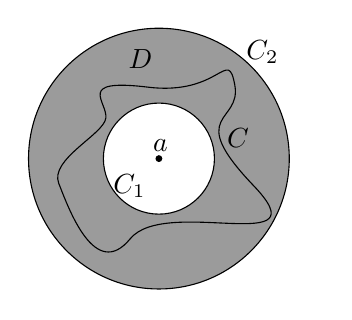
\begin{tikzpicture}[x=0.4,y=0.4,yscale=-1,xscale=1]
%uncomment if require:
\path (0,240.79999542236328);
%set diagram left start at 0, and has height of 240.79999542236328

%Shape: Circle [id:dp6258198346024846] 
\draw  [fill={rgb, 255:red, 155; green, 155; blue, 155 }  ,fill opacity=1 ] (0.77,120.35) .. controls (0.77,55.3) and (53.5,2.57) .. (118.55,2.57) .. controls (183.6,2.57) and (236.32,55.3) .. (236.32,120.35) .. controls (236.32,185.4) and (183.6,238.12) .. (118.55,238.12) .. controls (53.5,238.12) and (0.77,185.4) .. (0.77,120.35) -- cycle ;
%Shape: Circle [id:dp07560041299187703] 
\draw  [fill={rgb, 255:red, 255; green, 255; blue, 255 }  ,fill opacity=1 ] (68.39,120.35) .. controls (68.39,92.65) and (90.85,70.19) .. (118.55,70.19) .. controls (146.25,70.19) and (168.71,92.65) .. (168.71,120.35) .. controls (168.71,148.05) and (146.25,170.51) .. (118.55,170.51) .. controls (90.85,170.51) and (68.39,148.05) .. (68.39,120.35) -- cycle ;
%Shape: Circle [id:dp4185264747557642] 
\draw  [fill={rgb, 255:red, 0; green, 0; blue, 0 }  ,fill opacity=1 ] (116,120.35) .. controls (116,118.94) and (117.14,117.8) .. (118.55,117.8) .. controls (119.96,117.8) and (121.1,118.94) .. (121.1,120.35) .. controls (121.1,121.76) and (119.96,122.9) .. (118.55,122.9) .. controls (117.14,122.9) and (116,121.76) .. (116,120.35) -- cycle ;
%Shape: Polygon Curved [id:ds19792072871438626] 
\draw   (108.6,55.8) .. controls (174.6,63.8) and (180.6,18.8) .. (187.1,53.8) .. controls (193.6,88.8) and (141,78.8) .. (204.1,144.8) .. controls (267.2,210.8) and (124.6,153.8) .. (92.6,192.8) .. controls (60.6,231.8) and (36.72,164.55) .. (28.1,142.8) .. controls (19.47,121.05) and (68.77,98.46) .. (70.6,83.8) .. controls (72.43,69.14) and (42.6,47.8) .. (108.6,55.8) -- cycle ;

% Text Node
\draw (120,108.8) node    {$a$};
% Text Node
\draw (102,30.8) node    {$D$};
% Text Node
\draw (92,144.8) node    {$C_{1}$};
% Text Node
\draw (212,23.8) node    {$C_{2}$};
% Text Node
\draw (190,101.8) node    {$C$};

\end{tikzpicture}

  \caption{単純閉曲線$C$}
\end{wrapfigure}
複素関数$f(z)$が点$a$を孤立特異点に持つとする。
また、点$a$を中心とする円$C_1, C_2$
($C_1$の中に$a$以外の特異点があっても良く、
$C_2$は$C_1$の外側にあるとする)
によって囲まれる領域を$D$とする。
$C_1, C_2$上、領域$D$のいずれにも特異点がないとき、
領域$D$内の任意の$z$に対し、
$D$内にあって$C_1$を囲むような単純閉曲線$C$を使って
\begin{subequations}
\begin{align}
    f(z)
    &= \sum_{n=-\infty}^{\infty}
        c_n (z-a)^n
\label{Laurent series expansion}
\\
    c_n
    &:= \dfrac{1}{2 \pi i}
    \oint_C dz_0 \dfrac{f(z_0)}{(z_0 - a)^{n+1}}
\end{align}
\end{subequations}
が成り立つ。
これを$f(z)$の$a$周りでのLaurent級数展開という。
特に(\ref{Laurent series expansion})の右辺のうち
$c_{-n}\ (n > 0)$が現れる項を特異部(singular part、主要部、principal part)、
$c_{n}\ (n \ge 0)$が現れる項を正則部(regular part、analytic part)という。

\subsubsection{極(pole)、真性特異点(essential singularity)、零点(zero)}

極とは、以下に定める孤立特異点の一種である。
$f(z)$が$a$を$m\ (>0)$位の極($m$-th order pole)
に持つとは、
$f(z)$のLaurent級数展開が$c_{-m} \neq 0$かつ
$n>m$に対し$c_{-n}=0$を満たすことを言う。
特に$1$位の極を単純極(simple pole)、
$2$位の極を二重極(double pole)、
$3$位ならtriple pole、などともいう。

Laurent展開の特異部が有限次で切れず
負べきの項が無限個現れる場合、
$a$を真性特異点(essential singularity)という。

$f(z)$が$a$を$m$位の零点($m$-th order zero)
に持つとは、
$f(z)$のTaylor級数展開
(\ref{Taylor series expansion})
が$c_{m} \neq 0$かつ
$0 \le n < m$に対し$c_{n}=0$を満たすことを言う。
正則関数の零点は孤立し、
この事実を零点孤立の原理という。

\subsubsection{留数定理(Residue theorem)}

Laurent級数展開
\begin{align}
    f(z)
    &= \sum_{n=-\infty}^{\infty}
        c_n (z-a)^n
\end{align}
において、
$\Res{f(z)dz, a} := c_{-1}$を
$f(z)$の点$z=a$における留数(Residue)という。
ただし本来これはRiemann球面$\mathbb{C}P^1$上の
微分形式に対し定義されるものだと示すため、
単に$f(z)$ではなく$f(z)dz$と書いた。
特に、
$f(z)$が$a$を$m$位の極
に持つときは
\begin{align}
    \Res{f(z)dz, a}
    =
    \lim_{z \to a}
    \dfrac{1}{(m-1)!}
    \dfrac{d^{m-1}}{dz^{m-1}}
    \bigg[
        (z-a)^m f(z)
    \bigg]
\end{align}
が成り立つ。
$f(z)$が単純閉曲線$C$内で
$n$個の孤立特異点$a_1,\dots,a_n$を除き正則であるとき
\begin{align}
    \oint_C dz\ f(z)
    =
    2 \pi i \sum_{k=1}^n
    \Res{f(z)dz, a_k}
\end{align}
が成り立つ。

座標変換$u := \dfrac{1}{z}$のもとで
$    g(u)
:=
    f
    \left( \dfrac{1}{u} \right)
$と定義すると、
微分形域は
\begin{align}
    f(z) dz
    =
    f
    \left( \dfrac{1}{u} \right)
    \dfrac{\partial z}{\partial u}
    du
    =
    - \dfrac{ g (u) }{u^2}
    du
\end{align}
のように変換するため、
無限遠点$z = \infty$での留数および
その周りのLaurent展開は
$C_{0}, C_{\infty}$
を原点、無限遠点を囲む
反時計回りの円とし
\begin{subequations}
\begin{align}
    g(u)
&=
    f
    \left( \dfrac{1}{u} \right)
=
    \sum_{n=-\infty}^{\infty}
        c_{n} u^{-n}
=
    \sum_{n=-\infty}^{\infty}
        a_n u^n
\\
    a_n
    &:= \dfrac{1}{2 \pi i}
    \oint_{C_0} du_0 \dfrac{g(u_0)}{u_0^{n+1}}
=
    \dfrac{1}{2 \pi i}
    \oint_{- C_\infty}
        dz_0
        \dfrac{- 1}{z_0^2}
        \dfrac{
            f ( z_0 )
        }{z_0^{-n-1}}
\notag\\&
=
    \dfrac{1}{2 \pi i}
    \oint_{C_\infty}
        dz_0
        \dfrac{
            f ( z_0 )
        }{z_0^{-n+1}}
    = c_{-n}
\\
    \Res{f(z)dz, \infty}
& = c_{-1} =
    \dfrac{1}{2 \pi i}
    \oint_{C_{\infty}} dz\ f(z)
=
    \dfrac{1}{2 \pi i}
    \oint_{- C_{0}} du
    \dfrac{ -1 }{u^2}
    g(u)
=   a_1
\end{align}
\end{subequations}
と書ける。
因子$\dfrac{-1}{u^2}$まで含める事で、
$f(z)$のLaurent展開と$g(z)$のそれが
矛盾なく座標変換で結び付くことが分かる。

\subsubsection{Morera's theorem(モレラの定理)}

以下の意味で、Cauchyの積分定理の逆が成り立つ:
単連結領域$D$で$f(z)$が連続で、
\begin{align}
    \oint_C dz\ f(z) = 0
\end{align}
が$D$内の任意の閉曲線$C$に対し成り立つとする。
このとき$f(z)$は$D$上で正則である。

\newpage
\subsection{初等関数および特殊関数}

\subsubsection{指数関数}

指数関数(exponential function)を
\begin{align}
    \exp(x)
    :=
    \sum_{n=0}^\infty
    \dfrac{x^n}{n!}
\end{align}
により定める。
この級数は複素平面全体で絶対収束
(absolutely convergent)
$\displaystyle
\sum_{n=0}^\infty
\dfrac{|x|^n}{n!}
< \infty
$するため、
$\exp(z)$は整関数
(entire function、複素平面全体で正則な関数)を与える。

\subsubsection{三角関数、双曲線関数}

余弦(cosine)関数、
正弦(sine)関数、
正接(tangent)関数を
指数関数を用いて
\begin{subequations}
\begin{align}
    \cos\theta &:= \dfrac{e^{i\theta} + e^{-i\theta}}{2}
\\
    \sin\theta &:= \dfrac{e^{i\theta} - e^{-i\theta}}{2i}
\\
    \tan\theta &:= \dfrac{\sin\theta}{\cos\theta}
\end{align}
\end{subequations}
と定義する。
これらを総称して三角関数
(trigonometric function、circular function)
という。

同様に双曲線関数(hyperbolic function)を
\begin{subequations}
\begin{align}
    \cosh\theta
    &:=
    \dfrac{e^{\theta} + e^{-\theta}}{2}
    =
    \cos(-i\theta)
\\
    \sinh\theta
    &:=
    \dfrac{e^{\theta} - e^{-\theta}}{2}
    =
    i\sin(-i\theta)
\\
    \tanh\theta
    &:=
    \dfrac{\sinh\theta}{\cosh\theta}
\end{align}
\end{subequations}
と定義する。
それぞれ
hyperbolic cosine、
hyperbolic sine、
hyperbolic tangentと言うが、
$\cosh, \sinh, \tanh$の記号は
cosine hyperbolic(またはコッシュ)、
sine hyperbolic(またはシンチ)、
tangent hyperbolic(またはタンチ)
などと発音される。
native English speakerでも
シンチとかタンチとか言う人は居るが、
分かりづらいだけでなく
はっきり言ってクソダサいので
cosine hyperbolic、sine hyperbolic
などという方が良いと思う。

\subsubsection{無限乗積展開}

三角関数、双曲線関数について
\begin{subequations}
\begin{align}
    \sin \pi x
    &=
    \pi x
    \prod_{n=1}^\infty
    \left(
        1 - \dfrac{x^2}{n^2}
    \right)
\label{infinite product of sine}
\\
    \sinh \pi x
    &=
    \pi x
    \prod_{n=1}^\infty
    \left(
        1 + \dfrac{x^2}{n^2}
    \right)
\label{infinite product of sine hyperbolic}
\\
    \cos \dfrac{\pi x}{2}
    &=
    \prod_{n=1}^\infty
    \left(
        1 - \dfrac{x^2}{(2n-1)^2}
    \right)
\\
    \cosh \dfrac{\pi x}{2}
    &=
    \prod_{n=1}^\infty
    \left(
        1 + \dfrac{x^2}{(2n-1)^2}
    \right)
\end{align}
\end{subequations}
が成り立つ。

\subsubsection{$\Gamma$関数}

$\Gamma$関数は$\Re z > 0$の複素数$z$に対し
\begin{align}
    \Gamma(z)
    := \int_0^\infty dt\ t^{z-1} e^{-t}
\end{align}
により定義され、
その性質
$\Gamma(1) = 1, \Gamma(z+1) = z\Gamma(z)$
から階乗(factorial)
\begin{align}
    \Gamma(n+1) &= n!
    \quad
    (n \in \mathbb{N}_{\ge0})
\end{align}
の複素数への一般化を与える。

重要な応用として、
Gaussian integral(ガウス積分)
\begin{align}
    I :=
    \Gamma\left(\dfrac{1}{2}\right)
    =
    \int_{0}^{\infty} dt\ t^{-1/2}e^{-t}
    =
    2
    \int_{0}^{\infty} dx\ e^{-x^2}
    =
    \int_{-\infty}^{\infty} dx\ e^{-x^2}
    > 0
    \quad(t=x^2)
\end{align}
を求める事を考えよう。
極座標に書き換えると
\begin{align}
    I^2 &=
    \int_{-\infty}^{\infty} dx
    \int_{-\infty}^{\infty} dy
    \ 
        e^{-(x^2 + y^2)}
=
    \int_0^{\infty} dr
    \int_0^{2\pi} r d\theta
    \ 
        e^{-r^2}
\notag\\&=
    2 \pi
    \int_0^{\infty} dr
    \ r 
        e^{-r^2}
=
    \pi
    \int_0^{\infty} dt\ e^{-t}
    \quad(t:=r^2,\ dt = 2 r dr)
\notag\\&=
    \pi\Gamma(1)
    = \pi
\end{align}
すなわち
$\Gamma\left(\dfrac{1}{2}\right)
= I = \sqrt{\pi}$
が求まる。
初等的な置換積分により
\begin{align}
    \int_{-\infty}^{\infty} dx\ e^{-ax^2}
    =
    \sqrt{
        \dfrac{\pi}{a}
    }
\label{gaussian integral}
\end{align}
もすぐ分かり、より一般に
$n \in \mathbb{N}_{\ge0}$に対して
\begin{align}
    \Gamma\left( n + \dfrac{1}{2} \right)
    &=
    \int_0^\infty dt\ t^{n-1/2} e^{-t}
\notag\\&=
    \left[
        \left(
            -
            \dfrac{d}{da}
        \right)^n
        \int_0^\infty dt\ t^{-1/2} e^{-at}
    \right]_{a=1}
\notag\\&=
    \left[
    \left(
        -
        \dfrac{d}{da}
    \right)^n
        a^{-1/2}
        \int_0^\infty a dt\ (at)^{-1/2} e^{-at}
    \right]_{a=1}
\notag\\&=
    \left[
    \left(
        -
        \dfrac{d}{da}
    \right)^n
    \sqrt{
        \dfrac{\pi}{a}
    }
    \right]_{a=1}
\notag\\&=
    \dfrac{(2n-1)!!}{2^{n}}\sqrt{\pi}
\label{Gamma function at half integer}
\end{align}
が得られる。
ただしdouble factorial(二重階乗)を
偶数、奇数それぞれについて
\begin{subequations}
\begin{align}
    (2n)!!
    &:=
    \prod_{i=1}^n (2i)
    =2\cdot4\cdot6\cdots(2n-2)(2n)
\\
    (2n-1)!!
    &:=
    \prod_{i=1}^n (2i-1)
    =
    1\cdot3\cdot5\cdots(2n-3)(2n-1)
\end{align}
\end{subequations}
と定義した。

$\Gamma$関数の$\Re z < 0$への解析接続は
Euler's reflection formula
\begin{align}
    \Gamma(z) \Gamma(1-z)
    =
    \dfrac{\pi}{\sin(\pi z)}
\label{Euler's reflection formula}
\end{align}
で与えられ、
この公式からも
$\Gamma \left(\dfrac{1}{2}\right) = \sqrt{\pi}$
が確かめられる。
$\Gamma$関数は零点を持たないが
(\ref{Euler's reflection formula})からも分かるように
$n \in \mathbb{N}_{\ge0}$に対して
$x = - n$を$1$位の極に持ち、
その周りで
\begin{align}
    \Gamma(x)
    &=
    \dfrac{(-1)^n}{n!}
    \left(
        \dfrac{1}{x+n} - \gamma
        + \sum_{k=1}^n \dfrac{1}{k}
    \right)
    + \mathcal{O}(x+n)
\\
    \gamma
    &:=
    \lim_{n\to\infty}
    \left(
        \sum_{k=1}^n \dfrac{1}{k} 
        -
        \log n
    \right)
    \simeq 0.5772
\end{align}
と展開できる。
ただし$\gamma$は
Euler-Mascheroni constant(オイラー定数)である。

なお、上で与えた$\Gamma$関数の解析接続や
極周りでの展開は
Euler-Mascheroni constantを使って
\begin{subequations}
\begin{align}
    \dfrac{
        e^{- \gamma x}
    }{
        \Gamma(x+1)
    }
    &=
    \prod_{n=1}^\infty
    \left(
        1 + \dfrac{x}{n}
    \right)
    e^{- x / n}
\\
    \dfrac{\sin \pi x}{\pi x}
    &=
    \prod_{n = - \infty}^\infty
    \left(
        1 + \dfrac{x}{n}
    \right)
    e^{- x / n}
\end{align}
\end{subequations}
なる無限乗積展開から正当化される。

\subsubsection{Fresnel integral}

Fresnel integral(フレネル積分)は
Gauss積分
(\ref{gaussian integral})の
$\alpha \in \mathbb{C}$への拡張であり、
\begin{align}
    \int_{-\infty}^{\infty}
    dx\ e^{- \alpha x^2}
    =
    \sqrt{
        \dfrac{\pi}{\alpha}
    }
    \quad
    \text{ for $\Re \alpha \ge 0$}
\label{fresnel integral}
\end{align}
と求まる。

\subsubsection{
    超幾何関数
    (confluent hyper-geometric function)
}

Pochhammer symbolを
\begin{align}
    (x)_n
    &:=
    \dfrac{\Gamma(x+n)}{\Gamma(x)}
\end{align}
で定義する。
一般化された超幾何関数
(generalized hyper-geometric function)は
$|z| < 1$で収束するべき級数
\begin{align}
    {}_r F_s
    (
        a_1, \dots, a_r;
        b_1, \dots, a_s;
        z
    )
    &:=
    \sum_{n=0}^{\infty}
    \dfrac{ (a_1)_n \cdots (a_r)_n }{
      (b_1)_n \cdots (b_s)_n
    }
    \dfrac{z^n}{n!}  
\end{align}
で定義される解析関数で、
$a_1, \dots, a_r$同士、
または$b_1, \dots, b_s$同士を交換しても
全く同じ関数を与える。

このうち、特に
\begin{align}
    F(a, b, c; z)
    :=
    {}_2 F_1 (a, b; c; z)
\end{align}
をGaussの超幾何関数、
\begin{align}
    F(a, b; z)
    :=
    {}_1 F_1(a; b; z)
\end{align}
を合流型超幾何関数
(confluent hyper-geometric function)、
あるいは
Kummerの関数などという。

\subsubsection{Sturm-Liouville equation}

任意の$2$階線形微分方程式は
Sturm-Liouville equation
(スツルム・リウビル型微分方程式)
に変形できる。
その解についてはかなり一般論
(離散固有値を持つ、
直交性を満たす、
多くの場合Rodrigues' formula
(ロドリゲス表示、ロドリグ公式など)で書けるなど)
が存在し、
Sturm-Liouville理論と呼ばれる。

\subsubsection{Hermite多項式}
\label{hermite polynomial}

Hermite多項式はHermite微分方程式
\begin{align}
    y'' + x y' + n y = 0
\end{align}
の解であり、
$H_0(x) = 1, H_1(x) = x$として次の漸化式
\begin{subequations}
\begin{align}
    0
    &=
    H_{n+1}(x)
    -
    x H_n(x)
    +
    n H_{n-1}(x)
\\
    H_n'(x)
    &=
    n H_{n-1}(x)
\end{align}
\label{hermite polynomial recurrence relation}
\end{subequations}
および直交性
\begin{align}
    \int dx H_n(x) H_m(x) e^{-x^2/2}
    =
    n! \sqrt{2 \pi}
    \delta_{nm}
\label{normality of hermite polynomial}
\end{align}
を満たす。

Rodrigues' formulaは
\begin{align}
    H_n(x)
    =
    (-1)^n e^{ + x^2 / 2 }
    \dfrac{d^n}{dx^n}
    e^{ - x^2 / 2 }
\label{hermite rodrigues formula}
\end{align}
と与えられ、
合流型超幾何関数$F$を使って
\begin{subequations}
\begin{align}
    H_{2n}(x)
    :=
        (-1)^n
        (2 n - 1)!!
    F(-n, 1/2; x^2/2)
\\
    H_{2n+1}(x)
    :=
        (-1)^n
        (2 n + 1)!!
    F(-n, 3/2; x^2/2)
\end{align}
\end{subequations}
とも書かれる。

\subsubsection{Bessel関数}

第一種Bessel関数
(Bessel function of the first kind)
は一般化された超幾何関数を用い
\begin{subequations}
\begin{align}
    J_\nu (z)
&=
    \dfrac{ (z/2)^\nu }
        { \Gamma(\nu + 1) }
    {}_0 F_1 \left(
        \nu + 1; - \dfrac{z^2}{4}
    \right)
\\&=
    \dfrac{ (z/2)^\nu }
        { \Gamma(\nu + 1) }
    e^{- i z}
    {}_1 F_1 \left(
        \nu + \dfrac{1}{2};
        2 \nu + 1;
        2 i z
    \right)
\end{align}
\end{subequations}
の表示を持つ。
平面波はBessel関数により
\begin{align}
    e^{ i z \sin \theta }
&=
    \sum_{n = - \infty}^{\infty}
        J_n(z)
        e^{i n \theta}
\label{plane wave expanded by bessel 1st}
\end{align}
と展開される。

$\Re \nu > -\dfrac{1}{2},
\Re z > 0$
の領域では
Lommelの積分表示
\begin{align}
    \dfrac{
        \pi^{1/2}
        \Gamma(\nu + \frac{1}{2})
    }
    {(z/2)^\nu}
    J_{\nu}(z)
&=
    \int_{0}^\pi
        d \theta
        \cos (z \cos \theta)
        \sin^{2 \nu} \theta
\label{lommel integral formula for Bessel 1st}
\end{align}
によっても表示できる。

\newpage
\subsection{Fourier級数展開、Fourier変換}

\subsubsection{Fourier級数展開}

周期$2L$の周期関数$f(x)$、
あるいは区間$(a, a + 2L)$を定義域とする関数$f(x)$を
周期関数に拡張したものについて
\begin{subequations}
\begin{align}
    \tilde{f}(x)
    &:=
    \sum_{n=-\infty}^\infty
    c_n e^{ i\frac{n \pi}{L}x }
\\
    c_n
    &:=
    \dfrac{1}{2L} \int_{-L}^L dx\ 
    f(x) e^{ - i\frac{n \pi}{L}x }
\end{align}
\end{subequations}
を複素Fourier series(フーリエ級数)、
\begin{subequations}
\begin{align}
    \tilde{f}(x)
    &:=
    \dfrac{a_0}{2}
    +
    \sum_{n=1}^\infty
    \left(
        a_n \cos \dfrac{n \pi}{L}x
        +
        b_n \sin \dfrac{n \pi}{L}x
    \right)
\\
    a_n
    &:=
    \dfrac{1}{L} \int_{-L}^L dx\ 
    f(x) \cos\dfrac{n \pi}{L}x
\\
    b_n
    &:=
    \dfrac{1}{L} \int_{-L}^L dx\ 
    f(x) \sin\dfrac{n \pi}{L}x
\end{align}
\end{subequations}
をFourier seriesなどという。
特に$\forall n$に対して
$a_n = 0$のときFourier正弦展開、
$b_n = 0$のときFourier余弦展開
などということもある。

$f(x)$が区分的になめらか、
つまり$f(x), f'(x)$がともに区分的に連続ならば
そのFourier級数は各点収束し、収束先は
\begin{align}
    \tilde{f}(x) = \dfrac{f(x+0) + f(x-0)}{2}
\end{align}
で与えられる。
$f(x)$が連続ならさらに強くFourier級数は関数列として一様収束するが、
不連続関数のFourier級数は一様収束せず、
広義一様収束、ないしコンパクト一様収束
(uniformly convergent on compact sets)
しかしない。
不連続点$x = a$ s.t.
$\mathrm{Disc}(f,a) := f(a+0) - f(a-0) \neq 0$の付近では
振幅$\mathrm{Disc}(f,a) \times 0.08949\dots$程度の振動が起こり、
ギブス現象(Gibbs phenomenon)とか呼ばれる。
激しく振動する成分はRiemann-Lebesgue lemmaより積分に寄与しないので、
$L^2$-normで見る限り(\ref{convergence of norm})と全く同様に
\begin{subequations}
\begin{align}
    \lim_{N\to\infty}\bigg|\bigg|
        f(x) - \tilde{f}_N(x)
    \bigg|\bigg|^2
    &=
    \lim_{N\to\infty}\int dx
    \Big| f(x) - \tilde{f}_N(x) \Big|^2
    = 0
\\
    \tilde{f}_N(x)
    &:=
    \sum_{n=-N}^N
    c_n e^{ i\frac{n \pi}{L}x }
\end{align}
\end{subequations}
のように収束している、ということである。

\subsubsection{Fourier変換}

周期関数でないより一般の関数もFourier級数と同様に
三角関数で展開したいというのは自然な要求だろう。
特にこれは微分方程式を解くために役立つ。
急減少関数$f(x)$のFourier transform(フーリエ変換)$\tilde{f}(k)$
および
inverse Fourier transform(逆フーリエ変換)を
\begin{subequations}
\begin{align}
    \tilde{f}(k)
    &:=
    \int dx\ f(x) e^{-ikx}
\\
    f(x)
    &=
    \dfrac{1}{2\pi}\int dk\ 
    \tilde{f}(k) e^{+ikx}
\end{align}
\label{fourier transf}
\end{subequations}
で定める。
特に、逆変換はDirac delta関数のFourier表示
(\ref{dirac delta fourier representation})
により正当化される。
$\dfrac{1}{2\pi}$を
Fourier変換(逆変換でなく)の定義に付けて
$\displaystyle
\tilde{f}(k) = \dfrac{1}{2\pi}
\int dx\ f(x) e^{-ikx}$
としたり、
$k$の符号を逆にして
$\displaystyle
\tilde{f}(k) =
\int dx\ f(x) e^{+ikx}$としたり、
(\ref{plain wave in qm})のように
波動関数の規格化を気にする量子力学では
$\displaystyle
    \braket{ x | f }
    =
    \dfrac{1}{\sqrt{2\pi}}
    \int dk\ \braket{k | f} e^{+ikx}
    ,
    \braket{ k | f }
    =
    \dfrac{1}{\sqrt{2\pi}}
    \int dx\ \braket{x | f} e^{-ikx}
$
のように$\dfrac{1}{\sqrt{2\pi}}$が
変換と逆変換の両方に現れたり、
数値計算や結晶学では角周波数でなく周波数を用いて
$\displaystyle
\tilde{f}(k) =
\int dx\ f(x) e^{+2\pi ikx}$としたり、
とにかく無数の流儀があるが、本質積な違いは何もない。

Fourier変換は不確定性関係という良くない性質を持つため、
画像処理などの分野ではwavelet解析という拡張を考えることがある。

\newpage
\subsection{微分幾何学}

\subsubsection{計量}

計量(metric tensor)
$g_{ij} = g_{ji}$は対称tensorで、
その逆行列を$g^{ij} := (g^{-1})^{ij}$
(すなわち
$g_{ik} g^{kj} = \delta_i^j$)、
行列式を$g = \det (g_{ij})$と書く。
計量の成分を示すときは行列で書くか、
$ds^2 = g_{ij} dx^i dx^j$の全ての項を
書き下す。
特に、後者の記法では
非対角項($i \neq j$)に対して
対称性から必ず
計量の成分$g_{ij}$の$2$倍
が現れる事に注意しよう。
例えば二次元直交座標を用いて
$z = x + i y,
\overline{z} = x - i y$
と定義される座標での計量は
\begin{subequations}
\begin{align}
    (g_{ij})
&=
    \begin{pmatrix}
        0 & \dfrac{1}{2}
    \\
        \dfrac{1}{2} & 0
    \end{pmatrix}
\notag\\
    (g^{ij})
&=
    \begin{pmatrix}
        0 & 2
    \\
        2 & 0
    \end{pmatrix}
\\
    g
&=
    \det(g_{ij})
    = - \dfrac{1}{4}
\\
    ds^2
&=
    dx^2 + dy^2
=
    d z
    d \overline{z}
=
    g_{z \overline{z}}
    d z
    d \overline{z}
+
    g_{\overline{z} z}
    d \overline{z}
    d z
\neq \dfrac{1}{2} 
    d z
    d \overline{z}
\end{align}
\end{subequations}
となる。

座標$x^i$における
計量$g_{ij}$が与えられているとき、
$\partial_i = \dfrac{\partial}{\partial x^i}$として
scalar関数$f(x)$に作用するLaplacianは
\begin{align}
    \Delta f(x)
    =
    \dfrac{1}{ \sqrt {g} }
    \partial_i
    \left(
        g^{ij}
        \sqrt{ g }
        \partial_j
        f (x)
    \right)
\label{laplacian of scalar in terms of metric}
\end{align}
と書くことが出来る。
ただし
vectorやtensorに作用するLaplacianは
このように書くことが出来ないので注意せよ。

\subsubsection{$n$次元極座標}

$1$次元極座標は
(連続な角度変数が取れないため特殊で)
$(r, \mathrm{sgn}(x)) = (|x|, \pm 1)$
で、
$2$次元極座標は
$(x, y) = (r \cos \theta, r \sin \theta)$
で、
$3$次元球座標は
$(x, y, z)
=
    (r \sin \theta \sin \phi,
    r \sin \theta \cos \phi,
    r \cos \theta)$
で与えられる。

一般の$n (\ge 3)$次元の極座標
(polar coordinates、
球座標、spherical coordinates)
$(r, \theta_1, \theta_2,
\dots, \theta_{n-1})$
は直交座標
$(x_1, \dots, x_n)$を用いて
\begin{subequations}
\begin{align}
    r :=& \sqrt{
        \sum_{i=1}^n
        (x_i)^2
    }
&
    (0 \le\ &r < \infty)
\\
    x_n
    =:&\ 
    r \cos \theta_1
&
    (0 \le\ &\theta_1 \le \pi)
\\
    x_{n-1}
    =:&\ 
    r \cos \theta_2
    \sin \theta_1
&
    (0 \le\ &\theta_2 \le \pi)
\\\notag
    &
    \vdots
    &
    \vdots
\\
    x_{n-i}
    =:&\ 
    r
    \cos \theta_{i+1}
    \prod_{j=1}^{i}
    \sin \theta_j
&
    (0 \le\ &\theta_{i+1} \le \pi)
\\\notag
    &
    \vdots
    &
    \vdots
\\
    x_{2}
    =:&\ 
    r
    \cos \theta_{n-1}
    \prod_{j=1}^{n-2}
    \sin \theta_j
&
    (0 \le\ &\theta_{n-1} < 2 \pi)
\\
    x_{1}
    =:&\ 
    r
    \prod_{j=1}^{n-1}
    \sin \theta_j
\end{align}
\label{n dimensional spherical coordinates}
\end{subequations}
と定義される。
ただし、
$1 \le i \le n-2$に対して
$x_{n-i+1}$の表式に
$\cos \theta_i$が$1$回だけ現れるため、
この因子が左辺の符号を決める
(つまり$\sin \theta_i$が正の値しか取れない)よう
$\theta_i$の取り得る範囲を選んだ。
こうしておけば
$(x_1, \dots, x_n)$と
$(r, \theta_1, \dots, \theta_{n-1})$
が一対一で対応するためである。
$i = n - 1$の時だけが特殊で、
$x_1, x_2$が任意の実数を動くためには
$\cos \theta_{n-1}$だけでなく
$\sin \theta_{n-1}$も正負の値を動けなければならない事に注意せよ。
特に、
$\dfrac
    { x_{1} }
    { x_{2} }
=
    \tan \theta_{n-1}
$
及び
$
\dfrac
    { x_{n - i} }
    { x_{n - (i - 1)} }
=
    \tan \theta_{i}
    \cos \theta_{i+1}
$
$(1 \le i \le n - 2)$
が成り立つ。

明らかに
\begin{subequations}
\begin{align}
    \dfrac{\partial x_i}
        {\partial r}
&=
    \begin{cases}
    \displaystyle
        \prod_{j=1}^{n - 1}
        \sin \theta_j
    &(i = 1)
    \\
    \displaystyle
        \cos \theta_{n - i + 1}
        \prod_{j=1}^{n - i}
        \sin \theta_j
    &(2 \le i \le n - 1)
    \\
    \displaystyle
        \cos \theta_{1}
    &(i = n)
    \end{cases}
\\
    \dfrac{\partial x_i}
        {\partial \theta_j}
&=
    \begin{cases}
    \displaystyle
        r \cos \theta_j
        \prod_{k=1 (\neq j)}^{n-1}
        \sin \theta_k
    &(i = 1 \le j \le n - 1)
    \\
    \displaystyle
        r \cos \theta_{n - i + 1}
        \cos \theta_j
        \prod_{k=1 (\neq j)}^{n - i}
        \sin \theta_k
    &(2 \le i \le n - j \le n - 1)
    \\
    \displaystyle
        -
        r \sin \theta_{n - i + 1}
        \prod_{k=1}^{n - i}
        \sin \theta_k
    &(2 \le i = n - j + 1 \le n - 1)
    \\
    \displaystyle
        0
    &(2 \le n-j+1 \le i - 1 < i \le n - 1)
    \\
    \displaystyle
        -
        r \sin \theta_1
    &(1 = j < i = n)
    \\
    \displaystyle
        0
    &(1 < j < i = n)
    \end{cases}
\end{align}
\end{subequations}
が分かる。
この座標での計量は
\begin{align}
    &
    ds^2
=
    g_{ij} dx^i dx^j
:=
    \delta_{ab}
    \dfrac{\partial x^a}{\partial \phi^i}
    \dfrac{\partial x^b}{\partial \phi^j}
    d \phi^i d\phi^j
\notag\\&
=
    d r^2
\underset{
\displaystyle
\color{blue}
    =
    \Bigg(
    \underset{
    \displaystyle
    = \sin^2 \theta_1
    }{\underline{
        \prod_{j=1}^{n - 1}
        \sin^2 \theta_j
    +
    \sum_{i = 2}^{n-1}
        \cos^2 \theta_{i}
        \prod_{j=1}^{i - 1}
        \sin^2 \theta_j
    }}
    +
        \cos^2 \theta_{1}
    \Bigg)
    = 1
}{\underline{
    \left(
        \prod_{j=1}^{n - 1}
        \sin^2 \theta_j
    +
    \sum_{i = 2}^{n-1}
        \cos^2 \theta_{n - i + 1}
        \prod_{j=1}^{n - i}
        \sin^2 \theta_j
    +
        \cos^2 \theta_{1}
    \right)
}}
\notag\\&\qquad
    +
    (dr d\theta_1 + d\theta_1 dr)
\underset{
\displaystyle
\color{blue}
    =
    r \sin \theta_1
    \cos \theta_1
    \Bigg(
    \underset{
    \displaystyle
        \text{$dr^2$の項と同様に計算すると$1$}
    }{\underline{
        \prod_{q=2}^{n-1}
        \sin^2 \theta_q
    +
    \sum_{i = 2}^{n - 1}
        \cos^2 \theta_{i}
        r \cos \theta_1
        \prod_{q=2}^{i-1}
        \sin^2 \theta_q
    }}
    -
        1
    \Bigg)
    = 0
}{\underline{
    \Bigg(
        \prod_{p=1}^{n - 1}
        \sin \theta_p
        r \cos \theta_1
        \prod_{q=2}^{n-1}
        \sin \theta_q
    +
    \sum_{i = 2}^{n - 1}
        \cos^2 \theta_{n - i + 1}
        \prod_{p=1}^{n - i}
        \sin \theta_p
        r \cos \theta_1
        \prod_{q=2}^{n - i}
        \sin \theta_q
    -
        \cos \theta_1
        r \sin \theta_1
    \Bigg)
}}
\notag\\&\qquad
    +
    \sum_{k=2}^{n-1}
    (dr d\theta_k + d\theta_k dr)
    \Bigg(
\underline{
        \prod_{p=1}^{n - 1}
        \sin \theta_p
        r \cos \theta_k
        \prod_{q=1 (\neq k)}^{n-1}
        \sin \theta_q
    +
    \sum_{i = 2}^{n-k}
        \cos^2 \theta_{n - i + 1}
        \prod_{p=1}^{n - i}
        \sin \theta_p
        r
        \cos \theta_k
        \prod_{q=1 (\neq k)}^{n - i(\ge k)}
        \sin \theta_q
}
\notag\\&\qquad\qquad
\underset{
\displaystyle
\color{blue}
    =
    r \tan^{-1} \theta_k
    \bigg(
    \underbrace{
        \prod_{p=1}^{n - 1}
        \sin^2 \theta_p
    +
    \sum_{i = k+1}^{n - 1}
        \cos^2 \theta_{i}
        \prod_{p=1}^{i - 1}
        \sin^2 \theta_p
    }_{\substack{
    \displaystyle
    = \sin^2 \theta_1
        -
        \sum_{i = 2}^k
        \cos^2 \theta_{i}
        \prod_{p=1}^{i - 1}
        \sin^2 \theta_p
    \\
    \displaystyle
    =
        \sin^2 \theta_1
        -
        \bigg(
            \sin^2 \theta_1
        -
            \prod_{p=1}^{k}
            \sin^2 \theta_p
        \bigg)
    }}
    -
    \underbrace{
        \sin^2 \theta_k
        \prod_{p=1}^{k - 1}
        \sin^2 \theta_p
    }_{\substack{
    \displaystyle
        =
        \prod_{p=1}^{k}
        \sin^2 \theta_p
    }}
    \bigg)
    = 0
}{\underline{
    -
        \cos \theta_{k}
        \prod_{p=1}^{k - 1}
        \sin \theta_p
        r
        \sin \theta_{k}
        \prod_{q=1}^{k - 1}
        \sin \theta_q
    \Bigg)
}}
\notag\\&\qquad
    + d \theta_1^2
    \bigg\{
\underbrace{
        r^2 \cos^2 \theta_{1}
        \prod_{p=2}^{n-1}
        \sin^2 \theta_p
    +
    \sum_{i = 2}^{n-1}
        r^2 \cos^2 \theta_{n - i + 1}
        \cos^2 \theta_1
        \prod_{p=2}^{n-i}
        \sin^2 \theta_p
}_{\substack{
    \displaystyle
    \color{blue}\text{
    $dr d\theta_1$の項と同様に
    $r^2 \cos^2 \theta_1$
}}}
    +
        r^2 \sin^2 \theta_1
    \bigg\}
\notag\\&\qquad
    +
    \sum_{k = 2}^{n - 2}
    d \theta_k^2
\underbrace{
    \Bigg\{
        r^2 \cos^2 \theta_k
        \prod_{p=1 (\neq k)}^{n-1}
        \sin^2 \theta_p
    +
    \sum_{i = 2}^{n - k}
        r^2 \cos^2 \theta_{n - i + 1}
        \cos^2 \theta_{k}
        \prod_{p=1 (\neq k)}^{n-i(\ge k)}
        \sin^2 \theta_p
}_{\substack{
\displaystyle
\color{blue}
    = r^2 \tan^{-2} \theta_k
    \Bigg(
\underbrace{
        \prod_{p=1}^{n-1}
        \sin^2 \theta_p
    +
    \sum_{i = k+1}^{n - 1}
        \cos^2 \theta_{i}
        \prod_{p=1}^{i-1}
        \sin^2 \theta_p
}_{\substack{
\displaystyle
\color{blue}
    \text{
        $dr d\theta_k$の項と同様に
        $\displaystyle
        \prod_{p=1}^{k}
        \sin^2 \theta_p
        $
    }
}}
    \Bigg)
    = r^2 \cos^2 \theta_k
    \prod_{p=1}^{k-1}
    \sin^2 \theta_p
\\
}}
% \notag\\&\qquad\qquad
    +
\underbrace{
        r^2 \sin^2 \theta_{k}
        \prod_{p=1}^{k-1}
        \sin^2 \theta_p
}_{\substack{
\displaystyle
\color{blue}
    =
    r^2 \bigg(
        \prod_{p=1}^{k}
        \sin^2 \theta_p
    \bigg)
}}
    \Bigg\}
\notag\\&\qquad
    + d \theta_{n-1}^2
    \bigg\{
        r^2 \cos^2 \theta_{n-1}
        \prod_{p=1}^{n-2}
        \sin^2 \theta_p
    +
        r^2 \sin^2 \theta_{n-1}
        \prod_{p=1}^{n-2}
        \sin^2 \theta_p
    \bigg\}
    -
\underbrace{
    \sum_{k = 1}^{n - 1}
    \sum_{l \neq k}
    d \theta_k
    d \theta_l
}_{\substack{
\displaystyle
\color{blue} =
    2
    \sum_{l < k}
    d \theta_k
    d \theta_l
%\\ \displaystyle \color{blue}
=
    2 \sum_{k = 2}^{n - 1}
    \sum_{l = 1}^{k-1}
    d \theta_k
    d \theta_l
}}
    \underbrace{
    \bigg\{
        \cdots
    \bigg\}
    }_{\substack{\displaystyle
        \color{blue} = 0
    }}
\notag\\&
=
    d r^2
+
    r^2
\left(
        d \theta_1^2
    +
    \sum_{k=2}^{n-1}
        d\theta_k^2
    \prod_{p=1}^{k-1}
        \sin^2 \theta_p
\right)
\label{n dim spherical coord metric}
\end{align}
と計算できる
($l \neq k$の項が消えることを確かめてみよ)。
特に、$g_{ij}$が対角なことから
\begin{align}
    g =
    \det ( g_{ij} )
=
    1 \cdot (r^2)^{n-1}
    \prod_{k=2}^{n-1}
    \prod_{p=1}^{k-1}
        \sin^2 \theta_p
=
    r^{2(n-1)}
    \prod_{j = 1}^{n-2}
    \sin^{2(n - j - 1)} \theta_j
\end{align}
がすぐに分かる。

$n (\ge 3)$次元における体積要素は
Jacobian
\begin{align}
    \frac{\partial(x_1, x_2, \cdots, x_n)}
    {\partial(r, \theta_1, \cdots, \theta_{n-1})}
=
    \det
\left(
    \dfrac{\partial x_i}{\partial \phi_j}
\right)
=
    \sqrt{ g }
=
    r^{n-1}
    \prod_{j = 1}^{n-2}
    \sin^{n - j - 1} \theta_j
\label{jacobian for spherical coordinates}
\end{align}
に気を付けて
\begin{align}
    d^n x
&=
    \prod_{i = 1}^n
    d x_i
=
    \frac{\partial(x_1, x_2, \cdots, x_n)}
    {\partial(r, \theta_1, \cdots, \theta_{n-1})}
    \prod_{i = 1}^n
    d \phi_i
=
    d r d \theta_1
        \cdots d \theta_{n-1}
    r^{n-1}
    \prod_{j = 1}^{n-2}
    \sin^{n - j - 1} \theta_j
\\\notag&
\bigg(
=
    (dr)
    (r d \theta_1)
    (r \sin \theta_1 d \theta_2)
\cdots
    (r \prod_{j = 1}^i
    \sin \theta_j d \theta_i)
\cdots
    (r \prod_{j = 1}^n
    \sin \theta_j d \theta_n)
\bigg)
\end{align}
で与えられ、
特に半径$R$の$n$次元球の体積は
\begin{align}
    V_n(R)
&:=
    \int_{r \le R} d^n x
=
    \int_0^R
        dr
    \int_0^{2 \pi}
        d \theta_{n-1}
    \prod_{i=1}^{n-2}
    \left[
        \int_0^{\pi}
            d \theta_i
    \right]
    r^{n-1}
    \prod_{j = 1}^{n-2}
    \sin^{n - j - 1} \theta_j
\notag\\&
=
    \int_0^R
        dr\ 
    r^{n-1}
    \int_0^{2 \pi}
        d \theta_{n-1}
    \prod_{i=1}^{n-2}
    \left[
        \int_0^{\pi}
            d \theta_i
        \sin^{n - i - 1} \theta_i
    \right]
\notag\\&
=
    \dfrac{R^n}{n}
    2 \pi
    \prod_{i=1}^{n-2}
    \left[
        \sqrt{\pi}
        \dfrac{\Gamma(\frac{n - i}{2})}
        {\Gamma(\frac{n - i + 1}{2})}
    \right]
\notag\\&
=
    \dfrac{R^n}{n}
    S_{n-1}
\end{align}
と求まる。
ここで$S_{n-1}$は$n-1$次元
単位球面$S^{n-1}$の面積で、
対応する立体角を$d^{n-1} \Omega$
と書くことにすると
$\Gamma$関数の半整数での値
(\ref{Gamma function at half integer})
を用いて
\begin{align}
    S_{n-1}
&=
    \int_{r = 1}
        d^{n-1} \Omega
=
    2 \pi
    \prod_{i=1}^{n-2}
    \left[
        \sqrt{\pi}
        \dfrac{\Gamma(\frac{n - i}{2})}
        {\Gamma(\frac{n - i + 1}{2})}
    \right]
=
    2 \pi
    \pi^{(n-2)/2}
    \dfrac{
        \cancel{
            \Gamma(\frac{n - 1}{2})
        }
    }
        {\Gamma(\frac{n}{2})}
    \dfrac{
        \cancel{
            \Gamma(\frac{n - 2}{2})
        }
    }
        {\cancel{
            \Gamma(\frac{n - 1}{2})
        }}
    \cdots
    \dfrac{\Gamma(\frac{n - (n-2)}{2})}
        {\cancel{
            \Gamma(\frac{n - (n-2) + 1}{2})
        }}
\notag\\&
=
    2
    \pi^{n/2}
    \dfrac{\Gamma(1)}
        {\Gamma(\frac{n}{2})}
=
    \dfrac{ 2 \pi^{n/2} }
        {\Gamma(\frac{n}{2})}
\label{surface area of n dimensional sphere}
\end{align}
と書ける。

公式(\ref{laplacian of scalar in terms of metric})
に
計量
(\ref{n dim spherical coord metric})
および
Jacobian
(\ref{jacobian for spherical coordinates})
を代入すると、
$n$次元球座標でscalarに作用する
Laplacianは
\begin{align}
    \Delta f(x)
&=
    \dfrac{1}{ \sqrt {g} }
    \partial_i
    \left(
        g^{ij}
        \sqrt{ g }
        \partial_j
        f (x)
    \right)
\notag\\&
=
    \dfrac{1}{
    \displaystyle
        r^{n-1}
        \prod_{p = 1}^{n-2}
        \sin^{n - p - 1} \theta_p
    }
    \partial_i
    \left(
        g^{ij}
        r^{n-1}
        \prod_{q = 1}^{n-2}
        \sin^{n - q - 1} \theta_q
        \partial_j
        f (x)
    \right)
\notag\\&
=
    \dfrac{1}{
    \displaystyle
        r^{n-1}
    }
    \partial_r
    \left(
        r^{n-1}
        \partial_r
        f
    \right)
+
    \dfrac{1}{
    \displaystyle
        \sin^{n - 2} \theta_1
    }
    \partial_1
    \left(
        r^{-2}
        \sin^{n - 2} \theta_1
        \partial_1
        f
    \right)
\notag\\&\qquad
+
\sum_{k = 2}^{n-2}
    \dfrac{1}{
    \displaystyle
        \sin^{n - k - 1} \theta_k
    }
    \partial_k
    \left(
    \left[
        r^{-2}
        \prod_{p=1}^{k-1}
        \sin^{-2} \theta_p
    \right]
        \sin^{n - k - 1} \theta_k
        \partial_k
        f
    \right)
\notag\\&\qquad
+
    \partial_{n-1}
    \left(
        \left[
            r^{-2}
            \prod_{p=1}^{n-2}
            \sin^{-2} \theta_p
        \right]
        \partial_{n-1}
        f
    \right)
\notag\\&
=
    \dfrac{1}{
    \displaystyle
        r^{n-1}
    }
    \partial_r
    \left(
        r^{n-1}
        \partial_r
        f
    \right)
+
    \dfrac{1}{r^2}
        \Delta_{S^{n-1}}
        f
\label{n dim laplacian in polar coordinates}
\end{align}
と書けることが分かる。
第$1$項は
$    \dfrac{1}{
    \displaystyle
        r^{n-1}
    }
    \partial_r
    \left(
        r^{n-1}
        \partial_r
    \right)
=
    \partial_r^2
    +
    \dfrac{n-1}{ r }
        \partial_r
$と書いても同じことである。
ただし、角度方向つまり
球面$S^{n-1}$上のLaplace-Beltrami operator
(ラプラス・ベルトラミ作用素)を
\begin{align}
    \Delta_{S^{n-1}} f
&:=
        \dfrac{1}{
    \displaystyle
        \sin^{n - 2} \theta_1
    }
    \partial_1
    \left(
        \sin^{n - 2} \theta_1
        \partial_1
        f
    \right)
+
\sum_{k = 2}^{n-2}
    \dfrac{1}{
    \displaystyle
        \sin^{n - k - 1} \theta_k
        \prod_{p=1}^{k-1}
        \sin^{2} \theta_p
    }
    \partial_k
    \left(
        \sin^{n - k - 1} \theta_k
        \partial_k
        f
    \right)
\notag\\&\qquad
+
    \dfrac{1}{
    \displaystyle
        \prod_{p=1}^{n-2}
        \sin^{2} \theta_p
    }
    \partial_{n-1}^2
        f
\notag\\&
=
    \sum_{k = 1}^{n - 1}
    \prod_{p = 1}^{k}
    \dfrac{1}{\sin^2 \theta_p}
    \dfrac{1}{\sin^{n - k - 3} \theta_k}
    \partial_k
    \left(
        \sin^{n - k - 1} \theta_k
        \partial_k
        f
    \right)
\label{spherical Laplacian}
\end{align}
と定義した。
この微分作用素は球Laplacian
(spherical Laplacian)と呼ばれる事もあり、
物理の文脈では
角運動量の大きさoperator
(\ref{the square of the magnitude of the orbital angular momentum})
の$\bm{x}$-表示に他ならない。
$\Delta_{S^{n-1}}$の固有関数を
球面調和関数と呼ぶが、
これも$\hat{L}^2$の固有状態
$\ket{j, m}$に対応する波動関数と解釈できる。
なお、この結果は$n = 2,3$で
\begin{align}
    \Delta_{(2)}
    &=
    \dfrac{1}{r}
        \partial_r
        (r \partial_r)
    +
    \dfrac{1}{r^2}
    \Delta_{S^1}
\notag\\&
=
    \dfrac{1}{r}
        r \partial_r^2
    +
    \dfrac{1}{r}
        \partial_r
    +
    \dfrac{1}{r^2}
    \dfrac{1}{\sin^2 \theta}
    \dfrac{1}{\sin^{2-1-3} \theta}
    \partial_\theta
    (\sin^{2-1-1} \theta \partial_\theta)
\notag\\&
=
        \partial_r^2
    +
        \dfrac{1}{r}
        \partial_r
    +
    \dfrac{1}{r^2}
    \partial_\theta^2
\\
    \Delta_{(3)}
    &=
    \dfrac{1}{r^2}
        \partial_r
        (r^2 \partial_r)
    +
    \dfrac{1}{r^2}
    \Delta_{S^2}
\notag\\&
=
    \partial_r^2
    +
    \dfrac{2}{r}
        \partial_r
    +
    \dfrac{1}{r^2}
    \left[
        \dfrac{1}{\sin^2 \theta}
        \dfrac{1}{\sin^{3-1-3} \theta}
        \partial_\theta
        \left(
            \sin^{3-1-1} \theta
            \partial_\theta
        \right)
    +
        \dfrac{1}{\sin^2 \theta}
        \dfrac{1}{\sin^2 \phi}
        \dfrac{1}{\sin^{3-2-3} \phi}
        \partial_\phi
        \left(
            \sin^{3-2-1} \phi
            \partial_\phi
        \right)
    \right]
\notag\\&
=
    \partial_r^2
    +
    \dfrac{2}{r}
        \partial_r
    +
    \dfrac{1}{r^2}
    \left[
        \dfrac{1}{\sin \theta}
        \partial_\theta
        \left(
            \sin \theta
            \partial_\theta
        \right)
    +
        \dfrac{1}{\sin^2 \theta}
        \partial_\phi^2
    \right]
\end{align}
のように知られた結果を再現する。

\subsubsection{微分形式}

\newpage
\subsection{Dirac DeltaとGreen関数}

\subsubsection{Diracの$\delta$関数}

$f(x)$はなめらかで$|x| \to \infty$で十分早く
$0$に収束する関数
(急減少ないし緩増加関数、より一般には
コンパクト台(compact support)を持つ関数)
であるとする。
このように適当なよい性質を持つ関数を
試行関数(test function)と言い、
任意の試行関数$f(x)$に対して
\begin{align}
    \int dx f(x) \delta(x - a)
    =
    f(a)
\end{align}
を満たす$\delta$を
Diracのdelta関数(Dirac delta function)
という。
特に、$a$を含まない任意の区間で$\delta(x - a)$を
積分しても$0$になってしまう。

明らかに、普通の実関数は上のような性質を満たすことは出来ない。
Diracのdeltaは超関数
(Schwartz distributionまたはgeneralized function)
として定式化され、
あるいは佐藤超関数(hyperfunction)として
$x = x_0$で正則な関数に対し
Plemeljの公式
\begin{align}
    \delta(x - x_0)
:=
    \pm
    \dfrac{1}{\pi}
    \Im
    \dfrac{1}{x - x_0 \mp i \epsilon}
=
    \pm
    \dfrac{1}{2 \pi i}
    \left[
        \dfrac{1}{x - x_0 \mp i \epsilon}
        -
        \dfrac{1}{x - x_0 \pm i \epsilon}
    \right]
\end{align}
により定式化することもできる。
$x = x_0$で正則な関数$f(x)$について
$f(x) \delta(x - x_0)$の実軸上での積分は
\begin{align}
    \int dx
    f(x) \delta(x - x_0)
&=
    \pm
    \int
    \dfrac{dx}{2 \pi i}
    f(x)
    \left[
        \dfrac{1}{x - x_0 \mp i \epsilon}
        -
        \dfrac{1}{x - x_0 \pm i \epsilon}
    \right]
\notag\\&
=
    \pm
    \dfrac{1}{2 \pi i}
    \left[
    \int_{- \infty \mp i \epsilon}
        ^{+ \infty \mp i \epsilon}
        dx
    -
    \int_{- \infty \pm i \epsilon}
        ^{+ \infty \pm i \epsilon}
        dx
    \right]
    \dfrac{f(x)}{x - x_0}
\notag\\&
=
    \dfrac{1}{2 \pi i}
    \oint_{\text{around } x_0}
        dx
    \dfrac{f(x)}{x - x_0}
\notag\\&
=
    f(x_0)
\end{align}
とDirac Delta関数の定義を満たすことが確かめられる。
特に係数の$\pm$は
$\oint dx$が$x_0$の周りを
反時計まわりに回るよう定義されている事により
吸収された。

Dirac delta関数のFourier表示は
\begin{align}
    \delta(x-y)
    =
    \int
    \dfrac{dk}{2\pi}
    e^{ik(x-y)}
\label{dirac delta fourier representation}
\end{align}
のように与えられる。

Dirac deltaの微分は部分積分によって定義される。
すなわち、
$\dfrac{d \delta}{dx}
    (x - x_0)$は
任意の滑らかな関数$f(x)$に対し
\begin{align}
    \int dx
    f(x)
    \dfrac{d \delta}{dx}
    (x - x_0)
=
    -
    \int dx
    \dfrac{d f(x)}{dx}
    \delta(x - x_0)
=
    -
    \dfrac{d f(x_0)}{dx}
\label{derivative of delta function}
\end{align}
を与える関数である。

\subsubsection{Green関数の定義}

適当な線形微分operator $D(x)$を考える。
ただし、微分operatorが線形(linear)であるとは
その関数$f(x)$への作用が
$f(x)$によらず決まるという意味であり、
作用が$x$に依っていてもよい。
あるいはoperator $\hat{O}$
(の$\bm{x}$-表示)が
関数$\psi_1(x) = \braket{x | \psi_1},
\psi_2(x) = \braket{x | \psi_2}$
に作用して
(\ref{linearity of an operator})
の意味で線形性を持つと言っても
同じことである。
例として$\dfrac{d}{dx} + \sin x$や
$\exp( i a \dfrac{d}{dx}) + x^3$
などは線形operatorであり、
$D f(x) = \left(
    \dfrac{d f}{dx}
\right)^2$
すなわち$D[f] = \dfrac{d f}{dx}
    \dfrac{d}{dx}$
は線形operatorではない。

与えられた線形operator $D(x)$に対し、
適当な境界条件及び
\begin{align}
    D(x) G(x, x')
    =
    \delta(x - x')
\end{align}
を満たす関数$G(x, x')$を$D(x)$の
グリーン関数(Green's function)と言う。
適当な関数$f(x)$について
$g(x)$を与えられた関数として
$D(x) f(x) = g(x)$
という形の微分方程式に名前が付いている場合には、
その方程式のGreen関数という言い方をする場合もある。
数学の微分方程式論の分野では
方程式の全ての項を左辺に寄せて書く
古い流儀があった名残として
\begin{align*}
    D(x) G(x, x')
    +
    \delta(x - x')
&=
    0
\\\therefore
    D(x) G(x, x')
&=
    -
    \delta(x - x')
\end{align*}
のように符号違いで$G$を定義する事もあるが、
本質的な違いはない。
もし$G(x, x')$が求まれば、
非斉次項付きの線形微分方程式
\begin{align}
    D(x) f(x)
    =
    \rho(x)
\end{align}
の($G$に対応する境界条件のもとでの)
解は
\begin{align}
    f(x) =
    \int dx'\ 
        G(x, x')
        \rho(x')
\label{convolution representation of green function solution}
\end{align}
と書ける事が直接の計算
\begin{align}
    D(x) f(x)
&=
    \int dx'\ 
        \rho(x')
    D(x)
        G(x, x')
=
    \int dx'\ 
        \rho(x')
    \delta (x - x')
=
    \rho(x)
\end{align}
から確かめられる。

\subsubsection{階段関数}

ヘヴィサイドの階段関数(Heaviside step function)は
\begin{align}
    \theta(x)
    :=
    \begin{cases}
        1 & (x > 0)
    \\
        0 & (x < 0)
    \end{cases}
\label{definition of step function}
\end{align}
と定義される。
明らかに
\begin{subequations}
\begin{align}
    \theta(- x) &= 1 - \theta(x)
\\
    \mathrm{sgn}(x)
    &=
    2 \theta(x) - 1
\label{step function and sign}
\end{align}
\end{subequations}
が成り立つ。
階段関数のFourier変換は
正の無限小量$\epsilon$を使って
\begin{align}
  \theta(t)
  &=
    - \int\dfrac{d \omega'}{2 \pi i}
    \dfrac{e^{- i \omega' t}}{\omega' + i \epsilon}
\label{fourier transformation of step function}
\end{align}
と書け、
その著しい性質として
微分がDirac delta
(\ref{dirac delta fourier representation})
となること
\begin{align}
    \left(
        \dfrac{d}{dt}
        +
        \epsilon
    \right)
    \theta(t)
=
    - \int\dfrac{d \omega'}{2 \pi i}
    \dfrac{
        - i \omega' + \epsilon
    }{\omega' + i \epsilon}
    e^{- i \omega' t}
=
    - \int\dfrac{d \omega'}{2 \pi i}
    e^{- i \omega' t}
    ( - i)
=
    \delta(x)
\label{derivative of step function}
\end{align}
が挙げられる。
すなわち、$\theta(t)$は
微分operator $\dfrac{d}{dt}$の
Green関数になっている。

\subsubsection{$n$次元LaplacianのGreen関数}

$n$次元Laplacian
(Laplace operator、Laplace演算子)
\begin{align}
    \Delta_{(n)}
    :=
    \sum_{i=1}^n
    \left(
        \dfrac{\partial}{\partial x^i}
    \right)^2
    =
    \partial_i^2
\end{align}
のGreen関数を求めよう。
これにより、
関数$f(x)$についての
Poisson方程式(Poisson's equation)
\begin{align}
    \Delta_{(n)} f(x)
    &= g(x)
\label{poisson eq}
\end{align}
(ただし$g(x)$は与えられた関数)
の適当な境界条件の下での解が
積分
(\ref{convolution representation of green function solution})
によって得られる。
典型的には、静的な場合のMaxwell方程式
(\ref{static eq for ele-mag scalar potential})
がこの形をしている。

また、Laplace方程式(Laplace's equation)
\begin{align}
    \Delta_{(n)} f(x)
    &= 0
\label{laplace eq}
\end{align}
はPoisson方程式の特別な場合であり、
この方程式を満足する$f(x)$を
調和関数という。

$1$次元の場合、
\begin{align}
    \dfrac{d}{dx}
    |x - x_0|
=
    \mathrm{sgn}
    (x - x_0)
\end{align}
に気が付けば、
階段関数の性質
(\ref{step function and sign})
及びその微分
(\ref{derivative of step function})
から
\begin{subequations}
\begin{align}
    &
    \Delta_{(1)}
    |x - x_0|
=
    \dfrac{d^2}{dx^2}
    |x - x_0|
=
    \dfrac{d}{dx}
    \mathrm{sgn}
    (x - x_0)
=
    \dfrac{d}{dx}
    2 \theta (x - x_0)
=
    2 \delta (x - x_0)
\\\therefore
&\qquad
    \Delta_{(1)}
    \dfrac{1}{2}|x - x_0|
    =
    \delta (x - x_0)
\end{align}
\end{subequations}
が得られる。

$2$次元の場合は極座標
$r := \sqrt{x^2 + y^2}$
を使うと話が簡単で、
$n$次元では
$\displaystyle
\delta_{ii}
= \sum_{i=1}^n 1
= n$
が成り立つことに気を付けると、
$r \neq 0$では明らかに
\begin{subequations}
\begin{align}
    \partial_i
    \log r
&=
    \dfrac{x_i}{r}
    \dfrac{1}{r}
=
    \dfrac{x_i}{r^2}
\\
    \Delta_{(2)}
    \log r
&=
    \partial_i^2
    \log r
=
    \partial_i
    \dfrac{x_i}{r^2}
=
    \dfrac{
        \delta_{ii} r^2
    -
        x_i (2 r)
        \dfrac{x_i}{r}
    }{r^4}
=
    \dfrac{
        2 r^2
    -
        r^2 (2 r)
        \dfrac{1}{r}
    }{r^4}
= 0
\end{align}
\end{subequations}
が成り立つ。
ただし原点$r = 0$では振る舞いが特異的で、
半径$r = R$の円の外向き
面素vector(と言っているが、
今の場合円周$S^1$に垂直な
$1$次元vector)が
$dS = R d \theta$
すなわち
\begin{align}
    d \bm{S}
=
    \left(
        \dfrac{x}{R}
    ,
        \dfrac{y}{R}
    \right)
    R d \theta
\end{align}
となることに気を付けて
Gaussの定理を使うと
\begin{align}
    \int d^2 x\ 
        \Delta_{(2)}
        \log r
&=
    \lim_{R \to \infty}
    \oint_{r = R} d \bm{S}
        \cdot
        \nabla
        \log r
=
    \lim_{R \to \infty}
    \oint_{r = R}
        d \theta
    R
    \left[
        \dfrac{x}{R}
        \dfrac{x}{R^2}
    +
        \dfrac{y}{R}
        \dfrac{y}{R^2}
    \right]
\notag\\&
=
    \lim_{R \to \infty}
    \oint
        d \theta
=
    2 \pi
\end{align}
が得られるので、
求めるGreen関数
\begin{align}
    \Delta_{(2)}
    \dfrac{1}{2 \pi}
    \log \sqrt{x^2 + y^2}
=
    \delta(x)
    \delta(y)
=
    \delta(\bm{x})
\end{align}
を得る。

一般次元$n \neq 2$でのGreen関数
$G^{(n)}(\bm{x})$は、
$\delta(\bm{x})$が$r$にしか依らないため
Laplacian
(\ref{n dim laplacian in polar coordinates})
の作用が簡単になり、
$\bm{x} \neq 0$で
\begin{align}
    \Delta_{(n)}
    G^{(n)}(\bm{x})
=
    \dfrac{1}{r^{n-1}}
    \dfrac{\partial}{\partial r}
    \left(
        r^{n-1}
        \dfrac{\partial}{\partial r}
        G^{(n)}(\bm{x})
    \right)
= 0
\end{align}
となる事に気付けば容易に求まる。
上式は簡単に積分出来て
\begin{align}
    &r^{n-1}
    \dfrac{\partial}{\partial r}
    G^{(n)}(\bm{x})
=
    - C
\notag\\
    &G^{(n)}(\bm{x})
=
    \dfrac{C}{(n - 2) r^{n-2}}
    + D
\label{n dim green func of laplace (const unfixed)}
\end{align}
を得る。
最後に無限遠での境界条件
$\lim_{r \to \infty}
    G^{(n)}(\bm{x}) = 0$
及び
全空間での積分の規格化から
定数を決定すると
\begin{align}
    \int d^n x\ 
    \Delta_{(n)}
    G^{(n)}(\bm{x})
=
    \int d \bm{S}
        \cdot
        \nabla
    G^{(n)}(\bm{x})
=
    \int d^{n-1} \Omega\ 
        r^{n-1}
        \dfrac{d}{dr}
    G^{(n)}(\bm{x})
=
    - C S_{n-1}
=    1
\end{align}
から$n$次元球の表面積
(\ref{surface area of n dimensional sphere})
を用い
$C = - \dfrac{1}{S_{n-1}}, D = 0$
を得る。
結局、求めるLaplacianのGreen関数は
\begin{align}
    G^{(n)}(\bm{x})
=
    \begin{cases}
        \dfrac{1}{2}|x|
    &(n = 1)
    \\
    \\
        \dfrac{1}{2 \pi}
        \log \sqrt{x^2 + y^2}    
    &(n = 2)
    \\
    \\
        -
        \dfrac{1}{
            (n - 2) S_{n-1} r^{n-2}
        }
    &(n \ge 3)
    \end{cases}
\label{green function of n dim laplacian}
\end{align}
となる。
特に、$n = 1$では$S_0 = 2$なので
$n \ge 3$の場合と同じ公式を用いて表せる。

\subsubsection{次元正則化}

さて、$n = 2$と$n \neq 2$で
LaplacianのGreen関数
$G^{(n)}(\bm{x})$の
振る舞いが大きく異なることについて
考えてみよう。
その1つの理由は、
低次元$(n = 1,2)$では無限遠で
Green関数が十分早く減衰していない事にある。
境界条件が異なるため、
Green関数の振る舞いも異なるのである。
もう1つの考察として、
次元正則化
(dimensional regularization)
を行ってみよう。
上の表式の
$n = 2 + \epsilon$
への解析接続を考えた後、
$\epsilon \to 0$の極限を取るのである。
すると
\begin{align}
    G^{(2)}_{\rm reg}(\bm{x})
&:=
    \lim_{\epsilon \to 0}
    G^{(2 + \epsilon)}(\bm{x})
=
    -
    \lim_{\epsilon \to 0}
    \dfrac{1}{
        \epsilon
        S_{2 + \epsilon}
    }
    r^{- \epsilon}
=
    -
    \lim_{\epsilon \to 0}
    \dfrac{1}{
        \epsilon
        S_{2 + \epsilon}
    }
    (1 - \epsilon \log r)
=
    -
    \lim_{\epsilon \to 0}
    \dfrac{1}{
        S_{2 + \epsilon}
    }
    \left(
        \dfrac{1}{\epsilon}
    -
        \log r
    \right)
\notag\\&=
    \dfrac{1}{
        2 \pi
    }
        \log r
    + (\text{const.})
=
    G^{(2)}(\bm{x})
    + (\text{const.})
\end{align}
と、無限大に発散する定数項を除いて
正しいGreen関数が得られることが分かる。
定数は無限大であろうとも
微分には効かないので無視する事にする
(あるいは、$n = 1, 2$では
$\lim_{r \to \infty}
    G^{(n)}(\bm{x}) = 0$
なる境界条件は
(\ref{n dim green func of laplace (const unfixed)})
において積分定数$D$を
どのように取っても満たせないため、
$D = 0$の代わりに
$D = \dfrac{1}
    {\epsilon S_{2 + \epsilon}}
    +
    (\text{finite part})$
と取り発散を打ち消したと思っても良い)
と、
$n \ge 3$の場合の表式は
実は任意の次元で成り立っているのである。

更に注意深く、上の議論では
定数$D$のうち
極限$\epsilon \to \infty$
で発散する部分は
$G^{(2)}_{\rm reg}(\bm{x})$
が有限であれという条件から定まったが、
$(\text{finite part})$
と書いた有限部分は
決まらなかった事に意識を向けてみよう。
上では特に気にせず
\begin{align}
    G^{(2)} (\bm{x})
    =
    \dfrac{1}{
        2 \pi
    }
        \log r
\end{align}
と書いていたが、
$\log$の引数は
無次元量でなければならないのであった。
実際には$r$という量は長さの次元を持っており、
同じく長さを持つ適当な定数$a$を使って
$\log (r/a)$としなければならない。
この$a$は境界条件だけからは決まらず、
$(\text{finite part})$
はこの$\log a$の任意性を表している。
実際
(\ref{n dim green func of laplace (const unfixed)})
をよく見ると、
$r
\dfrac{\partial}{\partial r}
G^{(2)}(\bm{x})
=
- C$
という式を積分する際に
\begin{align}
    &G^{(2)}(\bm{x})
    =
        - C
        \int_{a}^r dr
        \dfrac{1}{r}
    =
        - C
        \log (r/a)
\end{align}
というように積分区間の選び方から
自然に定数$a$の自由度が生じることが分かる。
ここで$a \to 0$とすると
積分は発散してしまう
(それ以前の問題として、
$r = 0$付近では
微分方程式
(\ref{n dim green func of laplace (const unfixed)})
の右辺にDirac deltaが現れ、
解も上の形では書けなくなってしまう)
ため、
$a$は考えている物理系のscaleよりも十分
短距離(つまり高energy領域)の物理を
あえて無視するために導入された
UV regulatorであることが分かる。

一般に発散する積分を正則化した際には
このような有限定数の任意性が残り、
理論だけからこれを決めることは出来ない。
実験値との比較により
これを決定する条件のことを
繰り込み条件と呼ぶ。

\subsection{Helmholtz方程式のGreen関数}

Laplace方程式
(\ref{laplace eq})
の一般化である
Helmholtz方程式(Helmholtz equation)
\begin{align}
    (\Delta_{(n)} + k^2)
    f(x)
&= 0
\end{align}
を考えよう。
典型的にはLorenz gauge
\begin{align}
0 =
    \mu_0 \epsilon_0
    \frac{\partial \phi (t, \bm{x})}
      {\partial t}
  +
    \nabla \cdot
      \bm{A} (t, \bm{x})
\end{align}
のもとでのMaxwell方程式
(\ref{maxwell eq of potentials})
を時間についてFourier変換すると
Helmholtz型の微分方程式に帰着する。
あるいは調和振動子の運動方程式
(\ref{newton harm osci eom})
も$1$次元Helmholtz方程式と見做すことが出来る。

なお、今の場合
$A = x_i,
B = \dfrac{d}{dx_i}$
と置くことで
\begin{align}
    \left[
        x_i,
        \dfrac{d}{dx_j}
    \right]
&=
    - \delta_{ij}
\end{align}
が成り立つので、
operatorの固有値を変化する公式
(\ref{finite translation of operator})
により
$\bm{k}^2 = k^2$となる任意のvector
$\bm{k}$を用いて
\begin{align}
    &
    \Delta_{(n)} + k^2
=
    \sum_{i = 1}^n
    \left[
        \dfrac{d^2}{dx_i^2}
    +
        k_i^2
    \right]
=
    \sum_{i = 1}^n
    \left[
    \left(
        \dfrac{d}{dx_i}
    +
        i k_i
    \right)
    \left(
        \dfrac{d}{dx_i}
    -
        i k_i
    \right)
    \right]
\notag\\&
=
    \sum_{i = 1}^n
    \left[
    \left(
        e^{- i \bm{k} \cdot \bm{x}}
        \dfrac{d}{d x_i}
        e^{i \bm{k} \cdot \bm{x}}
    \right)
    \left(
        e^{i \bm{k} \cdot \bm{x}}
        \dfrac{d}{d x_i}
        e^{- i \bm{k} \cdot \bm{x}}
    \right)
    \right]
\end{align}
と書き換えることが出来る。

このGreen関数はもちろん
Laplacianの場合と同様に
Fourier変換と留数定理を用いて求まり、
\begin{align}
    0
&=
    (\Delta_{(n)} + k^2)
    G^{(n)}( \bm{x}, k )
    -
    \delta( \bm{x} )
\notag\\&
=
    (\Delta_{(n)} + k^2)
    \int d^n p\ 
        e^{i \bm{p} \cdot \bm{x}}
        G^{(n)}( \bm{p}, k )
    -
    \int d^n p\ 
        e^{i \bm{p} \cdot \bm{x}}
\notag\\&
=
    \int d^n p\ 
        e^{i \bm{p} \cdot \bm{x}}
    \left[
        (- \bm{p}^2 + k^2)
        G^{(n)}( \bm{p}, k )
    - 1
    \right]
\notag\\\therefore\quad
    G^{(n)}( \bm{p}, k )
&=
    \dfrac{- 1}{\bm{p}^2 - k^2}
\notag\\\Rightarrow\quad
    G^{(n)}( \bm{x}, k )
&=
    \int d^n p\ 
        e^{i \bm{p} \cdot \bm{x}}
        G^{(n)}( \bm{p}, k )
=
    \int d^n p\ 
        e^{i \bm{p} \cdot \bm{x}}
        \dfrac{- 1}{\bm{p}^2 - k^2}
\notag\\&
=
    \int d p\ 
    d^{n-1} \Omega
        \dfrac{
            - p^{n-1}
            e^{i p x \cos \theta_1}
        }{p^2 - k^2}
\end{align}
となる。
最後に積分を極座標表示に直したが、
$p_n$軸を$\bm{x}$の方向に取ったので
$\bm{p} \cdot \bm{x} = px \cos \theta_1$となった。
$i = 2, \cdots, n-1$に対して
$\theta_i$角度積分は
(\ref{surface area of n dimensional sphere})
と同様に実行でき$\displaystyle
2 \pi
\prod_{i=2}^{n-2}
\left[
    \sqrt{\pi}
    \dfrac{\Gamma(\frac{n - i}{2})}
    {\Gamma(\frac{n - i + 1}{2})}
\right]
=
2 \pi^{n/2}
    \dfrac{ \Gamma(1) }{ \Gamma(\frac{n-1}{2}) }
$を出す。
$\theta_1$積分も
Lommelの積分表示
(\ref{lommel integral formula for Bessel 1st})
により第一種Bessel関数に書き換えられて
\begin{align}
    \int_0^\pi d \theta_1
        \sin^{n-2} \theta_i
        e^{i p x \cos \theta_1}
&=
    \dfrac{
        \pi^{1/2}
        \Gamma(
            (\frac{n-2}{2})
            + \frac{1}{2}
        )
    } { (px/2)^{ \frac{n-2}{2} } }
    J_{ \frac{n-2}{2} } (px)
=
    \dfrac{
        \pi^{1/2}
        \Gamma(
            \frac{n-1}{2}
        )
    } { (px/2)^{ \frac{n}{2} - 1 } }
    J_{ \frac{n}{2} - 1 } (px)
\end{align}
を得る。

最後に動径方向の$p$積分は
$t = p x$と置き換えて
\begin{align}
    G^{(n)}( \bm{x}, k )
&=
    \int_0^\infty d p
        \dfrac{
            - p^{n-1}
        }{(p + k)(p - k)}
    2 \pi^{n/2}
        \dfrac{ \Gamma(1) }
            { \Gamma(\frac{n-1}{2}) }
    \dfrac{
        \pi^{1/2}
        \Gamma(
            \frac{n-1}{2}
        )
    } { (px/2)^{ \frac{n}{2} - 1 } }
    J_{ \frac{n}{2} - 1 } (px)
\notag\\&
=
    2 \pi^{(n+1)/2}
    \left(
        \dfrac{2}{x}
    \right)^{ \frac{n}{2} - 1 }
    \int_0^\infty d p
        \dfrac{
            - p^{n/2}
            J_{ \frac{n}{2} - 1 } (px)
        }{(p + k)(p - k)}
\notag\\&
=
    \dfrac{ \pi^{(n+1)/2} }{ k }
    \left(
        \dfrac{2}{x}
    \right)^{ \frac{n}{2} - 1 }
    \int_0^\infty d p\ 
        p^{n/2}
        J_{ \frac{n}{2} - 1 } (px)
    \left[
        \dfrac{ 1 }{p + k}
    -
        \dfrac{ 1 }{p - k}
    \right]
\notag\\&
=
    \dfrac{ \pi^{(n+1)/2} }{ k }
        \dfrac{2^{ n/2 - 1 }}{ x^{n-1} }
    \int_0^\infty d t\ 
        t^{n/2}
        J_{ \frac{n}{2} - 1 } (t)
    \left[
        \dfrac{ 1 }{t + k x}
    -
        \dfrac{ 1 }{t - k x}
    \right]
\end{align}
となる。

\newpage
\section{量子力学の公式}

記号が煩雑になるのを避けるため、
以下では誤解の恐れがない場合は
適宜operatorを表す$\hat{}$を省略する。

\subsection{Operatorの基本的な性質}

\subsubsection{交換関係・反交換関係}

証明は読者の演習問題とする。
\begin{align}
    [\hat{A}, \hat{B}] &= - [\hat{B}, \hat{A}]
\\
    \{\hat{A}, \hat{B}\} &= \{\hat{B}, \hat{A}\}
\\
    [\hat{A}, \hat{B}\hat{C}]
   &=
   \hat{B}[\hat{A}, \hat{C}]
+
    [\hat{A}, \hat{B}] \hat{C}
\label{A,BC to B(A,C) + (A,B)C}
\\
    [\hat{A}\hat{B}, \hat{C}]
   &=
   \hat{A}\{\hat{B}, \hat{C}\}
-
    \{\hat{A}, \hat{C}\} \hat{B}
\\
    \{ \hat{A}\hat{B}, \hat{C} \}
   &=
   \hat{A}\{\hat{B}, \hat{C}\}
-
    [ \hat{A}, \hat{C} ] \hat{B}
%\notag\\&
=
   \hat{A} [ \hat{B}, \hat{C} ]
+
    \{\hat{A}, \hat{C}\} \hat{B}
\\
    \left(\hat{A}\hat{B}\right)^\dagger
    &=
    \hat{B}^\dagger\hat{A}^\dagger
\\
    [\hat{A}, \hat{B}]^\dagger
    &=
    [\hat{B}^\dagger, \hat{A}^\dagger]
\end{align}
特に(\ref{A,BC to B(A,C) + (A,B)C})は
繰り返し使うことにより
\begin{align}
    [\hat{A}, \hat{B}_1\hat{B}_2\cdots\hat{B}_n]
   &=
   \sum_{i=1}^n
   \hat{B}_1\cdots\hat{B}_{i-1}
   [\hat{A}, \hat{B}_i]
   \hat{B}_{i+1}\cdots\hat{B}_n
\end{align}
と拡張できる。

\subsubsection{Baker-Campbell-Hausdrff formula}

Baker-Campbell-Hausdrff formulaは
\begin{align}
    e^{\hat{A}} e^{\hat{B}}
    &=
    \exp\left(
        \hat{A} + \hat{B}
        + \dfrac{1}{2}[\hat{A},\hat{B}]
        + \dfrac{1}{12}[\hat{A} - \hat{B},[\hat{A},\hat{B}]]
        + \cdots
    \right)
\label{BCH formula}
\end{align}
である
(証明のためには
$e^{\hat{C}(t)}
= e^{t\hat{A}} e^{t\hat{B}}$
すなわち$\hat{C}(t) = \log (
    e^{t\hat{A}} e^{t\hat{B}}
)$とおき、
右辺のTaylor展開を計算した後
$t=1$とおけばよい。
\ref{proof for unitary transf formula for operator}
も参照のこと)。
特に交換関係が$c$-数
$[\hat{A},\hat{B}]=c$の場合は
交換子を$2$回以上取ると必ず消えるため
\begin{align}
    e^{\hat{A}} e^{\hat{A}}
    &=
    \exp\left(
        \hat{A} + \hat{B}
        + \dfrac{1}{2}c
    \right)
\label{simpler BCH formula}    
\end{align}
となる。

\newpage
\subsection{Unitary Transformation}

(\ref{BCH formula})を示すのと全く同様の論法で、
Hermitianとは限らない任意のoperator $A, B$に対して
\begin{align}
    e^A B e^{-A}
    &=
    B + [A,B] + \dfrac{1}{2!}[A,[A,B]]
    +
    \dfrac{1}{3!}[A,[A,[A,B]]]
    +
    \cdots
\label{unitary transf formula for operator}
\end{align}
が示せるが、ここでは一応証明を載せておこう。

\subsubsection{Taylor展開を用いた証明}
\label{proof for unitary transf formula for operator}

記号$C_i$を漸化式
\begin{align}
    \mathrm{C}_0(A,B)
    :=
    B
,\qquad
    \mathrm{C}_{n+1}(A,B)
    :=
    [A,\mathrm{C}_{n}(A,B)]
\end{align}
で定義すると、示すべき式
(\ref{unitary transf formula for operator})は
\begin{align}
    e^{A} B e^{-A}
    &=
    \sum_{n=0}^\infty
    \dfrac{1}{n!}
    \mathrm{C}_{n}(A,B)
\label{rewrite of unitary transf of operator}
\end{align}
となる。
これを示すために実parameter $s$を導入し、
左辺を$s=0$の周りで展開する:
\begin{subequations}
\begin{align}
    e^{sA} B e^{-sA}
    &=
    e^{sA} \mathrm{C}_{0}(A,B)e^{-sA}
\\
    \dfrac{d}{ds}\bigg[
        e^{sA} B e^{-sA}
    \bigg]
    &=
    Ae^{sA} B e^{-sA}
    -
    e^{sA} B A e^{-sA}
    =
    e^{sA} [A,B]e^{-sA}
    =
    e^{sA} \mathrm{C}_{1}(A,B) e^{-sA}
\end{align}
\end{subequations}
ここで$k \ge 0$について
\begin{align}
    \dfrac{d^k}{ds^k}\bigg[
        e^{sA} B e^{-sA}
    \bigg]
    =
    e^{sA} \mathrm{C}_{k}(A,B) e^{-sA}
\end{align}
を仮定すると
\begin{align}
    \dfrac{d^{k+1}}{ds^{k+1}}
    \bigg[
        e^{sA} B e^{-sA}
    \bigg]
&=
    \dfrac{d}{ds}\bigg[
        e^{sA} \mathrm{C}_{k}(A,B) e^{-sA}
    \bigg]
\notag\\&=
    A e^{sA} \mathrm{C}_{k}(A,B) e^{-sA}
    -
    e^{sA} \mathrm{C}_{k}(A,B) Ae^{-sA}
\notag\\&=
    e^{sA} [A,\mathrm{C}_{k}(A,B)] e^{-sA}
\notag\\&=
    e^{sA}  \mathrm{C}_{k+1}(A,B) e^{-sA}
\end{align}
を得るため、帰納法から任意の$n$について
\begin{align}
    \dfrac{d^n}{ds^n}\bigg[
        e^{sA} B e^{-sA}
    \bigg]
    =
    e^{sA} \mathrm{C}_{n}(A,B) e^{-sA}
\end{align}
が示された。
これにより、左辺の$s=0$周りのTaylor級数を得る:
\begin{align}
    e^{sA} B e^{-sA}
&=
    \sum_{n=0}^\infty
        \dfrac{1}{n!}
    \bigg[
        \dfrac{d^n}{ds'^n}
        \bigg(
            e^{s'A} B e^{-s'A}
        \bigg)
    \bigg]_{s'=0}
    s^n
\notag\\&=
    \sum_{n=0}^\infty
        \dfrac{1}{n!}
    \bigg[
        \mathrm{C}_{n}(A,B)
    \bigg]
    s^n
\notag\\&=
    \sum_{n=0}^\infty
        \dfrac{s^n}{n!}
    \mathrm{C}_{n}(A,B)
\end{align}
最後に$s=1$と置けば
\footnote{
与えられた$A, B$に対し、
この級数展開の収束半径が$1$より大きいことは仮定する。
もともとoperatorの関数はTaylor展開
(\ref{function of operator})
で定義されていたので、
Taylor展開出来ない場合を考える必要はない。
}、
左辺の展開が右辺に一致したことになり、
望む公式
(\ref{rewrite of unitary transf of operator})
を得る。

\subsubsection{特殊な場合}

公式
(\ref{unitary transf formula for operator})
において
特に交換関係が$c$-数の場合$[\hat{A}, \hat{B}] = c$には
\begin{align}
    e^{ \hat{A} } \hat{B} e^{ - \hat{A} }
    &=
    \hat{B} + c
\label{finite translation of operator}
\end{align}
が得られ、
operatorの固有値の原点をずらす操作になっていることが分かる。
また、(\ref{unitary operator})の直下で指摘したように
Hermitian operator $\hat{O} = \hat{O}^\dagger$を使って
$\hat{A} = i \hat{O}$と取った場合は
$ e^{ \hat{A} } \hat{B} e^{ - \hat{A} } $
は$\hat{B}$のunitary transformationとなっている。

以上の2つの事実を合わせると、
例えば正準変数
$[\hat{q}_i, \hat{p}_j] = i\hbar\delta_{ij}$
について$\hat{A} = - \dfrac{a}{i\hbar} \hat{p}_j,
\hat{B} = \hat{q}_i$
として公式を使うことで
\begin{align}
    e^{ - \frac{a}{i\hbar} \hat{p}_j }
        \hat{q}_i
    e^{ \frac{a}{i\hbar} \hat{p}_i }
    &=
    \hat{q}_i + a \delta_{ij}
\end{align}
が言える。
これは運動量が並進対称性に対応する保存量であることを反映しており、
より一般の対称性変換に対応する保存量についても
類似の結果が知られている。

\newpage
\subsection{保存電荷と対称性変換の生成子}

\begin{align}
    \ket{ \bm{x} + \bm{a} }
    &=
    \exp\left(
        \dfrac{ \bm{a} \cdot \hat{\bm{p}} }
        { i\hbar }
    \right)
    \ket{ \bm{x} }
\end{align}

\subsubsection{Ehrenfest Theorem}

正準変数$[\hat{q}_i, \hat{p}_j] = i\hbar\delta_{ij}$
についてはさらに興味深い事実が成り立つ。
$C_n := \dfrac{1}{i\hbar} [\hat{q}^n_i, \hat{p}_j]$について
\begin{align}
    C_{n+1}
    &=
    \dfrac{1}{i\hbar}
    [\hat{q}^{n+1}_i, \hat{p}_j]
    =
    \hat{q}_i 
    \dfrac{1}{i\hbar}
    [\hat{q}_i^n, \hat{p}_j]
    +
    \dfrac{1}{i\hbar}
    [\hat{q}_i, \hat{p}_j] \hat{q}_i^n
    =
    \hat{q}_i C_n
    +
    \delta_{ij} \hat{q}_i^n
\end{align}
なる漸化式が導けるが、
これは初期条件
$C_0  = 0, C_1 = \delta_{ij}$のもとで
容易に
\begin{align}
    C_{n+1} &= 
    \dfrac{1}{i\hbar}
    [\hat{q}^{n+1}_i, \hat{p}_j]
    = \delta_{ij} (n+1) \hat{q}^n
\label{differential by commutator}
\end{align}
と解け、多項式の微分と同じ振る舞いを与える。
全く同様に
$\dfrac{1}{i\hbar}
[\hat{q}_i, \hat{p}^{n+1}_j]
= \delta_{ij} (n+1) \hat{p}^n$
も示される。
一般にoperatorの関数$F$の定義
(\ref{function of operator})
はTaylor展開で与えられていたので、
\begin{align}
    \dfrac{1}{i\hbar}
    [F(\{ \hat{q} \},\{ \hat{p} \}), \hat{p}_i]
    &=
    \dfrac{
        \partial F(\{ \hat{q} \},\{ \hat{p} \})
    }{
        \partial q_i
    }
\\
    \dfrac{1}{i\hbar}
    [\hat{q}_j, F(\{ \hat{q} \},\{ \hat{p} \})]
    &=
    \dfrac{
        \partial F(\{ \hat{q} \},\{ \hat{p} \})
    }{
        \partial p_j
    }
\end{align}
なる公式が得られる。

時刻$t_0$で定義された
任意のoperator $\hat{O}$に対し、
そのHeisenberg表示(Heisenberg描像、Heisenberg picture)を
時間発展operator
(\ref{time evolution operator})
を用いて
\begin{align}
    \hat{O}(t)
    :=
    \hat{U} (t; t_0)^\dagger
        \hat{O}
    \hat{U} (t; t_0)
    =
    \exp\left(
        -\dfrac{ (t - t_0) }{i\hbar}
        \hat{H}
    \right)
        \hat{O}
    \exp\left(
        +\dfrac{ (t - t_0) }{i\hbar}
        \hat{H}
    \right)
\end{align}
と定義する。
$\hat{H}$のSchr\"odinger描像とHeisenberg描像は
一致する。
また、もちろんSchr\"odinger描像で
$\hat{O}$自身が顕わに$t$に依存している場合も
Heisenberg描像は同様に定義できる。
Heisenberg描像のoperator
$F(\{ \hat{q} \},\{ \hat{p} \}, t)$と
$\hat{H}$との交換関係は
\begin{align}
    \dfrac{d}{d t}
    F(\{ \hat{q} \},\{ \hat{p} \}, t)
    =
    \dfrac{1}{i\hbar}
    [F(\{ \hat{q} \},\{ \hat{p} \}, t), \hat{H}]
    + \dfrac{\partial}{\partial t}
    F(\{ \hat{q} \},\{ \hat{p} \}, t)
    \label{Heisenberg e.o.m}
\end{align}
となり、Heisenberg equation of motionと呼ばれる。
これはPoisson括弧で書かれた正準方程式(\ref{Hamilton e.o.m. in Poisson bracket})
ないし任意の関数$F$の時間発展(\ref{time evolution in Poisson bracket})
と同一の構造であり、
量子化とは
$\{A, B\}_{ \mathrm{P} }$
を
$\dfrac{1}{i\hbar} [\hat{A}, \hat{B}]$
で置き換える操作である、という
Bohrの対応原理(correspondence principle)をある意味で正当化する。
もちろん\ref{subsubsec: CCR}節で述べたように、
一般にある古典力学系に対して
対応する量子力学系は一意に定まらないので
「古典系を量子化する」という操作はwell-definedではなく、
現代的にはむしろ
量子力学を十分低energyでmacroscopicな系に適用すると
古典力学を再現する、という理解が正しい。

\newpage
\section{特殊相対論}

\subsection{Minkowski Metric}

$n$次元対角行列$A$の$(i,i)$成分が$a_i$であるとき
\begin{align}
    A = \mathrm{diag}(a_1, a_2,\dots)
    =
    \begin{pmatrix}
        a_{1}  & \cdots & 0      & \cdots & 0
        \\
        \vdots & \ddots &        &        & \vdots
        \\
        0      &        & a_{i}  &        & 0
        \\
        \vdots &        &        & \ddots & \vdots
        \\
        0      & \cdots & 0      & \cdots & a_{n}
    \end{pmatrix}
\end{align}
と書こう。
$D$次元Minkowski空間の
計量(metric tensor)を
\begin{align}
    \eta_{\mu\nu}
    :=
    \mathrm{diag}(-1, +1, +1, \dots)
\label{mostly plus minkowski metric}
\end{align}
と定義しておく。
他にも
\begin{align}
    \eta_{\mu\nu}
    :=
    \mathrm{diag}(+1, -1, -1, \dots)
\end{align}
とする流儀があるため、
前者をEast coast sign conventionとか
mostly plus signsと言い、
後者のWest coast conventionまたは
mostly minuses conventionと区別することがある。
複数のconventionがあるのは名前の通り
太古のAmericaで東海岸と西海岸の間に十分な交流がなかったせいで、
$(3+1)$次元時空に限って議論すればよい現象論屋の間では
後者が未だに隆盛を誇っているようであるが、
mostly minusでは
Euclid空間への移行$\eta_{\mu\nu} \to \delta_{\mu\nu}$に不便であるし、
$\det g$の符号が次元によって変わってしまうのも
一般次元への拡張のためにかなり都合が悪いので、
数理物理に手を出す人間はmostly plusの計量を用いることが多いようだ。
物理的に表す内容は全く同じなので好きな方を使えばよいのだが、
筆者個人としてはmostly minusなどという歴史上の遺物に慣れてしまう前に
\cite{The West Coast Metric is the Wrong One}
なども参照することを勧める。


%\begin{figure}[!h]
%\centering
%\includegraphics[clip,width=12cm]{}
%\caption{}
%\end{figure}
%\begin{center}
%  \begin{longtable}[H]{|p{5cm}||p{10cm}|}\hline
%\\\hline
%  \end{longtable}
%\end{center}
\newpage
\addcontentsline{toc}{section}{References}

\begin{thebibliography}{99}
  \bibitem{Ostrogradsky instability}
  Motohashi et al.
  "Healthy degenerate theories with higher derivatives"
  \href{https://arxiv.org/abs/1603.09355}{	arXiv:1603.09355 [hep-th]}
  \bibitem{Abraham-Lorentz}
  Tomio Petrosky,
  "サイクロトロン放射と光渦の理論的課題"
  \href{http://www.jspf.or.jp/Journal/PDF_JSPF/jspf2018_03/jspf2018_03-131.pdf}
  {J. Plasma Fusion Res. Vol.94, No.3 (2018)131-135.}
% \bibitem{primer}
%Stephen P. Martin, A Supersymmetry primer (\href{https://arxiv.org/abs/hep-ph/9709356}{hep-ph/9709356})
\end{thebibliography}
\end{document}
